%% Copyright 2019-2024 Elsevier Ltd
%% 
%% This file is part of the 'CAS Bundle'.
%% --------------------------------------
%% 
%% It may be distributed under the conditions of the LaTeX Project Public
%% License, either version 1.3c of this license or (at your option) any
%% later version.  The latest version of this license is in
%%    http://www.latex-project.org/lppl.txt
%% and version 1.3c or later is part of all distributions of LaTeX
%% version 1999/12/01 or later.
%% 
%% The list of all files belonging to the 'CAS Bundle' is
%% given in the file `manifest.txt'.
%% 
%% Template article for cas-sc documentclass for 
%% double column output.

\documentclass[a4paper,fleqn]{cas-sc}

% If the frontmatter runs over more than one page
% use the longmktitle option.

%\documentclass[a4paper,fleqn,longmktitle]{cas-sc}

% \usepackage[numbers]{natbib}
\usepackage[authoryear]{natbib}
% \usepackage[authoryear,longnamesfirst]{natbib}

\usepackage[utf8]{inputenc}
\usepackage[cjk]{kotex} % for writing korean characters
\CJKscale{1} % korean font scale setting
\graphicspath{{figs/}} % image base directory
\usepackage{subcaption}
\usepackage{tabularx}
\usepackage{siunitx}
\usepackage{graphicx}
\graphicspath{{figure/}}
\usepackage{float}
\usepackage{placeins}
\usepackage{cleveref}
\usepackage{booktabs}
\usepackage[acronym,nonumberlist,nopostdot,toc]{glossaries}
\makeglossaries
\newacronym{tcs}{TCS}{temporal covariate shift}
\newacronym{llm}{LLMs}{Large Language Models}
\newacronym{rag}{RAG}{Retrieval Augmented Generation}
\newacronym{peft}{PEFT}{Parameter-Efficient Fine-Tuning}
\newacronym{nli}{NLI}{Natural Language Inference}
\newacronym{kme}{KME}{Knowledge-based Model Editing}
\newacronym{raft}{Relation-aware Fine-Tuning}{Relation-aware Fine-Tuning}
\newacronym{lora}{LoRA}{Low Rank Adaptation}
\newacronym{rnn}{RNN}{Recurrent Neural Network}
\newacronym{cnn}{CNN}{Convolutional Neural Network}
\newacronym{plm}{PLM}{Pretrained Language Model}
\newacronym{bert}{BERT}{Bidirectional Encoder Representations from Transformers}
\newacronym{kobart}{KoBART}{Korean Bidirectional and Auto-Regressive Transformer}
\newacronym{bart}{BART}{Bidirectional and Auto-Regressive Transformer}
\newacronym{cross-encoder}{Cross-Encoder}{Cross-Encoder}
%%%Author macros
% \def\tsc#1{\csdef{#1}{\textsc{\lowercase{#1}}\xspace}}
% \tsc{WGM}
% \tsc{QE}

% Uncomment and use as if needed
\newdefinition{definition}{Definition}
%\newtheorem{theorem}{Theorem}
%\newtheorem{lemma}[theorem]{Lemma}
%\newdefinition{rmk}{Remark}
%\newproof{pf}{Proof}
%\newproof{pot}{Proof of Theorem \ref{thm}}

\begin{document}
\let\WriteBookmarks\relax


\def\floatpagepagefraction{1}
\def\textpagefraction{.001}

% Short title
\shorttitle{Efficient Knowledge Expansion Strategies in Fake News Detection}    

% Short author
% \shortauthors{}  

% Main title of the paper
\title [mode = title]{Efficient Knowledge Expansion Strategies in Fake News Detection}

% author 1
\author[1]{Jeongwook Lee}[orcid=0000-0002-0100-0390]
\ead{jwlee@g.kmou.ac.kr} % Email id of the first author
\credit{Conceptualization, Methodology, Validation, Writing - original draft}

% author 2
\author[1]{Jae-Hoon Kim}[orcid=0000-0001-8655-2591]
\ead{jhoon@kmou.ac.kr}
\credit{Writing – review \& editing, Supervision}
\cormark[1]
\cortext[1]{Corresponding author} % Corresponding author text

% Address/affiliation
\affiliation[1]{organization={Department of Computer Engineering and Interdisciplinary Major of Maritime AI Convergence, Korea Maritime and Ocean University},
            addressline={727, Taejong-ro, Yeongdo-gu}, 
            city={Busan},
%          citysep={}, % Uncomment if no comma needed between city and postcode
            postcode={49112}, 
            % state={},
            country={S.Korea}}


% For a title note without a number/mark
%\nonumnote{}

% Here goes the abstract
\begin{abstract}
    한한 결과, 성능 저하 없이 학습 효율성을 크게 개선할 수 있었으며, 이는 자원 제약 환경에서의 실용성을 입증한다. 
    결론적으로, 본 논문은 데이터 중심의 문장 분류에서 NLI 기반 지식 편집으로 전환하는 새로운 학습 패러다임을 제시한다. 
    제안된 방법은 가짜뉴스 탐지 성능을 고도화할 뿐 아니라, 지속적인 지식 정제를 통해 신뢰성과 적응성을 갖춘 AI 시스템 구축의 견고한 기반을 제공한다. 
\end{abstract}

% Use if graphical abstract is present
%\begin{graphicalabstract}
%\includegraphics{}
%\end{graphicalabstract}


% Keywords
% Each keyword is seperated by \sep
\begin{keywords}
 Fake news detection\sep
 Knowledge based model editing\sep
 Natural language inference\sep
 Selective fine-tuning\sep
 RNN\sep
\end{keywords}

\maketitle

%============================================================%
% Introduction						     %
%============================================================%
\section{Introduction}
\gls{tcs}
\gls{tcs}
%\glsentryfull{tcs}
\Glsentryfull{tcs}
%LLM의 등장, 새로운 패러다임, 기존 Fine-Tuning의 한계점 및 해결 방안
오늘날 \gls{llm}의 발전은 자연어 처리 기술의 패러다임을 근본적으로 변화시켰다. 
수십억 개 이상의 파라미터를 가진 LLM은 질의응답, 요약, 분류, 생성 등 다양한 태스크에서 사람 수준의 성능을 보이며, 산업과 공공 분야에 이르기까지 폭넓게 활용되고 있다. 
그러나 이러한 놀라운 성과 뒤에는 여전히 해결되지 않은 핵심적인 기술 과제가 존재한다. 
이는 모델이 새로운 정보와 지식의 변화에 얼마나 신속하고 효율적으로 적응할 수 있는가이며, 동시에 그 과정에서 발생하는 자원적, 기술적 제약을 어떻게 극복할 것인가라는 문제이다.

기존의 Fine-tuning 방식은 새로운 데이터를 모델에 반영하는 가장 직접적이고 직관적인 접근법으로 널리 활용되어 왔다. 
하지만 LLM의 규모가 기하급수적으로 증가함에 따라, 전체 파라미터를 다시 학습하는 방식은 막대한 시간과 GPU 메모리, 연산 비용을 요구한다. 
특히 실시간성이 요구되거나 지속적으로 데이터가 유입되는 환경에서는 전체 모델을 반복적으로 재학습하는 방식이 유지보수 측면에서 현실적이지 않다. 
이러한 문제를 해결하기 위해, 최근에는 Full fine-tuning을 수행하지 않고도 최신 정보를 모델의 출력에 반영할 수 있는 다양한 접근이 시도되어 왔다. 

대표적인 예로는 사전학습 지식을 활용하는 Transfer Learning, 순차적 학습을 지원하는 Continual Learning, 프롬프트를 조정하는 Prompt Engineering(e.g., Zero-shot, Few-shot, In-context Learning),파라미터 효율성을 강조한 Parameter-Efficient Fine-Tuning(PEFT), 외부 지식 검색을 결합한 Retrieval-Augmented Generation (RAG),그리고 특정 지식을 국소적으로 수정하는 Knowledge-Based Editing (KME) 등이 있다.
%%표

% 표 삽입
% 새로운 해결방안들의 한계, KME 등장, KME특징
Transfer Learning은 사전학습 지식을 활용하여 새로운 태스크에 빠르게 적응할 수 있는 효과적인 방법이지만, 여전히 대규모 파라미터를 다시 학습해야하는 경우가 많아 자원 소모가 크다는 단점을 갖는다.
Continual learning은 기존 지식을 유지하면서도 순차적으로 학습이 가능하다는 점에서 이상적인 방법으로 보이지만, 실제로는 catastrophic forgetting 문제와 데이터 순서에 민감하다는 심각한 제약이 존재한다. 
RAG는 외부 지식을 검색해 조건으로 활용함으로써 유연한 지식 반영이 가능하지만, 생성 결과의 정합성을 보장하기 어렵고, 논리적으로 일관되지 않은 응답을 생성할 수 있다. 또한, 이는 모델 파라미터 자체를 갱신하는 방식이 아니므로, 시간이 지나거나 외부 문서가 소실되면 지식이 사라진다는 한계가 있다. 
Zero-shot이나 Few-shot prompting과 같은 프롬프트 기반 접근 역시 빠르고 유연하다는 장점이 있으나, 추론이나 정합성이 중요한 작업에서는 불안정한 성능을 보이기 쉽다. 이 또한 파라미터 튜닝이 수반되지 않는다는 점에서 본질적인 한계를 가진다.
한편, LoRA(Low Rank Adaptation)와 같은 adaptive layer 기반 기법은 전체 파라미터를 학습하는 대신 저차원 랭크 공간만 조정하여 연산 자원을 절감하면서도 fine-tuning 효과를 얻을 수 있도록한다. 그럼에도 불구하고, 새로운 지식을 모델 내부에 충분히 반영하는 작업은 여전히 어려운 과제로 남아 있다.

이러한 배경 속에서 최근 주목받고 있는 방법이 바로 Knowledge-Based Model Editing (KME)이다.
KME는 대규모 언어 모델(LLM)의 지식 기반을 효율적으로 수정하는 방법론으로, 전체 모델을 재학습하지 않고도 특정 지식을 반영할 수 있다.
이를 통해 LLM의 응답 신뢰성을 높이고, 최신 정보를 반영하며 실질적인 요구를 충족시킬 수 있다.

특히, KME는 인간의 학습 단계를 참고하여 세 가지 위상으로 구분된다: Recognition, Association, Mastery. Recognition Phase는 외부 지식을 검색하거나 삽입해 모델이 새로운 정보를 인식하게 하며, RAG나 In-context Learning이 대표적이다. Association Phase에서는 LoRA나 adapter와 같은 기법을 통해 새로운 지식을 모델의 표현 공간에 연결한다.마지막으로 Mastery Phase에서는 모델의 파라미터를 직접 수정하여 지식을 완전히 내재화하며, ROME, MEMIT, MEND 등이 대표적인 기법에 해당된다.
이러한 KME 기법들은 일반적으로 (1) Generality - 다양한 입력 상황에서도 편집된 지식이 일관되게 적용되는가, (2) Locality - 비관련 지식에는 영향을 미치지 않는가, 등의 지표를 중심으로 평가된다. 


%기존 KME 방법론들의 한계점.
하지만, 현재 제안된 ROME, MEMIT과 같은 기법들은 대부분 단일 문장 수준의 단순한 지식 삽입에 국한되어 있으며, 기존의 잘못된 정보를 삭제하거대규모 언어 모델(Large Language Models, LLMs)

% 본 연구의 제안. 기존 KME 방법론들과의 차이점. 달성 목표
기존 접근법들이 지니는 다양한 제약을 종합적으로 고려할 때, 새로운 정보가 기존 지식과 어떤 논리적 관계를 가지는지를 평가하고, 그 관계 유형에 따라 fine-tuning 전략을 선택적으로 적용할 수 있는 구조적 유연성이 요구된다. 본 연구는 이러한 문제의식에 주목하여, 기존 지식을 무분별하게 삭제하거나 단순히 덮어쓰는 방식이 아니라, 정합성 있는 지식 유지와 선택적 업데이트를 모두 달성할 수 있는 Relation-aware fine-tuning이라는 새로운 학습 전략을 제안한다. 

제안하는 방법은 Knowledge-based Model Editing(KME)의 개념을 확장한 것으로, 생성된 응답과 검색된 문장 간의 논리적 관계를 정밀하게 판별하고, 그 결과에 따라 선택적으로 fine-tuning을 수행함으로써 Locality와 Generality를 동시에 만족하도록 설계되었다.

% Relation-Aware Fine-Tuning의 핵심아이디어.
Relation-aware fine-tuning의 핵심 아이디어는 다음과 같다.
먼저, RAG를 통해 수집된 새로운 문장과 기존 문장에 대한 모델의 출력 결과가 어떤 논리적 관계(Entailment, Contradiction, Neutral)를 가지는지를 평가한다.
이 과정은 자연어 추론(Natural Language Inference, NLI) 기반 구조를 활용하여 자동으로 수행된다.

특히, 새로운 문장과 기존 출력과 모순 관계(Contradiction)이거나 중립 관계(Neutral)일 경우에만 selective fine-tuning을 수행하고, 포함 관계(Entailment)는 기존 출력을 그대로 유지한다.
또한 본 연구에서는 관계 판단 과정에서 모델의 confidence(softmax 기반 신뢰도)를 함께 고려한다. 

Confidence가 임계값(예: τ ≥ 0.7) 이상일 때에만 관계 평가를 수행하고, 그렇지 않은 경우에는 해당 데이터를 중립 관계로 분류함으로써, 불확실한 판단에 따른 과도한 업데이트나 노이즈 반영을 방지한다.

% 제안한 아이디어를 실험하기 위한 Task : Fake News Detection, 선정 이유
본 연구는 이러한 Relation-aware fine-tuning 전략의 가능성을 검증하기 위해 COVID-19 관련 가짜 뉴스 탐지 태스크에 적용하였다. 
기존의 단순한 fine-tuning이나 prompting 기반 방식만으로는 fake news detection과 같은 태스크에서 심각한 한계를 보일 수 있다. 특히 시의성이 중요한 가짜 뉴스 탐지에서는 정보의 진위 여부가 시간에 따라 변하거나, 상반된 사실이 동시에 존재하는 상황이 빈번하게 발생하기 때문이다.

소셜 미디어(SNS)와 인터넷을 통해 Hallucination이 포함된 정보나 새로운 데이터가 폭발적으로 생성, 확산되고 있으며, 이러한 환경 속에서 COVID-19와 같은 급변하는 이슈에 대해 모델이 정합성 있는 판단을 내리기 위해서는 최신 정보 반영이 필수적이다. 비록 COVID-19의 유행은 전 세계적으로 다소 완화되었지만, 향후 유사한 보건 위기가 재발할 가능성은 여전히 존재한다.
이에 따라 COVID-19 가짜 뉴스 탐지에 관한 연구는 지속적으로 이루어지고 있으며, fake news detection 시스템은 단일 시점의 정적 모델링을 넘어 새로운 정보를 반영할 수 있는 구조적 유연성과 지속적 업데이트 매커니즘을 갖추는 것이 필수적이다. 이는 초기 데이터로 학습된 모델이 시간이 지남에 따라 최신성과 정확성이 저하될 수 밖에 없다는 점에서도 분명히 드러난다.

% Task에 적용한 Framework 설명

COVID-19는 정보가 빠르게 변화하고, 다양한 시점에서 상반된 사실이 공존하는 특성을 지니기 때문에 가짜 뉴스 탐지 모델에는 지속적인 업데이트가 요구된다.
그러나 모든 뉴스를 그대로 모델에 학습시키는 것은 비효율적일 뿐만 아니라, 오히려 기준을 혼란스럽게 만들 수 있다. 

%본 연구에서는 새로운 뉴스 문장이 기존 출력과 모순될 때만 fine-tuning을 수행하도록 하여, 최소한의 학습으로 최대의 정보 반영 효과를 얻고자 하였다. 그 결과, 전체 데이터를 반복적으로 학습하지 않고도 기존 방법에 준하거나 더 나은 성능을 달성할 수 있음을 실험을 통해 확인하였다.
이와 같이 본 논문은 RAG, Continual Learning, KME 등 기존 방법의 한계를 보완하면서 실제 응용 가능한 효율적이고 유연한 새로운 fine-tuning 패러다임을 제시한다. 
제안된 Relation-aware Fine-tuning은 COVID-19 fake news detection에 국한되지 않고, 정보 변화가 빠르고 정합성이 중요한 다양한 도메인에 일반화될 수 있는 전략적 학습 방법이다.

본 논문은 크게 두가지 축으로 구성된다. 첫째, 문장 수준의 탐지 모델을 설게하여 시의성이 중요한 가짜 뉴스에 대응할 수 있는 기반을 마련하였다. 둘째, 새로운 문장과 기존 출력 간의 관계를 자동으로 평가하고, 그 결과에 따라 선택적으로 fine-tuning을 수행하는 지식 편집 기반의 학습 전략을 제안하였다. 이를 통해 기존 정적 탐지 모델이 지니는 구조적 한계를 극복하고, 변화하는 정보 환경에 유연하게 적응 가능한 모델링 구조를 구현하였다. 

제안하는 Relation-aware fine-tuning은 FAISS 기반의 의미 유사 문장 검색, Cross-Encoder 기반의 문맥 정합성 재랭킹, 그리고 Natural Language Inference(NLI) 기반의 관계 분류를 결합한 프레임워크이다. 특히 entailment, contradiction, neutral의 세 가지 관계를 기준으로 fine-tuning 전략을 달리하며, 모델의 softmax confidence가 일정 임계값 이상일 경우에만 관계 분석을 수행하도록 설계하였다. 이를 통해 불확실한 데이터로 인한 과도한 업데이트를 방지하고, 새로운 정보의 효과적으로 반영하면서도 기존 지식의 정합성을 보존할 수 있도록 하였다.

%특정 layer를 찾아 fine-tuning하는 방법이 아닌 mlp layer만-- 실험을 통해서

% 실험 결과 
또한 본 연구는 관계 유형에 따라 손실 함수를 구조적으로 차별화하였다. 특히 contradiction 관계에서는 기존의 잘못된 출력을 제거하고 새로운 정보를 학습할 수 있도록, False Loss 중심의 특수 손실 함수를 도입하였다. 실험 결과 제안된 가중치를 적용한 방식은 가장 안정적인 수렴 곡선을 보였으며, 학습의 효율성과 일관성을 동시에 확보할 수 있음을 확인하였다.

아울러 본 논문은 기존 지식의 유지와 새로운 지식의 반영 간의 균형을 평가하기 위해, ROME, MEMIT 등에서 활용된 Locality와 Generality 지표를 기반으로 편집 품질을 정량적으로 측정하였다. Locality 평가에서는 편집과 무관한 500개의 입력 중 평균 93.4\%가 기존 예측을 유지하였으며, Generality 평가에서는 편집된 쿼리와 유사한 250개 문장 중 평균 91.0\%가 동일한 방향의 출력 변화를 나타냈다. 이는 Relation-aware fine-tuning이 불필요한 파라미터 변경 없이 안정적으로 모델을 편집할 수 있음을 보여준다.

또한, 일반 Fine-tuning과의 비교 실험을 통해 제안 기법의 실용적 가치를 입증하였다. 일반 Fine-tuning은 30,000개의 대규모 데이터를 학습해야 했던 반면, Relation-aware fine-tuning은 약 11,832개의 관계 기반 문장만으로도 유사한 정확도(96.2\%)를 달성하였다. 이는 하드웨어 자원과 시간의 제약이 큰 실제 응용 환경에서 제안 기법이 훨씬 더 적합한 접근임을 시사한다.
결과적으로, 본 논문은 기존 접근법들이 개별적으로 지닌 장점을 통합하면서도 동시에 구조적 한계를 보완할 수 있는 포괄적이고 유연한 학습 전략을 설계하였다. 

제안한 Relation-aware fine-Tuning은 단순히 COVID-19나 가짜 뉴스 탐지에 국한되지 않고, 최신 정보 반영과 지식 정합성이 동시에 요구되는 법률, 의료, 정책, 금융 등의 다양한 도메인에서 범용적으로 활용 가능한 새로운 fine-tuning 패러다임으로 기능할 수 있다. 이는 향후 신뢰 기반 AI 응용 시스템 설계의 핵심 구성 요소로 확장될 수 있다는 점에서 이론적·실용적 기여가 크다.


% 마지막으로 새로운 방법론의 Contribution
현재까지의 대부분의 연구는 정적인 학습-추론 구조를 전제로 하며, 새로운 정보가 유입될 때마다 전체 모델을 재학습하거나, 기존 파라미터를 완전히 대체하는 방식을 취하고 있다.이러한 접근은 실시간 대응과 비용 효율성 측면에서 근본적인 한계를 지니며, 이는 본 연구에서 제안하는 Relation-aware fine-tuning 전략이 출발하게 된 핵심 문제의식이다.
제안하는 Relation-aware fine-tuning은 기존 접근 방식과 비교하여 다음과 같은 강점을 제공한다:
\begin{itemize}
	\item{\textbf{1}:
	전체 데이터를 재학습하지 않고도, 새로운 정보와 기존 지식 간의 논리적 관계에 기반한 최소한의 업데이트만으로 최신성을 유지할 수 있다.}

	\item{\textbf{2}:
	기존 지식을 보존하면서도 새로운 지식을 효과적으로 반영함으로써, 지식 유지와 갱신 간의 균형을 달성한다.}

	\item{\textbf{3}:
	연산 자원과 학습 시간을 크게 절감할 수 있으며, 특히 대규모 언어모델에서 효율적인 유지 관리가 가능하다.}

	\item{\textbf{4}:
	검색 기반이나 프롬프트 기반 방식에서 흔히 발생하는 논리적 비일관성을 최소화하여 데이터 정합성을 확보한다.}
\end{itemize}


% 논문의 구성
This dissertation is structured into five main chapters, each designed to progressively build the theoretical foundation, methodological development, experimental validation, and implications of the proposed fake news detection framework. The overall structure is as follows:
Chapter 1: Introduction outlines the motivation and background for this research, emphasizing the challenges posed by the rapid spread of fake news on social media and the limitations of existing detection approaches. It articulates the need for adaptable, knowledge-editable models in dynamic information environments such as COVID-19. The chapter concludes by detailing the core contributions of the dissertation and providing an overview of its structure.
Chapter 2: Theoretical Background and Related Works reviews foundational studies relevant to fake news detection. It examines the evolution of detection techniques from traditional machine learning to pretrained transformer-based models and identifies gaps in adapting to rapidly changing information. This chapter also introduces key methodologies such as Pretrained Knowledge Transfer, Retrieval-Augmented Generation (RAG), and Knowledge Editing, which form the basis of the proposed model.
Chapter 3: Method presents the technical architecture of the proposed fake sentence detection system. The chapter begins with the construction and preprocessing of a COVID-19 specific Korean dataset. It then introduces two detection models: a baseline model based on transfer learning (3.2) and an advanced model based on Relation-aware Fine-Tuning (3.3). Each model’s structure is detailed across embedding, contextual, and classification layers, including how external knowledge is retrieved and logically integrated using NLI.
Chapter 4: Experiment and Result provides empirical validation of the proposed methods. Section 4.1 focuses on the baseline model and evaluates its performance through various metrics and ablation studies. Section 4.2 validates the Relation-aware Fine-Tuning model by comparing its accuracy, Locality, Generality, and efficiency against standard fine-tuning. Detailed ablation experiments examine the effects of model structure (encoder-only vs. decoder-included), relationship types, Cross-Encoder usage, and loss function design. Section 4.3 offers an in-depth discussion of the results, including both strengths and limitations of the proposed approach.
Chapter 5: Conclusion and Future Work summarizes the research findings and reiterates the practical and theoretical contributions of the dissertation. It also outlines several avenues for future research, including expansion to other domains, integration with large-scale language models, and development of fully automated knowledge editing pipelines.
%============================================================%
% Related works						     %
%============================================================%
\section{Related works}


\subsection{Retrieval-Augmented Generation (RAG) and Prompting}
%RAG의 등장
최근 대규모 언어 모델(Large Language Model, LLM)의 성능이 향상되면서, 사전 학습된 모델의 내부 지식을 활용한 다양한 자연어 생성 및 이해 과제가 가능해졌다. 하지만 LLM은 고정된 파라미터 내에 지식을 암묵적으로 저장하기 때문에, 최신 정보 반영이 어렵고 근거 없는 출력을 생성할 가능성도 존재한다. 이러한 한계를 보완하기 위해 제안된 방법이 Retrieval-Augmented Generation (RAG)이다.

RAG는 질문 응답이나 문서 요약, 텍스트 생성과 같은 작업에서 사전 학습된 생성 모델에 외부 지식 검색 모듈을 결합한 아키텍처이다(Lewis et al., 2020). 입력 쿼리가 주어지면, 먼저 질문과 유사한 문서나 문장을 벡터 DB로부터 검색하고, 이 검색 결과를 생성 모델의 입력에 포함시켜 응답을 생성한다. 생성 모델은 이 검색된 외부 문서를 conditioning하여 보다 정보에 기반한 응답을 생성할 수 있다.

RAG는 일반적으로 다음과 같은 두 단계로 구성된다.
\begin{itemize}
    \item{\textbf{Retrieval phase}:
    입력 쿼리와 유사한 텍스트를 FAISS 등의 벡터 기반 검색기를 활용하여 외부 지식소(예: 위키피디아, 뉴스 DB 등)에서 탐색한다.}
    \item{\textbf{Generation phase}:
    검색된 문서들과 함께 입력 쿼리를 조건으로 하여, BART나 T5와 같은 생성 모델이 답변 또는 예측 결과를 생성한다.}
\end{itemize}
이러한 구조를 통해 RAG는 정적 파라미터 기반의 LLM과 달리, 동적으로 최신 정보에 접근할 수 있으며, 그 출처를 명시하거나 근거 기반의 설명이 가능하다는 장점이 있다.
대규모 사전학습 언어 모델은 실제로 상당량의 사실 지식을 내재화하고 있으나, 이러한 지식에 직접적으로 접근하거나 정밀하게 조작하는 능력은 여전히 제한적이다(Barnett et al., 2024). 따라서 지식 기반 작업(knowledge-intensive task)에서는 여전히 LLM이 해당 도메인에 특화된 구조나 아키텍처보다 성능이 떨어지는 경우가 많다. 또한, LLM이 생성한 응답의 근거(provenance)를 제공하거나, 세상에 대한 지식을 최신 상태로 유지하는 문제는 여전히 열린 연구 과제(open research problems)로 남아 있다(Gao et al., 2023; Gupta et al., 2024).

가짜 뉴스 탐지 분야에서도 RAG는 최근 효과적인 접근 방식으로 주목 받고 있다(Malladi et al., 2024; Niu et al., 2024; Li et al., 2024). 가짜 뉴스는 시의성과 도메인 특이성이 매우 강한 문제로, 새로운 사건이 발생할 때마다 정보가 빠르게 변화하며, 기존 모델만으로는 정확한 탐지가 어려울 수 있다. 이때, RAG는 최신 기사, 정부 발표, 팩트 체크 데이터 등 외부 신뢰 자원에서 관련 정보를 실시간 검색하여 모델에 입력함으로써, 보다 사실에 기반한 판별이 가능하게 한다.

실제로 RAG 기반 가짜 뉴스 탐지 연구에서는, 생성된 응답뿐 아니라 근거가 되는 문장을 함께 제공함으로써 설명 가능성을 확보하고, 기존의 분류 기반 모델보다 사용자 신뢰를 더 높일 수 있다는 결과도 보고되고 있다(Chen et al., 2024; Nezafat et al., 2024).
%Prompting 기법

RAG와 함께, 최근 정보 기반 추론을 강화하는 데에 효과적인 또 다른 전략으로 Prompting 기법이 활용되고 있다(Rahman et al., 2018; Mishra et al., 2018; Wei et al., 2022). Prompting 기법은 모델이 정답을 유추하는 과정에서 직접적으로 외부 지시를 입력(Instruction) 받아 이를 기반으로 응답을 생성하거나 판단을 내리는 방식이다. 이 방식은 모델 파라미터를 변경하지 않고도 최신 정보 반영이 가능하다는 점에서, 전통적인 fine-tuning보다 훨씬 유연하고 실용적인 방법으로 간주된다.

Prompting 기법은 크게 다음 세 가지 방식으로 분류된다:
\begin{itemize}
    \item{\textbf{Zero-shot Learning}:
    사전 학습된 언어 모델에 대해 추가적인 fine-tuning 없이, 질문과 최소한의 맥락 정보만을 입력하여 곧바로 결과를 생성하게 하는 학습 방식이다(Kojima et al., 2022). 이 방식은 모델이 기존에 내재화한 일반화 능력과 배경 지식을 활용하여 새로운 문제에 즉각적으로 대응하도록 한다는 점에서, 별도의 학습 없이도 다양한 태스크에 적용 가능하다는 장점을 가진다.}
    \item{\textbf{Few-shot Learning}:
    사전 학습된 언어 모델이 문제를 해결할 수 있도록, 입력에 소수의 예시(few examples)를 함께 제공하는 학습 방식이다. 이러한 접근은 모델에게 명시적인 규칙 학습 없이도 정답 판단을 위한 기준을 암묵적으로 제시함으로써, 분류 성능과 일반화 능력을 향상시키는 데 기여한다.}
    \item{\textbf{In-context Learning}:
    Zero-shot 및 Few-shot Learning을 포함하는 보다 일반적인 프롬프트 기반 학습 방식으로, 모델 입력 내에 다양한 문맥(Context) 정보를 함께 제공함으로써 정답을 유도하는 접근이다(Dong et al., 2022). 이 방식에서는 모델 파라미터를 업데이트하지 않고도, 입력 시점에 주어진 정보만으로 문제 해결을 수행하게 된다. In-context Learning은 사전학습된 모델이 입력 내에서 논리적 패턴, 분류 기준, 추론 과정 등을 파악하여 이를 기반으로 응답을 생성하도록 유도하며, 별도의 fine-tuning 없이도 높은 수준의 적응력을 보인다는 점에서 실용적 장점이 크다(Min et al., 2022; Luo et al., 2024). 특히 GPT 시리즈, LLaMA 등과 같은 최신 대규모 언어 모델에서는 In-context Learning이 기존 task-specific 학습 방식에 버금가는 성능을 발휘하는 것으로 보고되고 있으며, 다양한 태스크에 대한 범용성과 전이 가능성을 갖춘 접근으로 평가받고 있다.}
\end{itemize}

이러한 Prompting 기법은 모델의 파라미터를 전혀 변경하지 않고도 최신 정보를 반영할 수 있다는 점에서, 지속적으로 변화하는 정보 환경에 대응해야 하는 가짜 뉴스 탐지 문제에 매우 적합하다. 예를 들어 새로운 허위 의학 정보가 유포될 경우, 해당 문장과 함께 정부 공식 발표나 신뢰도 높은 출처의 사실을 예시로 제시하는 것만으로도, 모델이 높은 정확도로 판단을 내릴 수 있다.

또한, In-context Learning 방식은 단순한 진위 분류를 넘어, 모델의 응답에 설명력(explainability)을 부여할 수 있는 강력한 장점을 지닌다. 사용자는 모델이 해당 문장을 사실로 판단한 이유 또는 거짓으로 간주한 근거를 명확히 이해할 수 있으며, 이는 모델 응답의 신뢰성과 활용 가능성을 높이는 데 중요한 역할을 한다.

\subsection{Knowledge-based Model Editing}
%KME 등장 이유
Retrieval-Augmented Generation (RAG)과 In-context Learning을 포함한 Prompting 기법은, 고정된 파라미터를 갖는 사전학습 모델의 한계를 보완하는 유연한 접근법으로 주목받아왔다. 이러한 방식은 모델의 내부 파라미터를 변경하지 않고도 외부 지식을 조건부 입력으로 주입하여, 최신 정보에 대한 반응성과 설명 가능성을 일정 부분 확보할 수 있다는 장점이 있다.
그러나 이러한 방법론 역시 근본적인 한계점을 갖고 있다. 우선, RAG와 Prompting 기반의 접근법은 입력 문장마다 새로운 문서 검색 또는 프롬프트 구성이 필요하기 때문에, 일관된 시스템 출력을 유지하는 데 제약이 있다(Xue et al., 2024). 또한 지식이 파라미터에 반영되지 않기 때문에, 동일한 정보가 반복적으로 입력되지 않으면 모델은 이를 기억하거나 일반화할 수 없다(Hu et al., 2024). 결과적으로, 일관된 지식 기반의 추론이나 다단계 응답 생성을 요구하는 응용에서는 불안정한 출력을 초래할 수 있다(Cao et al., 2025).

한편, 이를 보완하고자 하는 시도로 Fine-tuning 기반의 접근이 존재하지만, 이 역시 또 다른 제약을 수반한다. Fine-tuning은 새로운 지식을 모델에 반영하는 가장 직접적인 방식이긴 하나, 전체 모델을 재학습해야 하며, 시간과 연산 자원이 매우 많이 소요되는 구조적인 비효율성을 동반한다(Han et al., 2024). 더불어 일부 지식을 추가 또는 수정하는 과정에서 기존의 중요 지식이 훼손되는 Catastrophic Forgetting 문제가 발생할 수 있으며, fine-tuning의 범위가 넓을수록 이러한 리스크는 커진다(Kalajdzievski, 2024; Xia et al., 2024) . 특히 단일 사실 단위의 지식 변경과 같이 정밀한 개입이 필요한 상황에서는 과잉 수정이 발생할 가능성이 높아, 지식 편집이라는 목적에 적합하지 않다.

이처럼 기존 방법론들이 가지고 있는 공통적인 한계 즉, 비효율적 자원 사용, 장기적 기억 부족, 정합성 유지의 어려움은 궁극적으로 지식 수준의 수정 및 삽입을 위한 더 정밀하고 제어 가능한 기술의 필요성을 부각시킨다. 이러한 문제를 해결하기 위한 대표적 대안으로 최근 주목받고 있는 접근이 바로 Knowledge-based Model Editing (KME)이다.

 KME는 기존 모델 전체를 재학습하지 않고도, 특정 지식 항목만을 선택적으로 수정하거나 삽입함으로써 모델의 출력을 국소적으로 조정할 수 있는 기법이다(Wang et al., 2024; Yao et al., 2023; Li et al., 2024) . 이 방식은 fine-tuning보다 훨씬 적은 연산 자원과 시간으로 지식 갱신을 가능하게 하며, 특히 실시간성, 지식 정합성, 편집 이력의 추적 가능성이 요구되는 응용 환경에서 매우 유용하다. KME는 단일 문장 또는 특정 사실 수준에서의 수정뿐 아니라, 그 편집이 모델 전체 동작에 미치는 영향 범위를 최소화하며 다양한 질의에 일관되게 반응하도록 유도해야 한다는 점에서, 단순한 파라미터 조정 이상의 구조적 통찰을 요구한다. KME가 충족해야 할 핵심적인 요구는 크게 두 가지로 요약된다:

 \begin{itemize}
    \item{\textbf{Locality}:
    편집이 목표로 하는 지식 항목에만 영향을 미치고, 그 외의 논리적으로 무관한 기존 지식은 가능한 한 보존되어야 함을 의미한다. 예를 들어, 하나의 특정 사실을 수정한 이후에도 그와 무관한 문장이나 응답이 변형되지 않고 일관성을 유지하는 것이 이상적인 편집이다.}

    \item{\textbf{Generality}:
    편집된 지식이 특정 문장 표현에만 반응하는 것이 아니라, 의미적으로 동일하거나 유사한 다양한 질의에 대해서도 일관된 방식으로 적용될 수 있어야 한다는 요구이다. 즉, 단일 표현이 아닌 의미적 변형(semantic variation)에 대해서도 robust하게 대응할 수 있어야 한다.}

\end{itemize}

이러한 목표를 달성하기 위해 최근 연구들은 KME를 세 가지 위상(Recognition, Association, Mastery)으로 분해하여 설명한다(Zhang et al., 2024a).

\begin{itemize}
    \item{\textbf{Recognition Phase}:
    편집하고자 하는 지식을 인식하는 단계로, 외부의 데이터베이스 또는 문서 검색 시스템을 활용하여 모델에 결핍된 정보를 감지하고 수집하는 역할을 수행한다. 대표적인 예로는 RAG(Retrieval-Augmented Generation) 또는 In-context Learning 기반의 정보 주입 기법이 이에 해당된다.}

    \item{\textbf{Association Phase}:
    인식된 새로운 정보를 모델의 기존 지식과 연결하고, 이를 내부 표현 공간에 정합성 있게 통합하는 단계이다. 이때 LoRA(Low-Rank Adaptation)나 Adapter Layer와 같은 경량 파라미터 삽입 기법이 자주 활용된다(Houlsby et al., 2019; Hu et al., 2022).}
    
    \item{\textbf{Mastery Phase}:
    최종적으로 모델의 내부 파라미터를 직접 수정함으로써 새로운 지식을 완전히 내재화시키는 단계로, ROME, MEMIT, MEND와 같은 대표적 알고리즘이 해당된다(Meng et al., 2022a; Meng et al., 2022b; Mitchell et al., 2021)}
\end{itemize}

그러나 현재까지 제안된 대부분의 KME 기법들은 위에서 제시한 이상적 목표 중 일부만을 충족하거나, 상충하는 요구 조건들 간의 trade-off를 충분히 해소하지 못하는 한계를 보인다(Chen et al., 2024; Zhang et al., 2024b; Hsueh et al., 2024). 특히 많은 연구들은 새로운 사실 삽입(insert)에 집중하는 반면, 기존에 잘못 내재된 정보를 제거하거나 수정하는 문제(delete or repair)에는 비교적 소극적이며, 실질적인 기여가 제한적이다(Li et al., 2024., Fang et al., 2025). 더욱이, 대부분의 KME 기법은 단일 문장 또는 단일 삼중항(triple)에 기반한 좁은 범위의 사실 편집을 전제로 하며, 다중 문장 추론(multi-hop reasoning)이나 맥락 기반 일관성 유지와 같은 복잡한 응용에는 한계를 보이고 있다. 예를 들어, ROME은 Transformer의 Feed-Forward Network 내부에 존재하는 key-value 관계를 수정하여 특정 사실의 출력을 변경하는 방식이며, MEMIT은 이 과정을 다중 지식에 확장한 구조를 채택하고 있다. 그러나 이들 기법 모두 편집된 정보가 기존 지식과 논리적으로 충돌하는 경우, 그러한 충돌을 감지하거나 조정하는 구조를 갖추고 있지 않다. 결과적으로, 단순 삽입 방식은 오히려 모델의 지식 일관성을 저해하는 결과를 초래할 수 있다.

실제로 Locality와 Generality 중 하나의 요건만을 만족하는 기법은 존재하지만, 이 두 가지 요구 조건을 동시에 만족시키는 KME 기법은 아직까지 보고된 바 없다. 마찬가지로, Recognition-Association-Mastery의 세 위상을 모두 포괄하는 일관된 KME 프레임워크 또한 현재까지 존재하지 않는다.

\subsection{fake news detection}

가짜 뉴스 탐지는 주어진 뉴스 기사 에 대해 해당 기사가 사실인지 여부를 판별하는 이진 분류(binary classification) 문제로 정의된다. 기존 연구들에서는 이 문제를 다음과 같은 수학적 함수로 공식화하였다(Ahmed et al. 2018; Tanvir et al., 2019; Tiwari et al., 2023; Turica et al., 2023; Verma et al., 2021). 여기서 F(a)는 탐지함수이며,입력 a는 뉴스 콘텐츠(예: 제목, 본문, 출처 등)로 구성된다.
\[
F(a) =
\begin{cases}
1 & \text{if } a \text{ is a piece of fake news} \\
0 & \text{otherwise}
\end{cases}
\]

이와 같은 정의는 대부분의 자동화된 가짜 뉴스 탐지 시스템에서 공통적으로 채택되며, 추후 딥러닝 기반 모델 혹은 대규모 언어 모델(LLM)을 활용한 접근 방식에서도 기본적인 분류 구조로 유지된다(Thota et al., 2018; Shu et al., 2019)

가짜 뉴스 탐지에 관한 연구는 초기에는 주로 뉴스 문서 자체의 표면적 특성을 분석하여 분류하는 전통적인 기계학습 기법을 중심으로 발전하였다.
이러한 접근은 뉴스 콘텐츠로부터 텍스트 기반 특성(feature)을 추출하고, 이를 고정된 벡터 형태로 변환한 후, SVM(Support Vector Machine), 결정 트리(Classification Tree), 로지스틱 회귀(Logistic Regression) 등의 지도 학습 기반 분류기에 입력하여 진위 여부를 예측하는 방식이다(Conroy et al., 2015; Rubin et al., 2016; Krishna et al., 2022).

Shu et al. (2017)은 이러한 콘텐츠 기반 특성을 크게 네 가지 범주로 구분하였다: 어휘적(lextical), 통사적(syntactic), 도메인 특화(domain-specific), 기만적 탐지(deception-related)이다.

\begin{itemize}
    \item{\textbf{어휘적 특성(Lexical feature)}:
    단어 수, 고유 단어 비율, 평균 단어 길이, 고빈도 단어의 출현 빈도 등과 같이 문서의 어휘적 복잡성이나 단조로움 등을 정량화할 수 있는 지표로 구성된다. 이러한 특성은 주로 텍스트의 표면적 특징을 반영한다.}

    \item{\textbf{통사적 특성(Syntactic features)}:
    기능어의 사용, 문장 구조, 구두점 사용, 품사 태깅(POS tagging)등 문법적 구성 요소에 기반하며, 특히 N-gram 기반 표현이나 구문 패턴을 통해 문체적 특징을 효과적으로 포착할 수 있다.}
    
    \item{\textbf{도메인 특화 특성(Domain-specific feature)}:
    뉴스 기사에서 자주 등장하는 표현, 인용문의 빈도, 외부 링크의 개수, 단락 수 및 평균 단락 길이 등 언론 보도의 전형적인 문체적 양상을 반영하는 지표로, 특정 도메인에 특화된 형식을 탐지하는 데 유리하다.}
    \item{\textbf{기만성 탐지 특성(Deception-oriented features)}:
    가짜 뉴스가 사실 전달보다는 독자의 주의를 끌거나 특정 목적을 달성하기 위해 작성된 경우가 많다는 점에 착안하여, 감정적으로 자극적인 표현이나 과장된 문장이 포함되는 경향성을 포착한다. 이에 따라 속이려는 의도가 드러나는 언어 패턴이나 문체적 특징을 기반으로 가짜 뉴스를 식별하려는 시도가 포함된다.}
\end{itemize}
  

이러한 콘텐츠 기반 접근 방식은 구조가 단순하고 계산 비용이 낮다는 점에서 초기 가짜 뉴스 탐지 연구에서 널리 활용되었다. 그러나 텍스트의 심층적인 의미 구조나 맥락 정보를 충분히 반영하지 못한다는 한계가 지적되었다(Potthasst et al., 2017).

이러한 한계를 보완하기 위해, 이후 연구에서는 단순한 텍스트 분석을 넘어 뉴스를 공유하는 사용자와 콘텐츠 간의 관계를 모델링하는 그래프 기반 탐지(graph-based detection) 접근법이 도입되었다. 이 방식은 소셜 미디어 플랫폼에서 뉴스가 어떻게 공유되고 확산되는지를 동적으로 모델링하고, 전파 양상에 따라 가짜 뉴스의 전형적 패턴을 식별하는 데 목적이 있다(Jin et al., 2013; Vosoughi et al., 2018). 

Jin et al. (2016)은 소셜 미디어에서 사용자와 게시물 간의 상호작용을 양방향 그래프 형태로 모델링하고, 그 확산 구조를 분석하여 가짜 뉴스의 전파 경로 및 속성을 규명하였다. 한편, Vousoughi et al. (2018)은 트위터 기반 대규모 데이터를 활용하여 진짜 뉴스와 가짜 뉴스 간의 전파 특성을 실증적으로 비교 분석하였고, 가짜 뉴스가 진짜 뉴스보다 더 빠르고 깊게, 넓은 범위로 확산된다는 사실을 통계적으로 입증하였다. 이 연구는 전파 구조에 기반한 탐지 방식의 필요성과 함께, 가짜 뉴스 확산의 사회적 위험성을 정량적으로 제시한 중요한 사례로 평가된다.
그러나 전통적인 그래프 기반 및 통계적 분석 기법은 소셜 확산 구조를 설명하는 데 유용했으나, 뉴스 콘텐츠의 의미적 구조와 사용자 상호작용의 복잡성을 동시에 반영하는 데에는 한계가 존재하였다. 이로 인해 이후의 연구는 콘텐츠 의미와 전파 구조, 사용자 정보를 통합하는 심층 학습 기반 탐지 기법으로 확장되었다. 

딥러닝 기반 접근은 전통적인 기계학습 방식이 가지는 수작업 특성 설계의 한계, 문맥 반영의 부족, 그리고 데이터 표현의 단편성 등을 극복하고자 제안되었다. 이러한 방식은 뉴스 콘텐츠 자체뿐 아니라, 뉴스의 전파 구조 및 사용자 반응 정보를 통합적으로 학습할 수 있도록 설계되어 보다 정밀한 가짜 뉴스 탐지를 가능하게 한다(Monti et al., 2019; Zhou et al., 2020).
대표적으로 Ruchansky et al., (2017)이 제안한 CSI모델은 콘텐츠(Content), 소셜 반응(Social Engagement), 전파 구조(Propagation) 정보를 통합하는 하이브리드 구조를 기반으로 한다. 이 모델은 Recurrent Neural Network (RNN)을 통해 뉴스 본문의 시퀀스 정보를 학습하고, 사용자 신뢰도는 별도의 점수(score)로 추정한 후, 이 둘을 통합하여 최종 예측을 수행하는 구조를 갖는다. 실험 결과, CSI는 기존의 SVM, Decision Tree, Logistic Regression 등 전통적 분류기 대비 F1-score 기준 약 10~15\% 향상된 성능을 보이며, 딥러닝 모델이 전통 기법에 비해 우수한 탐지 정확도를 달성할 수 있음을 입증하였다. 이후 해당 구조는 다양한 방향으로 확장되었다.

Long Short-Term Memory (LSTM) 네트워크는 RNN의 확장 구조로, 시퀀스 데이터에서 장기 의존성(Long-Term dependency)을 효과적으로 학습할 수 있다는 강점을 가진다(Hochreiter and Schmidhuber, 1997). 일반적인 RNN은 시점이 길어질수록 과거 정보가 소실되거나 기울기 소실 문제가 발생하는 반면, LSTM은 내부적으로 셀 상태(cell state)와 게이트(gate) 맨커니즘을 활용하여 중요한 과거 정보를 선택적으로 유지하거나 제거함으로써 이러한 문제를 완화한다. 가짜 뉴스 탐지에 LSTM을 적용하는 경우, 뉴스 본문을 단어 시퀀스로 입력하여 문장의 구조와 의미 흐름을 파악할 수 있으며, 특히 논리 전개와 시간 순차성, 주장 간 전환 구조 등을 효과적으로 모델링할 수 있다. Ma et al. (2016)은 트위터 게시물 시퀀스를 LSTM으로 모델링한 결과, 전통적인 Bag-of-Words 기반 모델보다 평균 정확도 기준 약 5.8\% 향상된 성능을 달성했으며, 이는 시계열 기반 의미 변화 탐지가 성능 향상의 핵심 요인임을 실험적으로 보여주었다.
한편, Convolutional Neural Network(CNN)는 원래 이미지 처리에 주로 사용되었으나, 텍스트 분류에도 성공적으로 확장 적용되었다(Kim, 2014). 

CNN은 고정된 윈도우 크기의 N-gram 기반 텍스트 조각을 필터(convolutional filter)로 스캔하여 지역적 패턴을 학습하며, 이는 특히 가짜 뉴스의 자극적 문장 구조, 비문법적 반복 사용 등 문체적 특성을 탐지하는 데 효과적이다. CNN은 단어의 순서보다는 패턴의 존재에 민감하게 반응하기 때문에, 문체나 스타일의 차이를 포착하는 데 유리하며, 비교적 짧은 텍스트 입력에 대해 빠르고 강건한 분류 성능을 보인다. Kaliyar et al. (2020)은 FNDNet이라는 딥 CNN 기반 모델을 제안하였으며, 다중 합성곱 계층을 활용하여 뉴스 문서의 특징을 추출하고 이를 기반으로 가짜 뉴스를 분류하였다. FNDNet은 기존의 SVM, Logistic Regression 등 전통적인 분류기와 비교하여 Accuracy 기준 약 6~10\%의 성능 향상을 기록하였으며, CNN 기반 접근이 문체적·구조적 특징을 효과적으로 포착할 수 있음을 실증적으로 보여주었다. 이후 이 구조는 다양한 뉴스 분류 및 혐오 표현 탐지 모델에까지 폭넓게 확장 적용되었다.

더 나아가 최근에는 Transformer 구조를 기반으로 한 사전학습 언어모델(pretrained language model, PLM)이 가짜 뉴스 탐지 분야에서 널리 활용되고 있다(Schütz et al., 2021; Li et al., 2022; Azizah et al., 2023). Transformer는 입력 시퀀스 내 단어들이 서로 어떤 관계를 맺고 있는지를 학습하는 Self-Attention 메커니즘에 기반하며, RNN처럼 순차적으로 정보를 처리하지 않고 전체 입력을 병렬적으로 처리할 수 있기 때문에 연산 효율성과 표현 능력 모두에서 탁월한 성능을 보인다 (Vaswani et al., 2017). 대표적인 사전학습 모델인 BERT(Bidirectional Encoder Representations from Transformers)는 문맥 정보를 양방향으로 고려하여, 문장 내의 논리적 모순, 상식 위배, 주장 간 충돌 등을 정밀하게 인식할 수 있다. (Devlin et al., 2019)는 BERT를 다양한 자연어 이해 과제에 적용한 결과, 자연어 추론, 문장 분류, 질의응답 등 다수의 벤치마크에서 기존 최고 성능 대비 평균 4~10\% 향상된 정확도를 기록하였음을 보고하였다. Transformer 기반 모델은 단순한 이진 분류를 넘어서, 문장 간 의미 관계 분석, 출처의 신뢰도 평가, 표현 방식의 일관성 분석 등 복합적인 언어 기반 추론 과제에까지 활용되고 있다.
딥러닝 기반 모델 역시 안정적인 성능을 발휘하기 위해서는 충분한 규모의 고품질 학습 데이터가 필요하며, 사전학습(pretraining) 없이 학습된 모델은 사실성과 상식 기반 추론이 요구되는 문장 판단에서 여전히 오류를 범하는 경우가 많다. 또한, 모델의 판단 과정이 내재된 표현 공간에 은닉되어 있어 해석 가능성(explainability)이 낮으며, 새로운 정보에 대한 유연한 대응이 어렵다는 점에서 탐지 성능의 정밀도와 실용성 측면에서 구조적인 한계를 내포하고 있다.

이러한 한계를 극복하고자 최근에는 GPT, BERT, T5, LLaMA 등으로 대표되는 대규모 언어모델(Large Language Models, LLM)의 도입이 활발히 이루어지고 있으며, 이는 가짜 뉴스 탐지 기술의 새로운 전환점을 마련하고 있다(Brown et al., 2020; Touvron et al., 2023; Raffel et al., 2020). 기존의 딥러닝 기반 모델들이 주로 정형화된 특성(feature) 기반 분류나 전파 구조 분석에 의존하였다면, LLM은 대규모 텍스트 코퍼스를 기반으로 사전학습을 통해 축적된 언어 지식을 바탕으로 문장 수준에서의 의미 이해, 추론, 그리고 맥락 기반 판단을 가능하게 한다.
LLM은 단일 문장 또는 문단 내에 내포된 논리적 모순, 비상식적 주장, 혹은 일반 상식과의 불일치를 탐지하는 데 강점을 가지며, 이를 통해 기존 모델보다 더 정교하고 유연한 탐지 결과를 제공할 수 있다(Wu et al., 2024; Hu et al., 2024). 

Das and Dodge (2025)는 LLM이 생성하거나 패러프레이징한 가짜 뉴스 문장이 기존 탐지 모델에 의해 효과적으로 식별되지 않는다는 문제를 지적하고, BERT, T5, LLaMA 등 다양한 LLM 기반 탐지기의 성능을 비교 분석하였다. 이 연구는 COVID-19 및 LIAR 데이터셋을 활용하여, LLM 기반 탐지기가 기존 분류기 대비 우수한 성능을 보였음을 실험적으로 입증하였다. 또한, Papageorgiou et al. (2025)는 LLM을 활용하여 뉴스 기사에서 사실 기반 문장을 자동으로 추출하고, 이를 그래프 기반 표현과 통합하여 가짜 뉴스 탐지의 정확성과 해석 가능성을 동시에 향상시키는 접근을 제안하였다. 이 연구는 복잡한 언어적 표현과 비정형 텍스트 구조를 효과적으로 포착함으로써, 정량적 성능뿐 아니라 탐지 과정의 설명 가능성 또한 제고할 수 있음을 보여주었다.
이러한 일련의 연구들은 LLM이 가짜 뉴스 탐지에 있어 문맥 이해, 논리 추론, 상식 기반 판단 등 다양한 언어적 추론 능력에서 기존 딥러닝 기반 모델보다 우월한 성능을 보일 수 있음을 시사하며, 향후 탐지 모델의 핵심 구성 요소로서 LLM이 중심적인 역할을 수행할 가능성을 제시하고 있다. 

그럼에도 불구하고 국내 가짜 뉴스 탐지 기술은 여전히 다음과 같은 구조적인 한계에 직면해 있다. 첫째, 학습에 활용할 수 있는 대규모 공개 데이터셋이 절대적으로 부족하다. 영어권에서는 LIAR, FakeNewsNet, GossipCop, ReCOVery 등 다양한 벤치마크 데이터셋이 공개되어 학계 및 산업계에서 널리 활용되고 있는 반면, 한국어 기반의 데이터셋은 대부분 민간 기관에서 비공개로 보유하고 있거나 규모가 제한적이기 때문에 연구 활용에 제약이 따른다.

둘째, 도메인별 편향(domain bias) 문제가 존재한다. 특히 의료, 과학, 기술 등 전문성이 요구되는 영역에서는 레이블이 부착된 허위 정보 데이터가 거의 존재하지 않으며, 이로 인해 해당 영역에서는 도메인 적응(domain adaptation) 기술이나 소수 샘플 학습(few-shot learning) 기법의 적용이 필수적인 과제로 제기되고 있다.
셋째, 언어 구조적 차이로 인한 어려움도 간과할 수 없다. 한국어는 주어 생략이 빈번하고 어순이 비교적 자유로운 편이며, 조사 및 접미사 중심의 교착어적 특성을 지닌다. 이로 인해 문맥에 대한 의존도가 높고, 의미 단위가 복합적으로 구성되기 때문에 영어를 기반으로 사전 학습된 모델을 한국어 환경에 그대로 전이 학습하기에는 근본적인 구조적 한계가 존재한다.
이처럼 가짜 뉴스 탐지 기술은 전통적인 기계학습 기법에서 딥러닝 기반의 복합 모델로 진화하였으며, 최근에는 대규모 언어모델(LLM)의 도입을 통해 문맥 이해, 상식 기반 추론, 설명 가능성 등에서 한층 고도화된 탐지 능력을 보이고 있다. 

최근 가짜 뉴스 탐지 분야에서는 전문가의 수작업 검증이 시간과 비용 면에서 큰 제약을 가지며, 검증자의 주관이 개입될 수 있다는 한계가 지적되고 있다 (Tajrian et al., 2023). 이에 따라, 대규모 데이터를 기반으로 자동 분류가 가능한 딥러닝 기반의 접근법이 주목받고 있다(Cavus et al., 2023). 하지만 딥러닝 모델의 성능은 학습 데이터의 양과 품질에 크게 의존하며, 특정 주제에 한정된 문제일수록 데이터 부족 문제가 심각해진다.

특히 COVID-19와 같은 신종 감염병 관련 가짜 뉴스는, 급변하는 정보 환경과 제한된 공신력 있는 데이터로 인해 수집 자체가 어렵고, 정확한 사실 검증이 이루어지지 않아 학습 데이터로 활용되기 어려운 경우가 많다. 이러한 저자원 상황에서는 모델이 충분히 학습되지 않아 성능이 크게 저하되는 문제가 발생한다.

이러한 문제를 극복하기 위한 효과적인 전략 중 하나가 전이학습(Transfer Learning)이다. 전이학습은 관련성이 높은 대규모 데이터셋에서 사전학습(pretraining)을 수행한 모델의 지식을 활용하여, 목표로 하는 소규모 태스크에 재적용(fine-tuning)함으로써 적은 데이터로도 높은 성능을 달성할 수 있도록 한다. 이는 데이터 부족 문제를 해결하면서도 도메인 특화된 정밀한 예측이 가능하게 하는 실용적 접근으로 간주된다(Pan and Yang, 2010; Ruder et al., 2019).

전이학습은 크게 표현 추출(feature extraction) 방식과 파인튜닝(fine-tuning) 방식으로 나뉜다(Peters et al., 2019). 전자는 사전학습된 모델의 내부 표현을 고정된 feature로 활용하여 새로운 분류기를 학습하는 방식이며, 후자는 사전학습된 모델의 일부 또는 전부를 재학습하는 방식이다. 최근에는 후자의 방식이 더 우수한 성능을 보여주며, 다양한 응용에서 주류로 자리잡고 있다.
가짜 뉴스 탐지 문제에서도 이러한 전이학습 기법은 활발히 활용되고 있다(Crus et al., 2020; Slovikovskaya et al., 2019; Yang et al., 2025) . 예를 들어, 일반 뉴스 데이터를 대규모로 학습한 후, COVID-19와 같은 특정 도메인에 대해 소규모 데이터를 추가로 학습시킴으로써 성능 향상을 꾀하는 연구들이 보고되고 있다. 이러한 접근은 도메인 간 지식 전이를 통해, 표면적으로는 전혀 다른 주제의 뉴스라도 문체, 어휘, 구조 등에서 공통된 패턴을 포착하여 효과적인 판별을 가능케 한다.

그러나 전이학습 역시 한계는 존재한다. 사전학습 데이터와 실제 적용 대상 도메인 간 차이가 클 경우, 오히려 모델 성능이 저하되거나 편향된 판단을 내릴 위험이 존재한다. 또한 사전학습된 모델이 포함하고 있는 지식이 최신 정보와 불일치할 경우, 부정확한 판단을 내릴 수 있다는 점도 문제로 지적된다. 

이에 본 연구는 불충분한 데이터 환경에서도 딥러닝 모델이 효과적으로 학습될 수 있도록 하는 탐지기를 설계하고, 이를 통해 기존 연구 대비 높은 정확도를 달성하는 한국어 COVID-19 가짜 뉴스 탐지 접근을 제안한다. 더 나아가, 이러한 결과를 기반으로 대규모 언어모델(LLM)에 효과적으로 적용 가능한 학습 전략을 모색함으로써, 제한된 데이터 환경에서도 LLM 기반 탐지 성능을 극대화할 수 있는 실용적 접근을 제시하고자 한다.
% 소규모 데이터셋, Transfer learning, PEFT, LoRA 기반, 최근에는 KME까지. --- 이러한 한계가 있다. 사실성을 뒷받침 하는 일종의 CLUE를 제공하는 형태. 



- 최신 뉴스에 민감하다.
- llm의 등장으로 새로운 fine-tuning방법 하드웨어 자원이 딸리기 때문에
- zero shot, few shot prompting 등이 있지만 한계가 있다.


%============================================================%
% Method					     %
%============================================================%


\section{Method}


\subsection{System Overview}

본 연구에서는 KoBART 기반의 COVID-19 가짜 문장 분류기를 통해, 외부 지식 검색 모듈과 관계 기반 파인튜닝 기법을 결합한 Relation-Aware Fine-Tuning 시스템을 제안한다. 
본 시스템은 최신 정보를 반영할 수 있는 검색 기반 구조와, 모델의 기존 지식과 새로운 정보 간의 관계를 고려한 파인튜닝 전략을 결합함으로써, 정확도와 지속적인 적응성을 동시에 확보하는 것을 목표로 한다. 전체 아키텍처는 다음의 네 가지 핵심 컴포넌트로 구성된다.

\begin{enumerate}
    \item\textbf{KoBART 기반 Classifier} :
    본 시스템의 중심은 KoBART(Bidirectional and Auto-Regressive Transformers for Korean) 기반의 시퀀스 분류기로, 입력 문장에 대해 "True" 혹은 "False" 중 하나의 응답을 생성한다. 해당 분류기는 COVID-19 관련 가짜 뉴스 탐지 태스크에 최적화된 라벨링 데이터셋을 기반으로 사전 파인튜닝되어 있으며, 사용자로부터 입력된 쿼리에 대한 예측 결과는 'Old data'로 간주된다. 모델의 출력에 대한 신뢰도는 confidence score를 통해 정량화되며, 이 값을 기반으로 Old data의 레이블 신뢰성이 추정된다.

    \item\textbf{FAISS 기반 벡터 검색기} : 
    외부 지식 검색은 FAISS(Facebook AI Similarity Search)를 기반으로 수행된다. 입력된 문장은 KoBART 인코더를 통해 벡터로 임베딩되며, 해당 벡터는 사전 구축된 벡터 데이터베이스 내에서 유사 문장을 검색하는 데 활용된다. 이 데이터베이스는 최신 수집된 COVID-19 관련 문장들로 구성되어 있으며, 이를 통해 최신성 있는 외부 지식을 반영할 수 있다. 검색된 상위 후보 문장들은 Cross-Encoder 기반의 재랭킹 과정을 거쳐 정렬되며, 이들은 'New data'로 간주된다.

    \item\textbf{NLI 기반 관계 판단} : 
    검색 및 재정렬된 New data는, KoBART 분류기가 생성한 Old data와 함께 자연어 추론(Natural Language Inference, NLI) 방식을 통해 관계 분석이 수행된다. Old data와 New data 간의 논리적 관계를 평가하여 세 가지 범주 중 하나인 함의(entailment), 모순(contradiction), 중립(neutral)으로 분류한다. 이 분류 결과는 이후 파인튜닝 전략을 결정하는 핵심 기준으로 활용된다.
    
    \item\textbf{관계 기반 파인튜닝} : 
    NLI 관계 판단 결과에 따라 파인튜닝 방식이 달라진다. 만약 Old data와 New data가 모순(contradiction) 관계에 있는 경우, 기존 지식이 잘못되었을 가능성이 크므로 New data만을 활용하여 모델을 업데이트한다. 반면, 중립(neutral) 관계일 경우에는 Old data와 New data를 결합하여 모델에 혼합된 정보를 학습시킨다. 마지막으로, 함의(entailment) 관계인 경우에는 기존 모델이 이미 올바른 예측을 수행하고 있다고 판단하여 파라미터를 업데이트하지 않는다. 이러한 관계 기반 업데이트 전략은 불필요한 파라미터 수정은 피하면서도, 모델의 최신성 유지와 신뢰도 향상을 동시에 달성하도록 설계되었다.
\end{enumerate}

\begin{figure}[htbp]
    \centering
    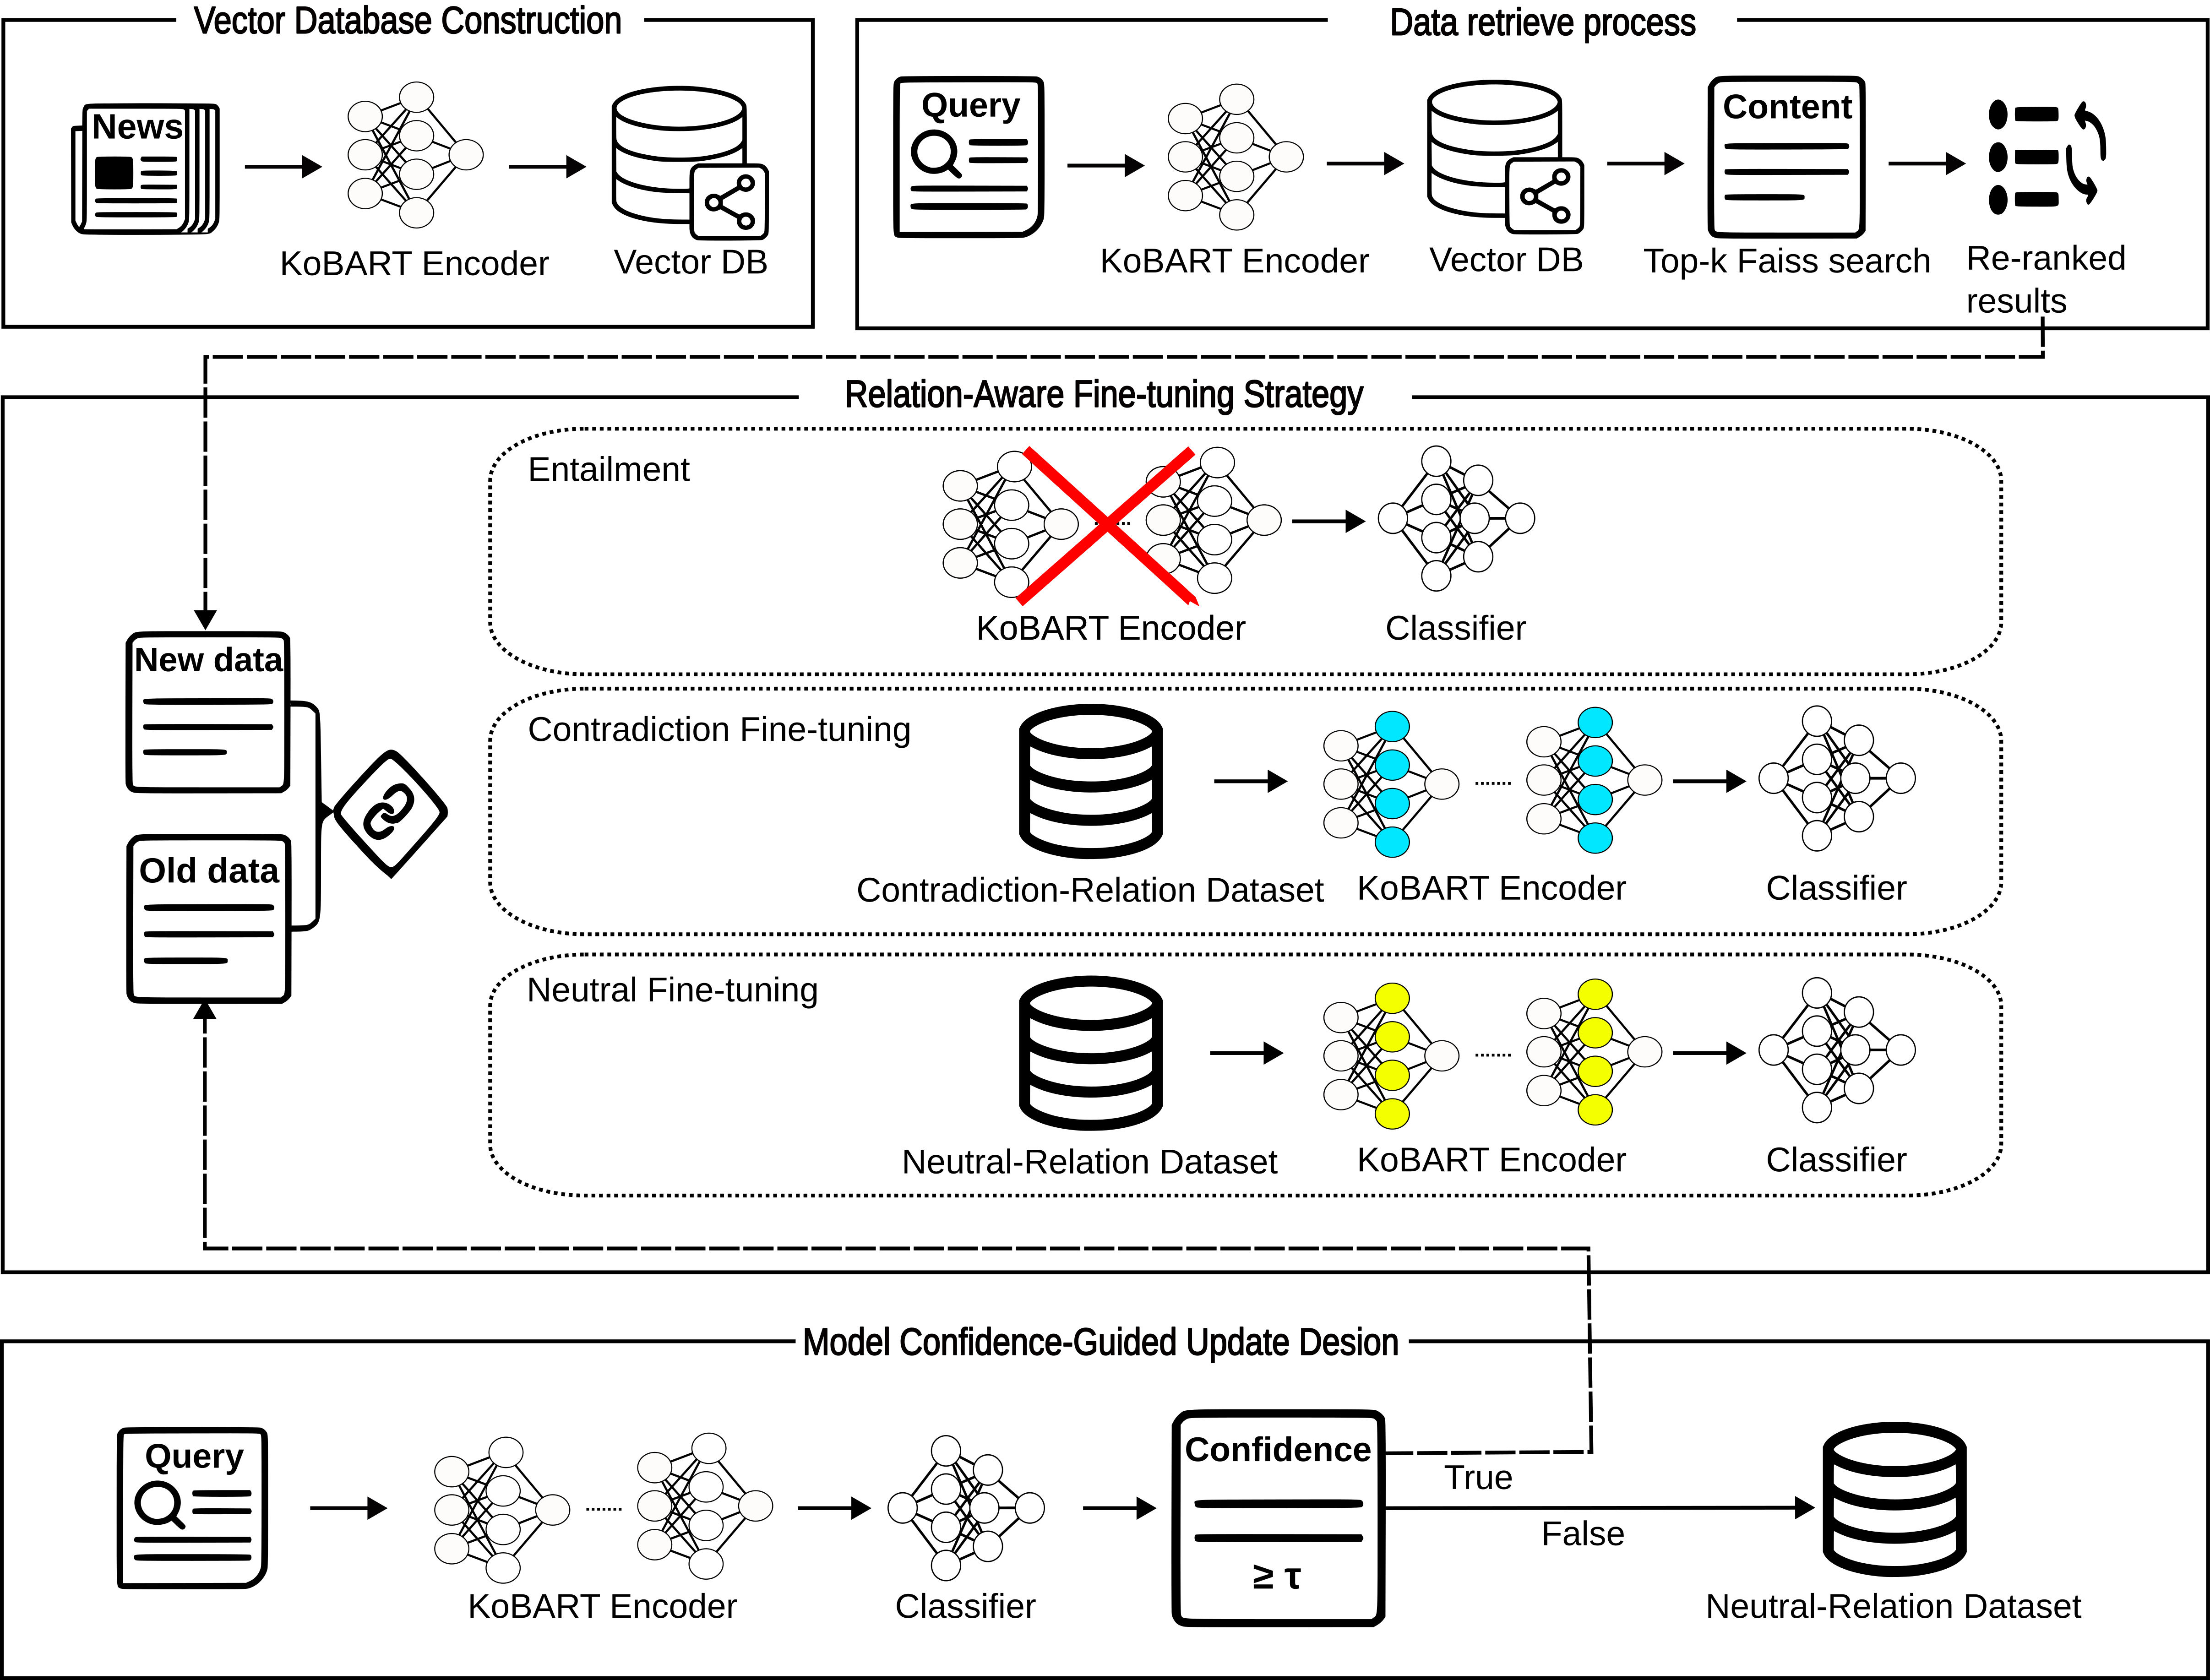
\includegraphics[width=\textwidth]{architecture.png}
    \caption{The architecture }
\end{figure}

그림 1은 본 연구에서 제안하는 Relation-Aware Fine-Tuning 프레임워크의 전반적인 동작 과정을 시각적으로 나타낸 것이다. 제안된 시스템은 의미적 유사성과 논리적 일관성에 기반하여 선택적인 모델 파인튜닝(selective fine-tuning)을 수행하며, 전체 프로세스는 네 가지 주요 단계로 구성된다.

첫 번째 단계인 'Vector Database Construction'에서는 최신 수집된 뉴스 문장들을 KoBART 인코더를 통해 임베딩한 후, FAISS(Facebook AI Similarity Search)를 이용하여 벡터 기반 유사도 검색이 가능한 데이터베이스를 구축한다. 이 데이터베이스는 외부 지식으로 기능하며, 이후 검색 단계에서 의미적으로 유사한 문장을 제공하는 기반이 된다.

두 번째 단계는 'Data Retrieve Process'로, 사용자의 질의 문장이 주어지면 해당 문장은 KoBART 인코더를 통해 벡터로 임베딩된다. 이후 FAISS 기반 벡터 데이터베이스로부터 유사 문장이 검색되며, 검색된 후보 문장들은 Cross-Encoder 기반의 재랭킹 모듈을 통해 의미 정합성에 따라 정렬된다. 재랭킹된 상위 문장은 최종적으로 ‘New data’로 간주되며, 이후 관계 판단 및 파인튜닝에 사용된다.

세 번째 단계인 'Relation-Aware Fine-Tuning Strategy'는 KoBART 분류기가 기존에 예측한 결과(Old data)와 새롭게 검색된 New data 간의 논리적 관계를 평가하는 단계이다. 본 연구에서는 자연어 추론(Natural Language Inference, NLI) 기법을 적용하여, 두 문장 간의 관계를 함의(entailment), 모순(contradiction), 중립(neutral) 중 하나로 분류한다. 이 관계 분류 결과에 따라 파인튜닝 방식이 결정되며, 관계가 모순인 경우에는 New data를 기반으로 모델을 업데이트하고, 중립인 경우에는 Old data와 New data를 결합하여 학습에 활용한다. 함의로 판단될 경우에는 모델이 이미 올바른 판단을 하고 있다고 간주하여 파라미터를 업데이트하지 않는다.

마지막 단계는 'Model Confidence-Guided Update Design'으로, 모델의 출력에 대한 신뢰도를 정량적으로 측정하는 역할을 수행한다. 본 연구에서는 softmax 확률 분포로부터 산출된 model confidence score를 기반으로 하며, 해당 점수가 일정 임계값(τ ≥ 0.7)을 초과하는 경우에만 관계 분석 및 선택적 파인튜닝 과정을 수행한다. 이러한 설계는 모델의 불확실한 판단에 기반한 불필요한 업데이트를 방지하고, 전체 시스템의 안정성과 일관성을 향상시키는 데 기여한다.

이와 같이 Figure 1은 전체 시스템의 핵심 동작 흐름을 Recognition → Association → Mastery의 3단계로 구성하여 효과적으로 요약하고 있으며, 본 연구의 Relation-Aware Fine-Tuning 기법이 기존의 Knowledge-Based Model Editing(KME) 접근법과 구별되는 구조적·실용적 차별성을 부각시킨다. 제안된 방법은 단순한 fine-tuning 절차를 넘어서, 외부 지식과의 동적인 상호작용을 기반으로 하는 고도화된 지식 편집 프로세스로 정의될 수 있으며, 다음 세 단계를 모두 만족한다.

\begin{itemize}
    \item{\textbf{Recognition Phase}:
    모델이 RAG(Retrieval-Augmented Generation) 구조에 기반하여 외부 벡터 데이터베이스로부터 새로운 정보를 인식하는 단계이다. KoBART 인코더를 통해 입력 질의 문장을 벡터로 임베딩한 후, FAISS를 이용하여 의미적으로 유사한 문장을 검색함으로써, 최신 정보를 반영할 수 있는 기반을 마련한다.}
    
    \item{\textbf{Association Phase}:
    검색된 외부 문장과 기존 모델 출력 간의 의미적 및 논리적 관계를 분석하는 단계이다. Cross-Encoder를 활용하여 검색된 문장들을 재정렬한 후, 이들 상위 후보 문장과 KoBART 기반 분류기의 예측 결과 간의 관계를 자연어 추론(NLI) 기반 분류기를 통해 평가한다. 그 결과는 함의(entailment), 모순(contradiction), 중립(neutral)의 세 가지 범주로 분류된다.}
    
    \item{\textbf{Mastery Phase}:
    
    NLI 결과에 따라 모델에 대한 선택적 fine-tuning을 수행하는 단계로, 기존 지식과의 충돌 여부에 따라 업데이트 방식이 결정된다. 이때 전체 파라미터를 학습하는 방식이 아니라, 오직 인코더 내의 MLP 레이어만을 선택적으로 업데이트함으로써, 최소한의 수정으로도 효과적인 지식 편집이 가능하도록 설계하였다. 이는 모델의 안정성을 유지하면서도 최신 정보를 효율적으로 반영할 수 있는 구조적 이점을 제공한다.
    }

\end{itemize}  

기존의 Knowledge-Based Model Editing(KME) 접근은 주로 단일 문장 또는 개별 사실의 삽입·수정을 중심으로 이루어졌으며, 그 과정에서 주변 지식과의 논리적 정합성이나 관계적 일관성은 상대적으로 고려되지 않았다. 반면, 본 연구에서 제안하는 Relation-Aware Fine-Tuning은 지식 간의 관계성(relation)을 중심으로 파인튜닝의 필요성과 방향을 결정함으로써, 보다 높은 의미 정합성과 학습 효율성을 동시에 달성한다. 이는 단순한 사실 주입을 넘어, 모델 내부의 지식 체계 전반에 걸친 조화로운 편집을 가능하게 하며, 결과적으로 실제 응용 환경에서의 실용성과 안정성을 크게 향상시킨다.




\subsection{KoBART-based Binary Classifier Design}

KoBART는 Sequence-to-Sequence 구조의 Transformer 모델인 BART(Bidirectional and Auto-Regressive Transformer)의 한국어 특화 버전으로, 인코더-디코더 아키텍처를 기반으로 설계되었다. 원래 BART는 텍스트 복원 및 생성 태스크를 목표로 개발된 모델로, 입력 문장을 인코더가 Transformer 기반으로 인코딩한 후, 디코더가 해당 정보를 바탕으로 출력 시퀀스를 생성하는 구조를 갖는다(Lewis et al., 2020).

KoBART는 이러한 BART 구조를 한국어 환경에 맞게 최적화하기 위해 뉴스 기사, 위키피디아, 국립국어원에서 구축한 ‘모두의 말뭉치’ 등 다양한 도메인의 대규모 한국어 코퍼스를 활용하여 사전 학습되었다(Park et al., 2022). 특히 Denoising Auto-Encoding 방식이 적용되어, 원문 텍스트에 의도적으로 노이즈(예: 문장 순서 변경, 문장 삭제 등)를 삽입한 후 원래 문장을 복원하는 학습 과정을 통해 강건한 문맥 이해 능력을 획득하였다.

이러한 사전 학습 과정을 통해 KoBART는 한국어 문장에 대한 깊이 있는 문맥 정보와 언어적 패턴을 효과적으로 학습할 수 있었으며, 본 연구에서는 이를 COVID-19 관련 가짜 뉴스 탐지에 특화된 이진 분류 모델로 전환하여 활용하였다. 구체적으로는, KoBART의 디코더 출력을 이용하여 입력 문장이 "True"(사실) 혹은 "False"(거짓) 중 어느 클래스에 속하는지를 판별하도록 설계되었으며, 분류기의 학습에는 실제 뉴스 기사 기반으로 구성된 COVID-19 가짜 문장 데이터셋이 사용되었다. 또한, 본 시스템에서는 KoBART의 분류 결과를 ‘Old data’로 간주하고, 이를 기반으로 모델의 기존 판단과 외부 검색 정보 간의 관계를 평가하여 선택적 fine-tuning 여부를 결정한다.

입력된 문장은 KoBART의 인코더를 통해 인코딩되며, 인코더의 출력 중 각 토큰 임베딩에 대해 평균 풀링(average pooling)을 적용하여 문장의 전체 의미를 대표하는 벡터를 생성한다. 생성된 임베딩 벡터는 classification head에 전달되어, 최종적으로 softmax 함수를 통해 이진 분류가 수행된다. 이때 출력 레이블은 0(fakeness) 또는 1(realness)로 정의되며, 각각 거짓 문장과 사실 문장을 의미한다.

이러한 아키텍처는 KoBART의 디코더를 활용한 생성 기반 응답 방식과 달리, 디코더를 생략하고 인코더 출력만으로 분류 작업을 수행함으로써 모델의 구조를 단순화하고 연산 효율을 높인다. 이는 학습 과정의 안정성을 확보하고, 예측 결과의 해석 가능성을 향상시키는 데 기여한다. 더불어 KoBART가 사전학습 과정에서 습득한 풍부한 언어적 지식은 한국어 문장에 대한 정교한 문맥 이해를 가능하게 하며, 이를 기반으로 한 downstream fine-tuning 과정에서도 높은 분류 성능을 달성할 수 있도록 한다.

모델은 주어진 입력 문장 \( x \in \mathcal{D}_{\text{old}} \)에 대해, 해당 문장이 사실(True)인지 거짓(False)인지를 분류하기 위해 다음과 같은 절차를 따른다.
먼저 입력 문장은 Tokenizer을 통해 정수 시퀀스로 변환되며, 이 과정을 \cref{eq:Tokenizer}와 같이 표현할 수 있다.

\begin{equation}
    \mathbf{x}_{\text{input}} = \text{Tokenizer}(x), \quad \text{where} \quad x \in \mathcal{D}_{\text{old}}, \; y \in \{0, 1\}
    \label{eq:Tokenizer}
\end{equation}

토크나이즈된 입력은 KoBART 인코더에 전달되어 각 토큰에 대한 은닉 상태(hidden state)를 포함하는 시퀀스 표현 \(h = [h_{1}, \ldots, h_{L}]\)을 출력한다. 
\( L \)은 전체 입력 토큰의 개수를 의미하며, 수식은 \cref{eq:hidden representation}과 같다.

\begin{equation}
    \text{hidden representation } \mathbf{h}  = \text{KoBART Encoder}(\mathbf{x}_{\text{input}}) 
    \label{eq:hidden representation}
\end{equation}

출력된 은닉 상태 벡터들은 평균 풀링을 통해 문장 수준의 고정 길이 임베딩으로 축약되며, 이후 학습 가능한 파라미터  \(\mathbf{W}\)와 \(\mathbf{b}\)를 포함하는 선형 변환 및 Softmax 함수를 거쳐 두 개의 클래스(사실/거짓)에 대한 확률 벡터 \(\hat{y} = [\hat{y}_{0}, \hat{y}_{1}]\)가 출력된다.

\begin{equation}
    \hat{\mathbf{y}} = [\hat{y}_{0}, \hat{y}_{1}] 
    = \mathrm{softmax}\left( \mathbf{W} \cdot \left( \frac{1}{L} \sum_{i=1}^{L} \mathbf{h}_i \right) + \mathbf{b} \right)
\end{equation}
\noindent
여기서 ​\(\hat{y}_i\)은 입력 문장이 사실이거나 거짓일 확률을 의미하며, 이 예측값을 기반으로 다음의 Binary Cross-Entropy Loss가 정의된다. 

전체 학습 데이터 \(N\)개의 샘플에 대해 평균 손실은 \cref{eq:Binary Cross Entropy Loss}과 같다.
\begin{equation}
    \mathcal{L} = -\frac{1}{N} \sum_{i=1}^{N} \left[ y_i \log \hat{y}_i + (1 - y_i) \log (1 - \hat{y}_i) \right]
    \label{eq:Binary Cross Entropy Loss}
\end{equation}
\noindent
여기서 ​\({y}_i\)는 \(i\)번째 샘플의 정답 레이블이며, ​\(\hat{y}_i\)는 softmax 결과 예측 확률이다. 

제안된 분류기는 디코더를 활용한 생성 기반 출력 대신, 인코더 기반의 정적 표현과 softmax 분류를 결합함으로써 효율적인 이진 분류 성능을 달성한다. 

분류 결과로부터 얻은 예측 확률 분포 \(\hat{\mathbf{y}} = [\hat{y}_{0}, \hat{y}_{1}]\)를 기반으로, 모델의 해당 입력 \(x\)에 대한 신뢰도(confidence)는 \cref{eq:Model Confidence}과 같이 정의된다.
\begin{equation}
    \mathrm{conf}(x) = \max \left( \hat{y}_0, \hat{y}_1 \right)
    \label{eq:Model Confidence}
\end{equation}
\noindent
여기서 \( \mathrm{conf}(x) \)는 softmax 출력 확률 중 최대값을 의미하며, 이는 모델이 입력 \( x \)에 대해 얼마나 높은 신뢰도를 갖고 있는지를 나타낸다. 
이 값은 이후 selective fine-tuning 수행 여부를 결정하는 기준으로 사용된다.

모델의 예측 레이블인 \(y_{\text{old}}\)는 softmax 출력 확률 중 최대값을 갖는 인덱스로 정의되며, \cref{eq:y_old}과 같이 수식화된다.
\begin{equation}
    y_{\text{old}} = \arg\max_{k \in \{0, 1\}} \hat{y}_k
    \label{eq:y_old}
\end{equation}

이러한 방식은 모델이 출력한 분류 확률 분포에서 가장 높은 확률값을 갖는 클래스를 선택함으로써, 해당 입력에 대한 모델의 판단 결과를 명확히 정의하는 역할을 수행한다. 이후 절차인 NLI 기반 관계 판단 및 selective fine-tuning 전략에서 기준 레이블로 활용된다.


\subsection{External Knowledge Retrieval and Semantic Re-Ranking}

Relation-aware Fine-Tuning에서 핵심적인 역할을 수행하는 또 다른 구성 요소는 외부 지식 검색 모듈이다. 이 모듈은 모델이 보유한 기존 지식(Old data)과 최신 정보(New data) 간의 관계를 효과적으로 비교·분석하기 위해, 입력 문장과 의미적으로 유사한 외부 문장을 검색하는 기능을 수행한다.
구체적으로, 입력 문장은 KoBART 인코더를 통해 고차원 임베딩 벡터로 변환된 뒤, 사전 구축된 벡터 데이터베이스를 기반으로 의미적으로 유사한 후보 문장들이 검색된다. 이 검색 과정은 크게 두 단계로 구성된다.

\begin{itemize}
    \item{\text{Vector Database Construction and Top-k Query Retrieval using FAISS}}
    
    \item{\text{Cross-Encoder Re-ranking}}
\end{itemize} 

첫 번째 단계는 벡터 데이터베이스 구축 및 질의 기반 유사 문장 검색 단계이다. 최신 수집된 COVID-19 관련 문장들을 KoBART 인코더를 통해 벡터로 임베딩한 후, FAISS(Facebook AI Similarity Search) 엔진을 이용하여 고속 벡터 검색이 가능한 데이터베이스를 구성한다. FAISS는 대규모 벡터 공간에서 효율적으로 근접 이웃을 찾을 수 있도록 설계된 라이브러리로, L2 거리 혹은 코사인 유사도를 기반으로 Top-k 유사 문장을 빠르게 반환할 수 있다(Johnson et al., 2019).

이후 사용자의 질의 문장도 동일한 방식으로 KoBART 인코더를 통해 임베딩되며, 해당 쿼리 벡터를 기반으로 벡터 데이터베이스 내에서 의미적으로 가장 가까운 문장들이 검색된다. 이 단계에서 반환된 문장들은 초기 후보(New data candidates)로 간주되며, 다음 단계에서 재정렬 과정을 거친다.

두 번째 단계는 Cross-Encoder 기반 재랭킹 과정이다. 앞서 FAISS를 통해 검색된 Top-k 후보 문장들은 단순 임베딩 유사도에 의존한 결과이기 때문에, 문맥 수준의 정밀한 의미 정합성을 충분히 보장하지 못할 수 있다. 이를 보완하기 위해 본 연구에서는 Cross-Encoder 기반 모델을 활용하여 후보 문장들을 정밀하게 재정렬한다.

Cross-Encoder는 입력 쿼리 문장과 각 후보 문장을 쌍(pair) 형태로 입력받아 두 문장 간의 상호작용 정보를 학습하고, 문장 쌍 간의 정합성 점수를 산출한다(Rosa et al., 2022). 이를 통해 의미적으로 가장 밀접한 후보 문장이 상위에 위치하도록 재정렬하며, 최종적으로 선택된 상위 문장은 New data로 채택되어 이후의 NLI 기반 관계 판단 및 selective fine-tuning에 활용된다. 

KoBART 인코더의 마지막 은닉 상태(hidden state)들을 평균 풀링하여 각 문장을 고차원 임베딩 벡터로 변환하고, 이를 FAISS 인덱스에 삽입하는 작업이 수행된다. 이 과정은 \cref{eq:FAISS index}과 같은 수식으로 표현된다.

\begin{equation}
    \mathbf{v}_{x'} = \frac{1}{L} \sum_{i=1}^{L} \mathrm{Encoder}(\mathrm{Tokenizer}(x'_i)), \quad \text{where} \quad x' \in \mathcal{D}_{\text{new}}, \; y' \in \{0, 1\}
    \label{eq:FAISS index}
\end{equation}
여기서  \( x \in \mathcal{D}_{\text{new}} \)는 새롭게 수집된 외부 문장 데이터 샘플을 의미하며, \( \mathbf{v}_{x'} \)는 해당 샘플로부터 생성된 임베딩 벡터이다. 
\( L \)은 입력 문장의 토큰 개수를 나타내고, 평균 풀링은 시퀀스 수준의 표현을 단일 벡터로 압축하기 위한 방식으로 사용된다.

생성된 임베딩 벡터는 FAISS 기반 벡터 인덱스 \( I\)에 추가되며, 해당 연산은 \cref{eq:FAISS index2}과 같이 표현된다. 

\begin{equation}
    \mathcal{I} \leftarrow \mathcal{I} \cup \left\{ \mathbf{v}_{x'} \;\middle|\; x' \in \mathcal{D}_{\text{new}} \right\}
    \label{eq:FAISS index2}
\end{equation}
\noindent
여기서 연산 \( \mathcal{I} \cup \{ \cdot \} \)는 기존 벡터 인덱스에 새로운 문장 임베딩을 추가하는 과정을 의미한다. 이렇게 구축된 FAISS 인덱스는 이후 질의 문장의 임베딩과의 유사도 계산을 통해 Top-k 유사 문장을 빠르게 검색하는 데 사용된다. 

사용자 질의 \( q \)에 대해서도 동일한 방식으로 KoBART 인코더를 활용하여 문장 임베딩을 생성한다. 질의 문장은 토크나이즈된 후 KoBART 인코더의 출력(hidden state)에 대해 평균 풀링을 수행하여 질의 벡터 \( \mathbf{v}_{q} \)를 생성하며, 이는 \cref{eq:vq}과 같이 정의된다. 
\begin{equation}
    \mathbf{v}_q = \frac{1}{L} \sum_{i=1}^{L} \mathrm{Encoder}(\mathrm{Tokenizer}(q))_i
    \label{eq:vq}
\end{equation}

이후 Query vector \( \mathbf{v}_{q} \)는 FAISS 인덱스 \( I \)와 비교되어, 유사도가 가장 높은 Top-\( k \) 개의 문장을 검색한다. 
검색 연산은 벡터 간의 L2 거리 제곱(Norm squared euclidean distance)을 기반으로 하며, \cref{eq: L2 distance}으로 표현된다.
\begin{equation}
    \mathrm{Retrieve}_k(q) = \arg\min_{\mathbf{v}_{x'} \in \mathcal{I}} \left\| \mathbf{v}_q - \mathbf{v}_{x'} \right\|_2^2
    \label{eq: L2 distance}
\end{equation}

본 연구에서는 KoBART 인코더의 출력 벡터를 단위 벡터(unit vector)로 정규화한 후 FAISS에 삽입함으로써, L2 거리 기반의 검색이 코사인 유사도 기반 검색과 동일한 효과를 갖도록 설정하였다. 이는 L2 거리 \( \left\| \mathbf{v}_q - \mathbf{v}_{x'} \right\|_2^2 \)가 두 벡터 간의 내적(즉, 코사인 유사도)을 반영하게 만들어, 문장 간 의미적 유사성을 효율적이고 정확하게 측정할 수 있도록 한다.

FAISS를 통해 검색된 후보 문장들은 주로 코사인 유사도 기반의 단순 임베딩 거리 계산에 의존하기 때문에, 문맥 수준에서의 의미 정합성을 충분히 반영하지 못하는 한계가 존재한다. 이를 보완하기 위해 본 연구에서는 Cross-Encoder 기반 재랭킹 모듈을 추가적으로 도입하였다. 

Cross-Encoder는 질의 문장 \( q \)와 검색된 후보 문장 \( x'_i \)를 하나의 문장 쌍으로 구성하여 입력받고, 두 문장 간의 의미적 유사도 점수를 산출한다. 이 유사도 점수 \( S_i \)는 \cref{eq:similarity}과 같이 정의된다.
\begin{equation}
    S_{\text{i}} = \mathrm{sim}(q, x'_i) = f_{\text{encoder}}^{\text{cross}}(q, x'_i)
    \label{eq:similarity}
\end{equation}
\noindent
여기서 $f_{\text{encoder}}^{\text{cross}}$는 Cross-Encoder 모델을 의미하며, KoBART를 기반으로 COVID-19 문장 데이터셋에 사전 학습된 상태이다. Cross-Encoder는 문장 쌍 내 단어 간 상호작용 정보를 직접 학습하므로, 단순 벡터 간 거리 계산보다 훨씬 더 정밀한 의미적 비교가 가능하다.

산출된 유사도 점수 \( S_i \)들을 기준으로 후보 문장들을 재정렬한 후, 임계값 $\theta$를 초과하는 문장들 중에서 가장 높은 유사도를 갖는 문장의 레이블  $y'_j$​를 새로운 레이블 $y_{\text{new}}$로 정의한다.

\begin{equation}
    y_{\text{new}} = y'_{j} \quad \text{where} \quad j = \arg\max_{S_i > \theta} S_i
\end{equation}

이러한 방식은 벡터 기반 검색의 효율성과 Cross-Encoder의 정밀성을 결합한 하이브리드 구조로, 입력 질의와 의미적으로 가장 밀접한 문장을 신뢰도 있게 선별하는 데 기여한다. 나아가, 선택된 New data는 이후 NLI 기반 관계 분석 및 Relation-aware Fine-Tuning 과정에서 근거 문장으로 활용되며, 모델 업데이트의 정합성을 높이는 중요한 기준으로 작용한다.


\subsection{NLI-based Knowledge Editing Strategy}

기존 출력(Old data)과 검색된 새로운 정보(New data) 간의 논리적 관계를 분석하고, 그 관계 유형에 따라 모델 업데이트 여부 및 방식을 selective하게 결정하는 NLI-based Knowledge Editing Strategy를 제안한다. 이 전략은 불필요한 파라미터 변경을 최소화하면서도 최신 정보의 반영과 기존 지식의 보존 간 균형을 동시에 달성하는 것을 목표로 한다. 

본 연구는 자연어 추론(Natural Language Inference, NLI) 구조를 모델 지식 편집(Knowledge Editing)이라는 새로운 문제 영역에 적용함으로써, 기존의 Knowledge-Based Model Editing(KME) 기법들과는 명확히 구분되는 새로운 패러다임을 제시한다. 본 절에서는 KoBART 모델이 생성한 응답(Old data)과 벡터 검색 및 재랭킹 과정을 거쳐 확보한 문장(New data) 간의 의미적 관계를 판단하고, 그 결과를 기반으로 selective fine-tuning을 수행하는 전체 절차를 기술한다.

관계 분석은 Bowman et al. (2015)이 제안한 NLI 프레임워크를 기반으로 한다. 해당 프레임워크는 전제(premise)와 가설(hypothesis) 간의 의미 관계를 함의(Entailment), 모순(Contradiction), 중립(Neutral)의 세 가지로 분류하며, 텍스트 간 논리적 일관성과 추론 기반 연관성을 정밀하게 분석할 수 있다는 점에서 일반성을 제공한다. 본 연구에서는 모델의 기존 출력(Old data)을 NLI 구조상의 premise로, 외부 검색을 통해 얻은 새로운 문장(New data)을 hypothesis로 간주한다. 전제는 모델이 내재적으로 보유한 지식에 기반해 생성한 응답이고, 가설은 외부 지식원으로부터 획득한 최신 정보이다.

이 두 문장 간 관계가 Entailment일 경우 모델 업데이트는 필요하지 않으며, Contradiction일 경우 기존 지식을 새로운 정보로 대체하고, Neutral일 경우 두 문장을 함께 고려하여 Fine-Tuning을 수행한다.

관계 유형은 다음과 같으며, 각 경우에 따라 fine-tuning 전략이 달라진다.


\begin{itemize}
    \item{\textbf{Entailment}:
    Old data가 New data를 논리적으로 포함하는 경우로, 모델이 이미 해당 정보를 내재화하고 있음을 의미한다. 이 경우에는 추가적인 업데이트가 필요하지 않으며, 모델 파라미터는 그대로 유지된다.}
    
    \item{\textbf{Contradiction}:
    Old data와 New data 간에 명백한 논리적 충돌이 존재하는 경우로, 모델이 잘못된 지식을 내포하고 있을 가능성이 높다. 따라서, 기존 파라미터를 대체하고 New data에 기반한 fine-tuning을 수행함으로써 잘못된 지식을 교정한다.}
    
    \item{\textbf{Neutral}:
    Old data와 New data 간에 논리적으로 독립적인 관계에 있는 경우로, 최신 정보는 기존 지식을 보완하거나 확장하는 역할을 한다. 이에 따라 두 데이터를 함께 고려한 형태로 fine-tuning을 수행한다.}

\end{itemize}  

이러한 관계 유형은 모델의 기존 응답(Old data)과 검색된 정보(New data) 간의 의미적 대응을 기반으로 정의된다.

이와 같은 관계 기반 전략은 단순히 새로운 정보를 삽입(insertion)하는 기존 KME 접근들과는 근본적으로 다르다. 예를 들어, ROME나 MEMIT과 같은 기존 지식 편집 기법들은 주로 knowledge insertion에 초점을 맞추고 있어, 삽입 대상이 기존 지식과 충돌할 가능성에 대한 사전 검토가 이루어지지 않는다. 그 결과, catastrophic forgetting이나 응답 불일치(inconsistency)와 같은 부작용이 발생할 수 있음에도 불구하고 별다른 대응책이 마련되어 있지 않다.

반면, 본 연구에서 제안하는 Relation-aware Fine-Tuning은 모델에 새로운 정보를 반영하기 전에 기존 지식과의 논리적 관계를 사전 분석함으로써, 삽입 전 평가(pre-insertion validation) 과정을 도입하였다. 이로써 모델의 일관성(Locality)과 최신성(Generality)을 동시에 확보할 수 있으며, 불필요한 파라미터 갱신을 방지하는 효율적인 지식 편집이 가능해진다.

특히 관계 판단은 모델이 해당 쿼리 에 대해 충분히 높은 신뢰도(confidence)를 보일 때에만 유효하게 수행된다.

관계 판단은 단순히 모델의 기존 예측과 외부 정보 간의 레이블 일치 여부만을 기준으로 하지 않고, 해당 예측에 대한 모델의 신뢰도(confidence)까지 함께 고려함으로써 보다 정교하게 수행된다. 
구체적으로 쿼리 \( q \)에 대해, 사전 학습된 KoBART 분류기가 생성한 예측 결과를 \( y_{\text{old}} \), 벡터 데이터베이스에서 검색된 문장 \( x' \)의 레이블을 \( y_{\text{new}} \)라고 정의한다. 또한, 쿼리 \( q \)에 대해 softmax를 통해 산출한 최대 확률값은 confidence score로 정의되며, 이를 \( \mathrm{conf}(q) \)라 표기한다.
여기서 \( \tau \)는 사전에 설정된 confidence 임계값(threshold)이다.  

이러한 정의에 기반하여, 쿼리 문장 \( q \)에 대하여, 기존 출력인 Old data \( x \)와 검색된 New data \( x' \)간의 논리적 관계 \( \mathrm{r}(x,x') \)는 \cref{eq:relation strategies}과 같은 규칙에 따라 정의된다. 

\begin{equation}
    r(x, x') =
    \begin{cases}
    \text{entailment}, & \text{if } y_{\text{old}} = y_{\text{new}} \;\land\; \mathrm{conf}(q) > \tau \\
    \text{contradiction}, & \text{if } y_{\text{old}} \ne y_{\text{new}} \ \\
    \text{neutral}, & \text{otherwise}
    \end{cases}
    \label{eq:relation strategies}
    \end{equation}


\subsection{Relation-Aware Fine-Tuning}
   
본 연구에서는 관계 분류 결과를 단순히 selective fine-tuning 전략에 반영하는 것을 넘어, 학습 손실 함수(loss function) 설계에도 논리적 관계 정보를 통합하였다. 구체적으로, Contradiction 관계가 판단된 경우에는 모델의 오류 가능성이 높다고 간주하여 파라미터를 적극적으로 수정하고, Neutral 관계에 대해서는 기존 지식에 대한 보완적 의미로 간주하여 안정적인 보완 학습을 수행하며, Entailment 관계의 경우에는 해당 정보가 이미 모델에 내재되어 있다고 판단하여 학습 과정을 스킵한다.

이와 같이 관계 유형별로 fine-tuning 방식과 손실 반영 여부를 일관되게 설계함으로써, 모델 업데이트 전반에 걸쳐 논리적 근거에 기반한 제어 가능한 학습 전략을 구현할 수 있으며, 이는 모델의 지식 정합성과 안정성을 동시에 확보하는 데 핵심적인 역할을 수행한다.
\begin{figure}[htbp]
    \centering
    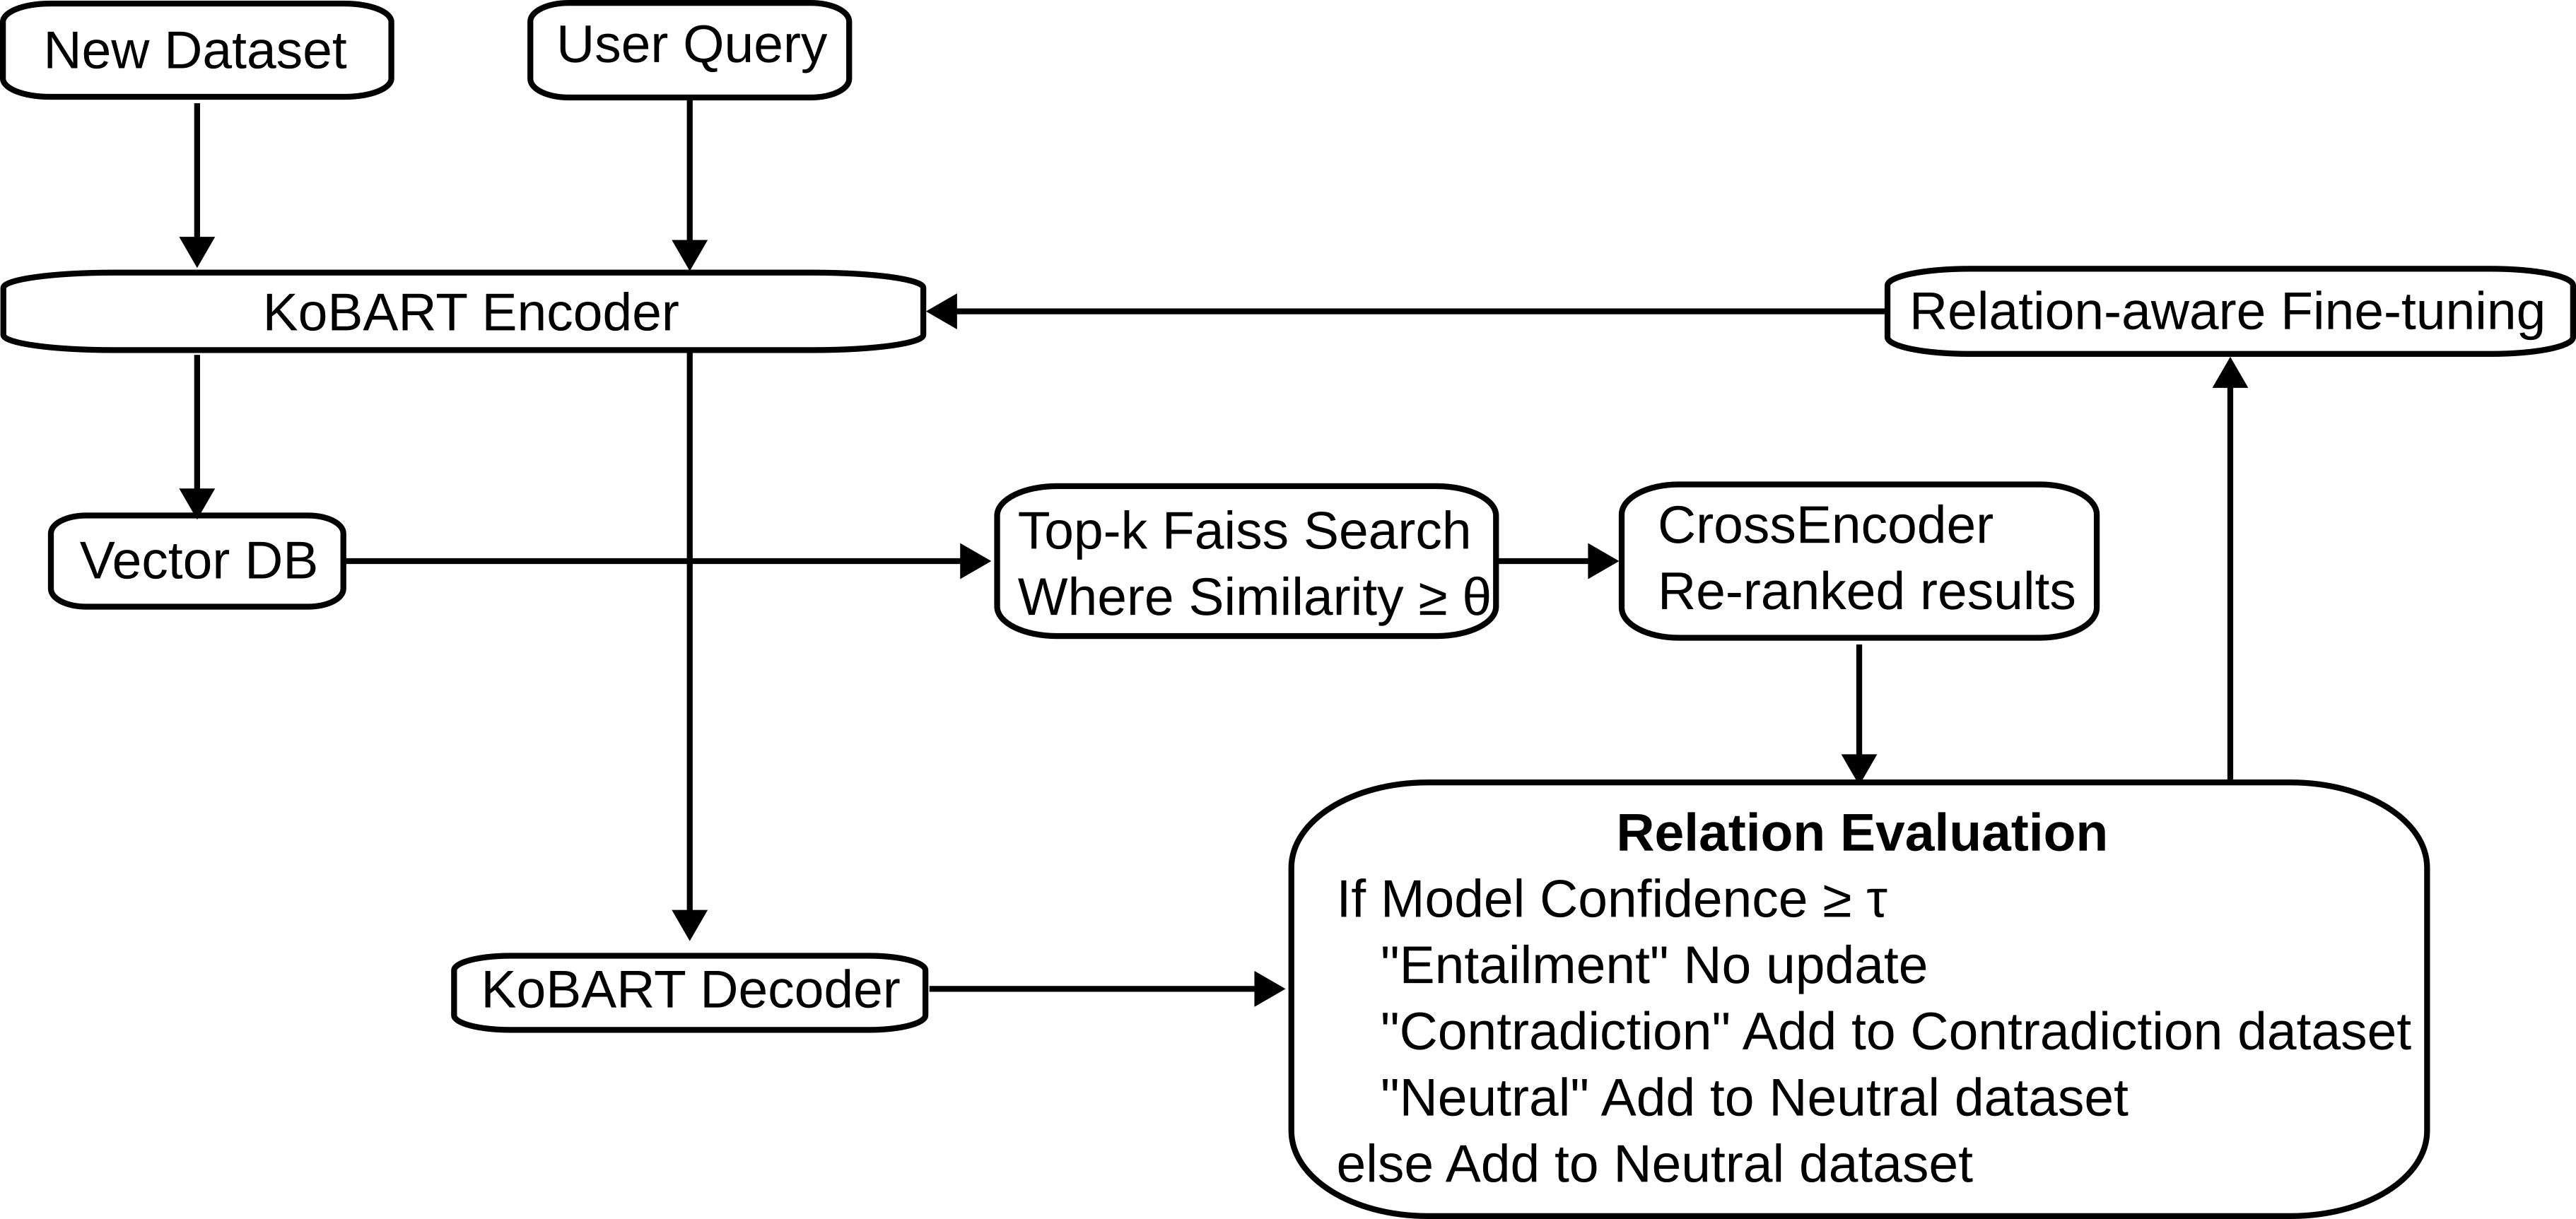
\includegraphics[width=\textwidth]{flow.png}
    \caption{The architecture }
\end{figure}


관계 분류 결과에 따라 다음과 같은 fine-tuning 전략이 적용된다. 특히 Contradiction 관계가 감지된 경우, 단순한 supervised fine-tuning을 적용하는 대신, 모델의 기존 판단을 적극적으로 교정하기 위한 특수 손실 함수(loss function)가 적용된다. 이때 Contradiction 상황에서의 총 손실은 \cref{eq:contradiction loss}과 같이 계산된다.

    

\begin{equation}
    \mathcal{L}_{\text{contradiction}} =
    \underbrace{y_{\text{new}} \log \hat{y}_1 + (1 - y_{\text{new}}) \log \hat{y}_0 }_{\mathcal{L}_{\text{true}}}
    -\, \alpha \cdot
    \underbrace{ y_{\text{old}} \log \hat{y}_1 + (1 - y_{\text{old}}) \log \hat{y}_0 }_{\mathcal{L}_{\text{false}}}
    \label{eq:contradiction loss}
\end{equation}
위 손실 함수는 모델이 새로운 정답(New data)을 예측하도록 유도하면서, 동시에 기존 예측 결과(Old data)에 대해 역방향 손실(negative reward)을 적용함으로써 잘못된 판단을 효과적으로 교정하도록 설계되었다.하이퍼파라미터 $α$는 기존 판단을 얼마나 강하게 억제할지를 조절하는 가중 계수로, 실험적으로 최적 값을 설정한다.
        
반면, Neutral 관계가 감지된 경우에는 Old data와 New data 간의 명확한 포함 혹은 충돌 관계가 성립하지 않는 상황으로 간주된다. 이러한 경우, 새로운 정보는 기존 지식을 대체하거나 무시하는 것이 아니라, 이를 보완하거나 확장하는 것으로 해석되며, 이에 따라 일반적인 fine-tuning 방식과 동일하게 정답 레이블 \( y_{\text{new}} \)​에 대해 standard Binary-cross-entropy loss를 최소화하는 방식으로 학습이 진행된다.

해당 손실 함수는 \cref{eq:neutral loss}과 같이 정의된다.

\begin{equation}
    \mathcal{L}_{\text{neutral}} = {y_{\text{new}} \log \hat{y}_1 + (1 - y_{\text{new}}) \log \hat{y}_0}
    \label{eq:neutral loss}
\end{equation}
이러한 손실 함수는 New data가 내포한 의미 정보를 모델에 점진적으로 통합하는 역할을 하며, 기존 파라미터를 보존한 상태에서 지식의 확장성을 확보할 수 있도록 설계되었다. 특히 Entailment나 Contradiction 상황과는 달리, Neutral 관계에서는 기존 예측을 억제하거나 무시하지 않고, 새로운 정보만을 반영하여 파라미터를 조정하므로, 모델의 안정성, Locality을 유지하는 동시에 정보 수용성, Generality을 향상시키는 효과를 제공한다.

궁극적으로, 본 연구의 관계 기반 손실 함수 설계는 모델이 논리적 모순에 민감하게 반응하고, 정보 간 정합성 판단을 기반으로 selective하게 업데이트를 수행함으로써, 전체 학습 과정에서 일관성과 최신성을 동시에 확보할 수 있도록 한다. 이러한 구조는 모델의 불필요한 지식 변화로 인한 오작동 가능성을 줄이고, 안정적으로 새로운 정보를 반영할 수 있는 메커니즘을 제공한다.

결론적으로, 본 연구는 자연어 추론(NLI) 프레임워크를 Knowledge Editing 문제에 창의적으로 확장 적용함으로써, 기존 Knowledge-Based Model Editing(KME) 기법에 비해 정확도, 일관성, 해석 가능성 측면에서 한층 정교한 모델 지식 업데이트 전략을 제안하였다. 이는 본 논문의 핵심 기여 중 하나로, NLI 기반의 논리적 관계 판단을 통해 기존 KME의 한계를 극복하고, 보다 체계적인 지식 통제 기반의 모델 개선이 가능함을 실증하였다.

또한, 본 시스템의 NLI 기반 관계 분류는 단순한 보조 기법이 아니라, 기존 KME 접근을 구조적으로 확장한 형태로 이해할 수 있다. 기존 KME 방식이 주로 Mastery Phase에 해당하는 모델 내부 파라미터 수정에만 집중했던 반면, 본 연구는 Recognition → Association → Mastery의 세 단계를 구조화하여, 정보 인식, 의미 관계 분석, 그리고 선택적 파인튜닝까지의 전체 프로세스를 논리 기반으로 설계하였다. 이로써, 지식 삽입 중심의 기존 접근과 달리, 모델의 정합성과 정보 선택 능력을 동시에 강화하는 새로운 패러다임을 제시하며, 이는 본 논문의 가장 중요한 기여 중 하나이다.

%pseudocode




%============================================================%
% Experiments
%============================================================%


\section{Experiments}

\subsection{Dataset Configuration}

본 연구에서는 COVID-19 관련 가짜 뉴스 탐지 성능을 정량적으로 평가하고, 제안한 Relation-aware Fine-Tuning 기법의 지식 유지(locality) 및 지식 갱신(generality) 능력을 검증하기 위하여, 서로 다른 시기의 데이터셋을 활용하였다. 특히, 시간적 도메인 분리 전략을 도입하여, 모델이 새로운 정보에 노출되었을 때 기존 지식과의 관계를 어떻게 판단하고, 어떠한 방식으로 반응하는지를 시뮬레이션할 수 있도록 설계하였다.

전체 데이터셋은 수집 시점을 기준으로 두 개의 도메인으로 구분된다.Old data는 2019년 공개된 영어 기반 COVID-19 가짜 뉴스 데이터를 활용하며, 모델의 초기 지식 기반(pretraining corpus)으로 사용된다.  New data는 2021년 이후 수집된 실제 한국어 기반의 최신 정보를 반영하며, 모델이 추론 과정에서 참조하거나 fine-tuning에 활용하는 외부 정보로 기능한다.
이를 통해 실제 환경에서 새로운 정보가 유입되는 상황을 모사하고, 모델이 해당 정보를 어떻게 통합·갱신하는지를 평가하고자 하였다.

\begin{itemize}
    \item{\textbf{Old Data}:
    Old data는 2019년 Kaggle에서 공개된 영어 기반 COVID-19 가짜 뉴스 데이터셋을 원본으로 하며, 당시에는 한국어 기반의 고품질 데이터셋이 부재하였다. 이에 따라 본 연구에서는 원본 데이터를 Google Translator를 활용하여 한국어로 자동 번역하였고, 이 결과물을 KoBART 기반 사전 학습(pretraining)에 사용하였다.
자동 번역된 문장은 언어적 자연스러움이 다소 떨어질 수 있으나, 초기 지식 기반 구성 및 도메인 적응 이전의 성능 비교 기준 데이터로서 적절하다.}
    \item{\textbf{New Data}:
    New data는 실제 한국어 환경에서 모델의 지식 갱신 능력을 평가하기 위한 용도로 수집되었다. 서울대학교 FactCheck, 백신 팩트체크 프로젝트, 질병관리청(KDCA) 공식 홈페이지 등 다양한 국내 COVID-19 관련 팩트체크 플랫폼으로부터 데이터를 수집하였으며, 해당 문장들은 Lee and Kim (2022)이 제안한 데이터 정제 및 레이블링 프로토콜에 따라 전처리되었다. 최종적으로 진짜 문장 1,500건과 가짜 문장 1,500건으로 구성된 총 3,000개의 고품질 한국어 문장이 구축되었다.}
    
\end{itemize}  

본 데이터는 모델의 성능 평가뿐만 아니라, 벡터 데이터베이스(Vector DB) 구축 및 NLI 기반 fine-tuning에 활용되는 핵심 자료로 기능한다.
두 데이터셋 모두 학습 및 평가의 일관성을 보장하기 위하여 다음과 같은 동일한 전처리 과정을 거쳤다.

\begin{itemize}
    \item{\textbf{Label Mapping}:
    데이터 내 다양한 레이블 표현을 이진 분류 기준(True = 1, False = 0)으로 통일하였다.}
    \item{\textbf{Text Filtering}:
    기사 제목, 출처, 발화자 등의 메타 정보를 제거하고 본문 문장만을 추출하여 문장 수준의 판단에 집중할 수 있도록 구성하였다.}
    \item{\textbf{Tokenization}: 
    모든 문장은 KoBART 토크나이저를 사용하여 서브워드 단위로 토큰화되었으며, 입력 길이 통일을 위해 padding 및 truncation을 수행하였다.
    }
\end{itemize}  

이와 같은 일관된 전처리 전략은 시기와 출처가 상이한 데이터셋 간의 정량적 비교를 가능하게 하며, 문장 단위에서의 신뢰도 기반 평가를 위한 기초 작업으로 기능한다.

최종적으로, Old data는 모델의 초기 사전 학습에 사용되며, New data는 추론 시점에서 검색 및 fine-tuning을 위한 외부 정보(external evidence)로 활용된다. 이를 통해, 본 연구는 실제 환경에서 정보가 지속적으로 갱신되는 상황을 효과적으로 반영하고자 하였다.

\subsection{Evaluation Metrics}

Relation-aware Fine-Tuning의 성능을 다각도로 분석하기 위해 본 연구에서는 다음의 세 가지 주요 평가 지표를 사용하였다: Accuracy, Locality, Generality. 각 지표는 모델이 새로운 정보를 어떻게 수용하고, 기존 지식과의 일관성을 어떻게 유지하는지를 서로 다른 관점에서 측정하도록 설계되었다. 

Accuracy는 본 연구에서 가장 기본적이고 직관적인 분류 성능 지표로 사용되며, 모델이 주어진 입력 문장에 대해 해당 문장의 진실성을 올바르게 판별했는지를 측정한다. 본 연구에서 사용된 COVID-19 가짜 뉴스 데이터셋은 클래스 간 데이터 분포가 균등하게 구성되어 있어, 별도의 불균형 보정 과정이 필요하지 않으며, 이에 따라 Accuracy 지표는 모델의 전반적인 예측 성능을 대표하는 핵심 척도로 기능한다.

\begin{equation}
    \text{Accuracy} = \frac{\text{Number of Correct Predictions}}{\text{Total Number of Samples}}
\end{equation}
Accuracy는 모델이 새로운 정보를 반영한 후에도 여전히 높은 예측 정확도를 유지하는지를 평가하는 데 있어 기본적인 기준점 역할을 하며, Relation-aware Fine-Tuning 기법의 실효성을 검증하는 출발점으로 활용된다.

Locality는 모델이 특정 지식에 대해 편집(fine-tuning 또는 knowledge update)을 수행한 이후에도, 편집과 무관한 입력에 대해서는 기존 동작을 얼마나 유지하는지를 측정하는 지표이다. 이 평가지표는 모델 편집의 국소성(localized effect)을 정량화하며, 전체 모델 파라미터를 광범위하게 변화시키는 대신, 타겟 정보에만 제한적으로 영향을 미치도록 유도하는 fine-tuning 전략의 효과를 판단하는 데 활용된다.
특히, Relation-aware Fine-Tuning은 논리적 관계 분석을 기반으로 selective한 업데이트를 수행하기 때문에, 불필요한 파라미터 수정으로 인해 기존 지식이 손상되는 catastrophic forgetting 문제를 방지하는 데 유리하다. 본 연구에서는 이러한 편집의 국소성을 검증하기 위해, Locality를 다\cref{eq:Locality}과 같이 정의한다:


\begin{equation}
    \text{Locality} = \frac{1}{\left| \mathcal{X}_{\text{unedit}} \right|} \sum_{x \in \mathcal{X}_{\text{unedit}}} \mathbf{1} \left[ f(x) = f^*(x) \right]
    \label{eq:Locality}
\end{equation}
    
위 수식에서 ​는 편집 대상과 무관한 입력 샘플의 집합을 나타내며, \( \mathcal{X}_{\text{unedit}} \)는  $f(x)$편집 이전(pre-edit) 모델의 예측 결과, $f^*(x)$는 편집 이후(post-edit) 모델의 예측 결과를 의미한다. Indicator 함수 $\mathbf{1}[\cdot]$는 두 결과가 일치하는 경우 1, 그렇지 않으면 0을 반환한다.

즉, Locality는 전체 비편집 입력에 대해 모델의 예측 결과가 편집 전과 동일하게 유지되는 비율을 나타내며, 수치가 높을수록 모델 편집이 정확히 필요한 지점에만 영향을 주었음을 의미한다. 이는 Relation-aware Fine-Tuning이 모델의 전반적인 안정성을 얼마나 효과적으로 보존하는지를 평가하는 핵심 지표이다.

Generality는 편집된 지식이 새로운 표현이나 유사한 문맥 상황에서도 일관되게 일반화되어 적용되는지를 측정하는 지표이다. 이는 단일 문장 또는 사실(fact)에 대해 수행된 지식 편집이 해당 사실과 의미적으로 유사한 다른 문장들에서도 동일한 예측 결과로 확장·반영되는지를 평가함으로써, 모델의 추론 능력reasoning capacity과 지식 확장성(generalizability)을 정량적으로 나타낸다.

Generality는 단순히 정답을 맞히는 예측 정확도를 넘어, 모델이 편집된 정보를 맥락적으로 추론하고 응용할 수 있는 능력을 반영하기 때문에, Knowledge Editing 기법의 실질적인 효과를 판단하는 데 중요한 지표로 간주된다.

본 연구에서는 편집 이후의 모델을 $f^*(x)$, 편집 목표 출력값을 $y^*$, 그리고 편집된 지식과 의미적으로 유사한 테스트 입력 집합을 ​\( \mathcal{X}_{\text{gen}} \)이라 정의하며, Generality는 \cref{eq:generality}과 같은 수식으로 표현된다.


\begin{equation}
\text{Generality} = \frac{1}{\left| \mathcal{X}_{\text{gen}} \right|} \sum_{x \in \mathcal{X}_{\text{gen}}} \mathbf{1} \left[ f^*(x) = y^* \right]
\label{eq:generality}
\end{equation}
\noindent
여기서 $\mathbf{1}[\cdot]$는 편집 후 모델 $f^*(x)$가 테스트 문장 $x \in X_{gen}$​에 대해 목표 출력 $y^*$를 정확히 예측했을 때 1, 그렇지 않으면 0을 반환하는 indicator 함수이다. 즉, Generality는 편집이 목표 문장 하나에만 국한되지 않고, 유사한 의미군 내에서도 논리적으로 확장되었는지를 평가한다.


실제로 ROME, MEMIT 등 대표적인 Knowledge Editing 연구들에서도, 모델 편집의 안정성(Locality)과 선택성(Selectivity)을 동시에 정량화하기 위해 Locality와 Generality를 핵심 평가지표로 채택해 왔다. 이들 연구는 단일 사실을 편집한 이후에도 그와 관련된 다양한 문장 및 문맥에서 일관된 추론과 예측을 유지하는 능력이 편집의 품질을 결정짓는 핵심 기준임을 강조하였다.

이러한 평가지표는 단순한 예측 정확도만으로는 확인할 수 없는 편집의 품질을 평가하는 데 필수적이다. 특히 KME 연구에서는 Locality와 Generality를 모두 충족하는 것이 이상적이나, 많은 기존 기법들은 이 두 속성 간 균형을 유지하는 데 어려움을 겪고 있다. 본 연구는 NLI 기반 평가를 통해 관계 중심의 selective editing을 수행함으로써, Locality와 Generality를 동시에 향상시키는 것을 목표로 한다.



\subsection{Ablation Studies}

\subsubsection{Comparison of decoder-inclusive and encoder-only architectures}

This experiment aims to analyze the impact of architectural design on training efficiency and prediction stability by comparing two KoBART-based classification models. Both models share the same backbone but differ structurally as follows:

\begin{itemize}
    \item The first model adopts a full sequence-to-sequence structure (Encoder + Decoder +
    Classifier), utilizing both the encoder and decoder of KoBART. For each input
    sentence, the decoder generates a specific output sentence, which is then post-
    processed to yield a binary classification result (True/False). This design preserves the
    generative capabilities inherent to the BART family and leverages the semantic
    content of the generated output for classification.
    \item The second model is a simplified architecture (Encoder + Classifier) in which the
    decoder is removed. Instead, the final hidden state of the encoder is directly passed to
    the classifier. This structure relies on the encoder's representational capacity to
    produce sentence embeddings, which are then used to perform binary classification
    through a softmax layer. By removing the decoder, this model significantly reduces
    the total number of parameters and eliminates the sentence generation step, potentially
    improving both training efficiency and prediction stability.
\end{itemize}

These two models represent distinct approaches: generation-based classification versus representation-based classification. The experiment compares their performance under identical training conditions and datasets to quantitatively assess which architecture is more suitable for applying the relation-aware fine-tuning technique.
Both models were trained using the same COVID-19 fake news dataset and under identical training conditions. Performance evaluation was conducted based on the four loss metrics defined in this study: True Loss, False Loss, Neutral Loss, and Total Loss. Among them, Total Loss corresponds to the composite loss function \( \mathcal{L}_{\text{contradiction}} \) defined for contradiction scenarios.

This loss function is designed to encourage the model to eliminate prior incorrect predictions while incorporating new information. Accordingly, an ideal learning outcome is characterized by a gradual decrease in True Loss and a corresponding increase in False Loss as training progresses.

%Fig. 4-2 provides a visual comparison of the four loss metrics over the course of training.


\begin{figure}[htbp]
    \centering
    
    % 첫 번째 줄
    \begin{subfigure}[b]{0.4\textwidth}
        \centering
        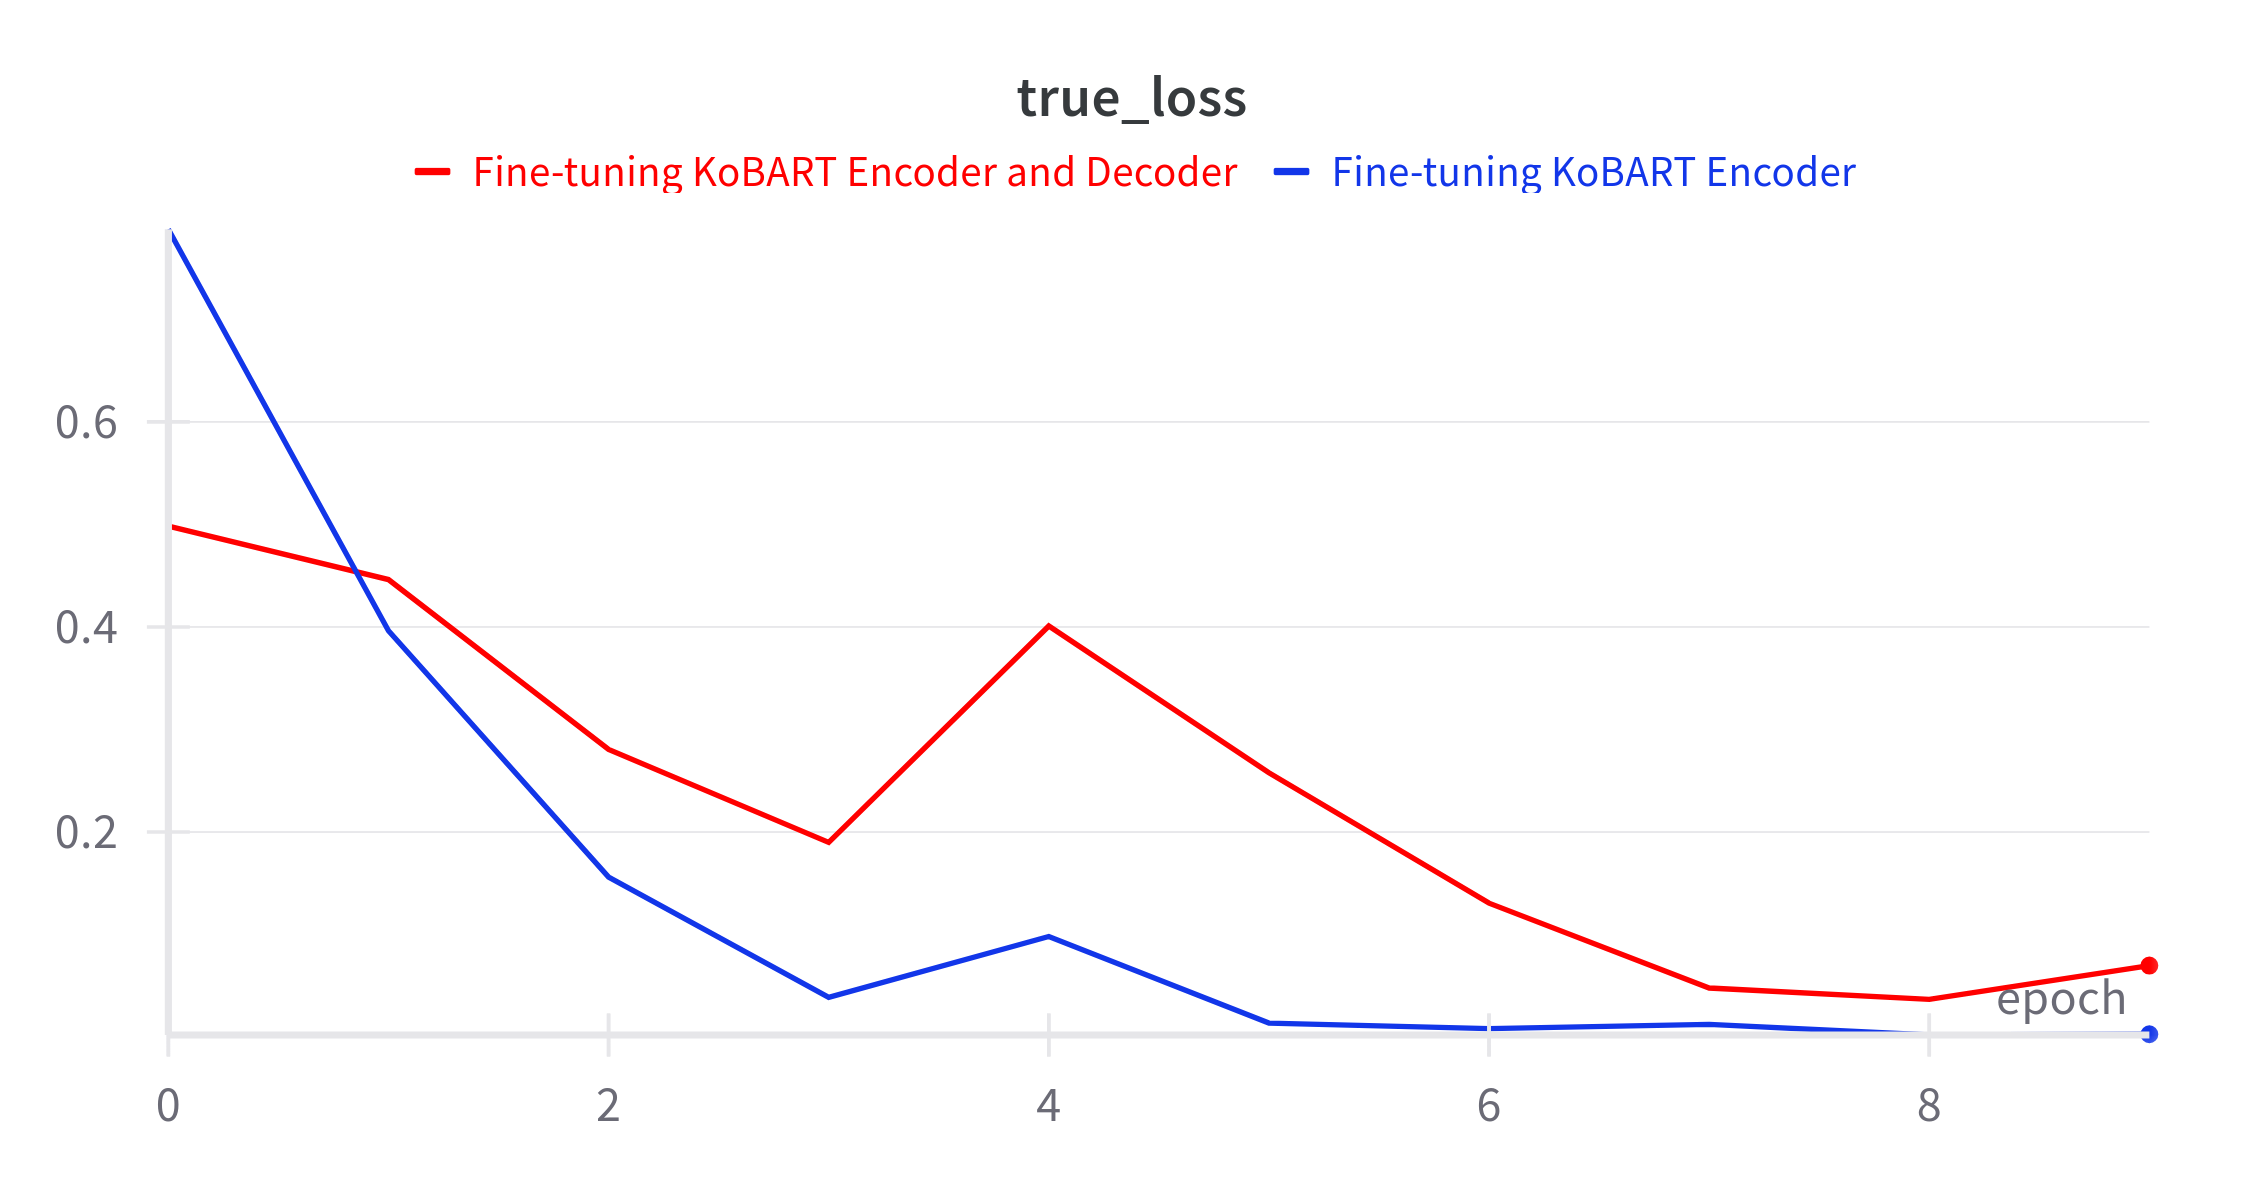
\includegraphics[width=\textwidth]{1_true_loss.png}
        \caption{True Loss}
        \label{fig:acc}
    \end{subfigure}
    \hspace{0.02\textwidth}
    \begin{subfigure}[b]{0.4\textwidth}
        \centering
        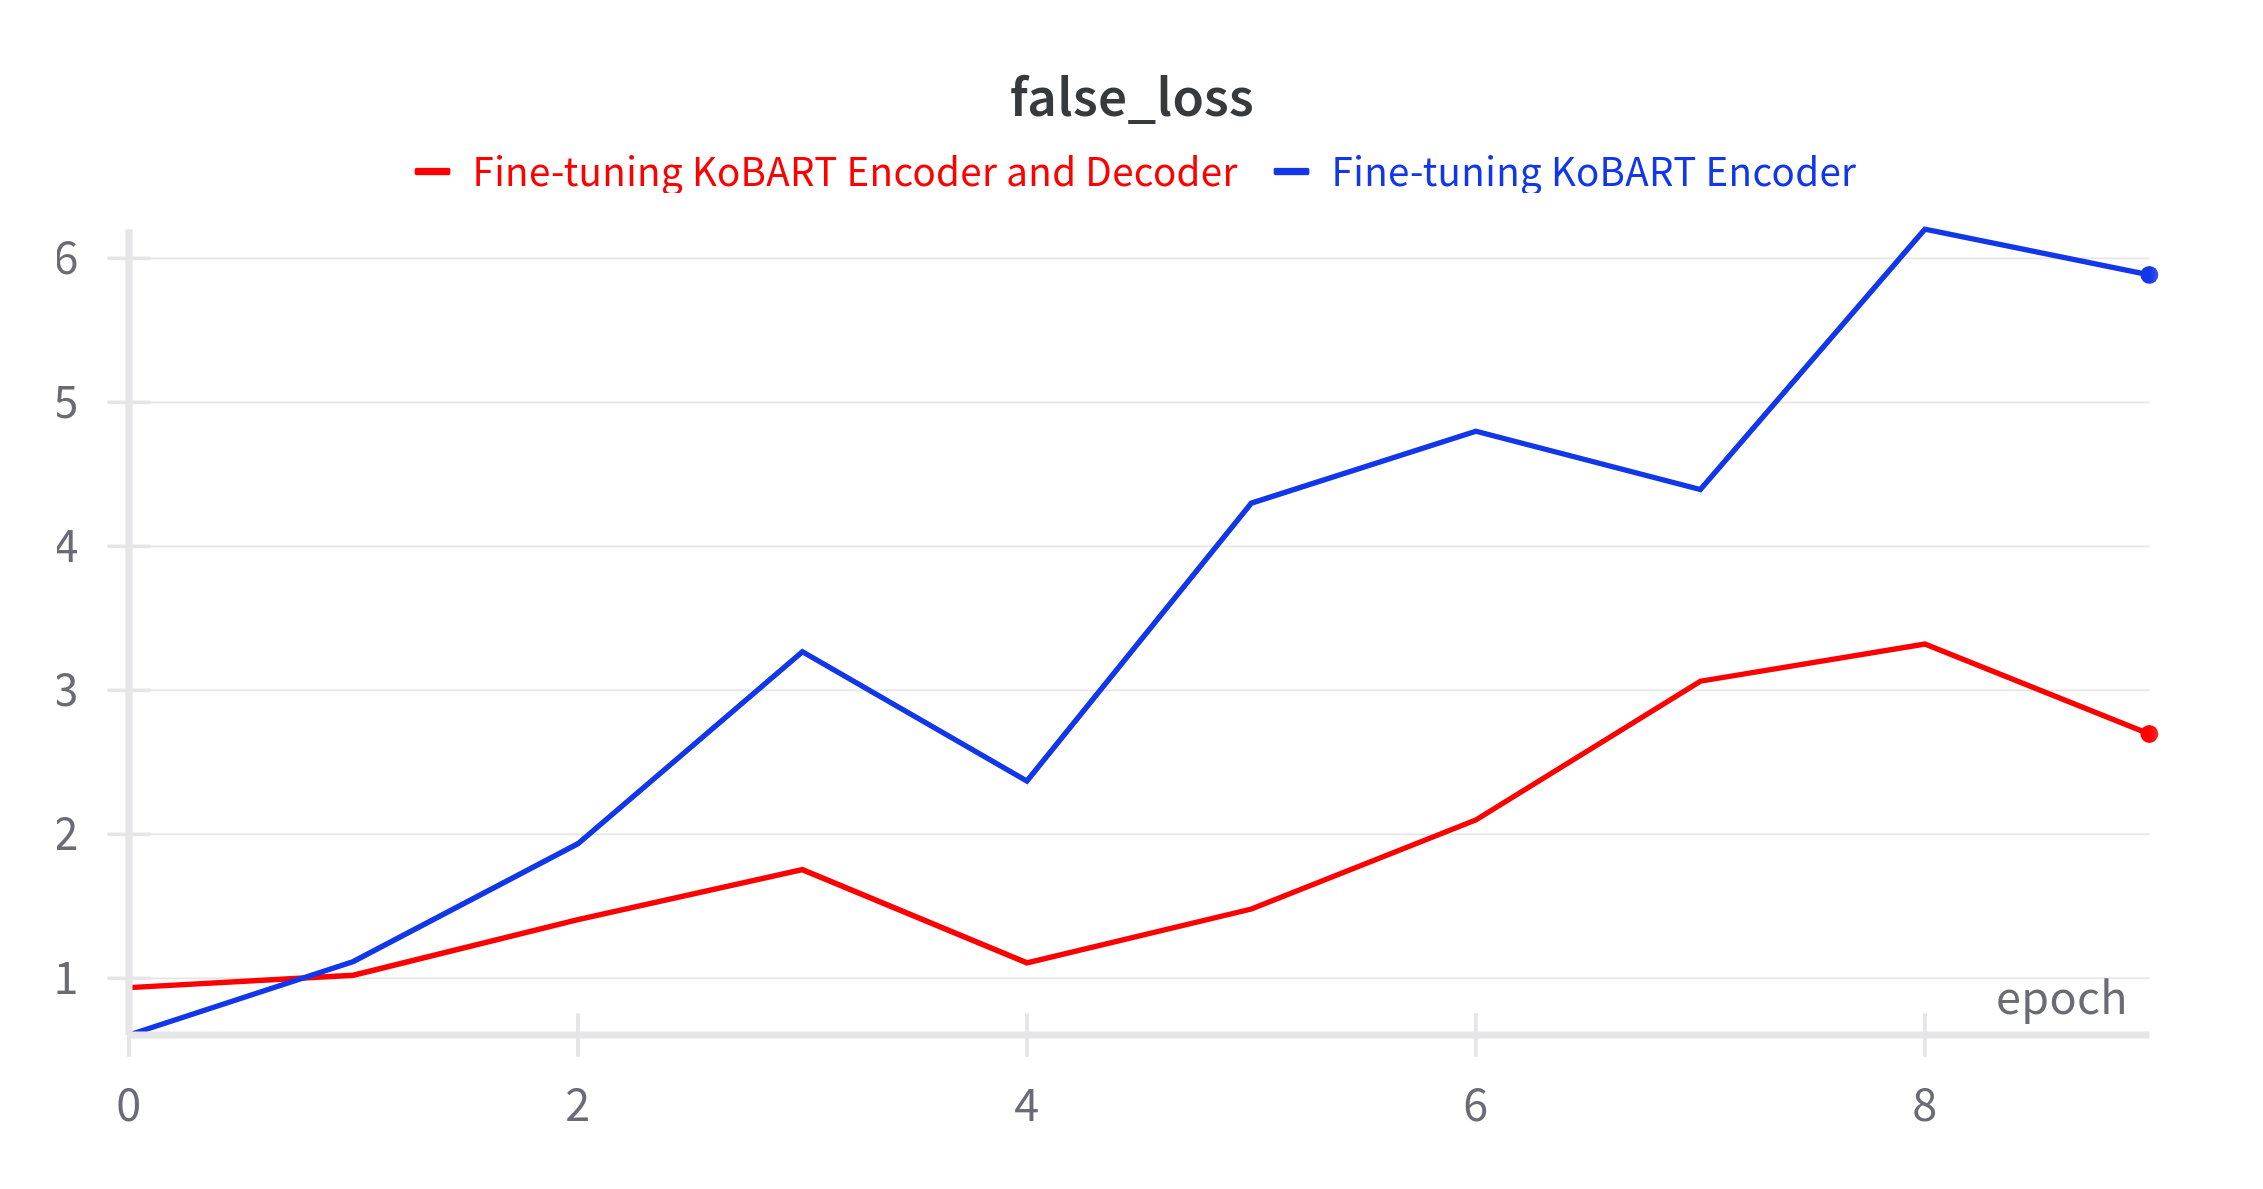
\includegraphics[width=\textwidth]{1_false_loss.png}
        \caption{False Loss}
        \label{fig:loss}
    \end{subfigure}
    
    \vspace{0.4cm}  % 그림 줄 간격 조정
    % 두 번째 줄
    \begin{subfigure}[b]{0.4\textwidth}
        \centering
        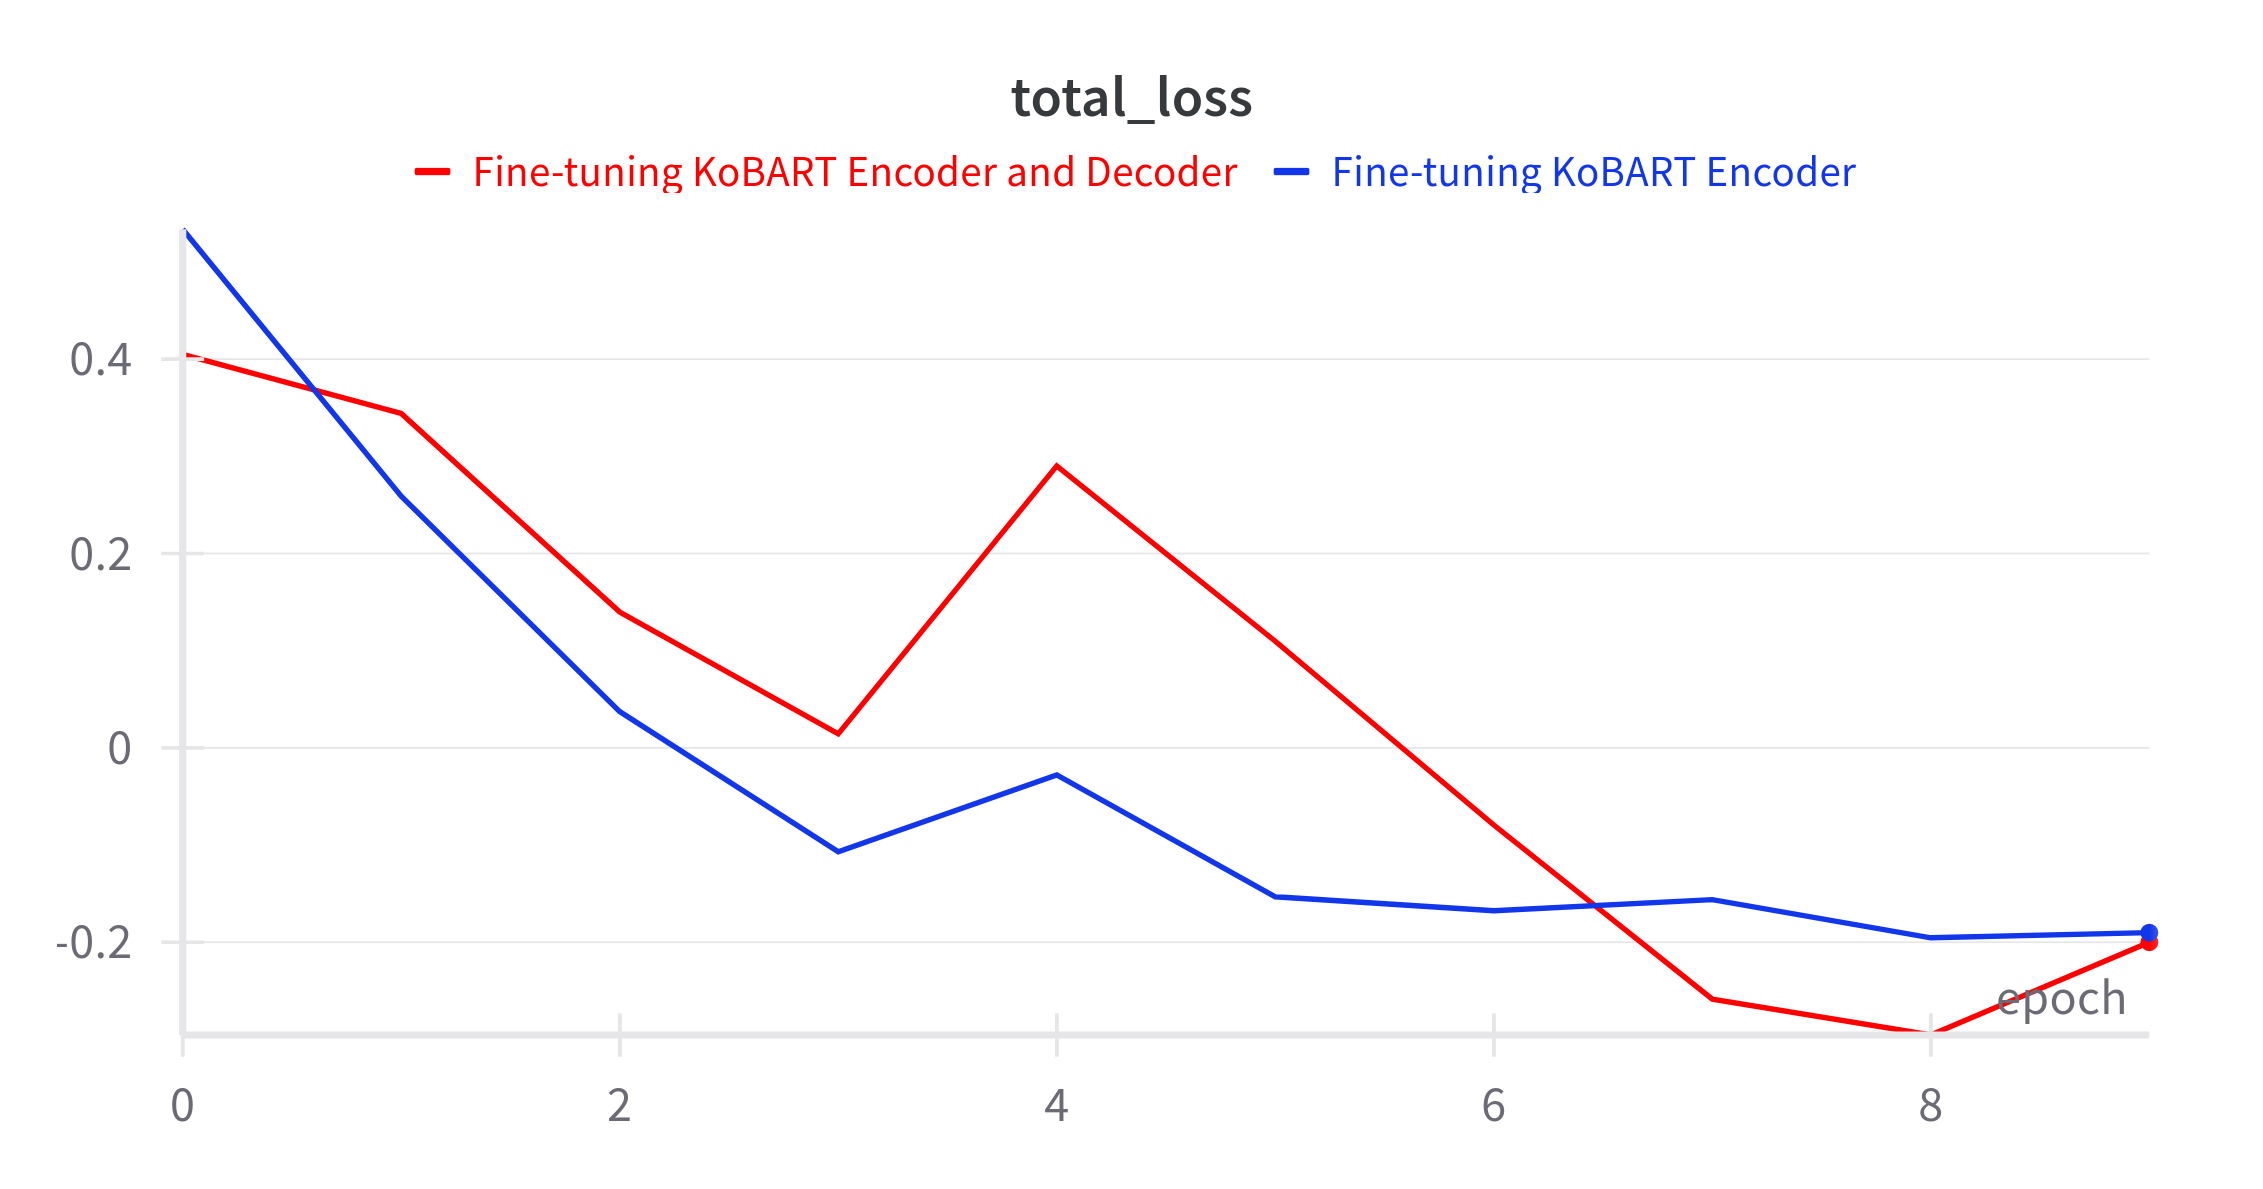
\includegraphics[width=\textwidth]{1_total_loss.png}
        \caption{Total Loss}
        \label{fig:f1}
    \end{subfigure}
    \hspace{0.02\textwidth}
    \begin{subfigure}[b]{0.4\textwidth}
        \centering
        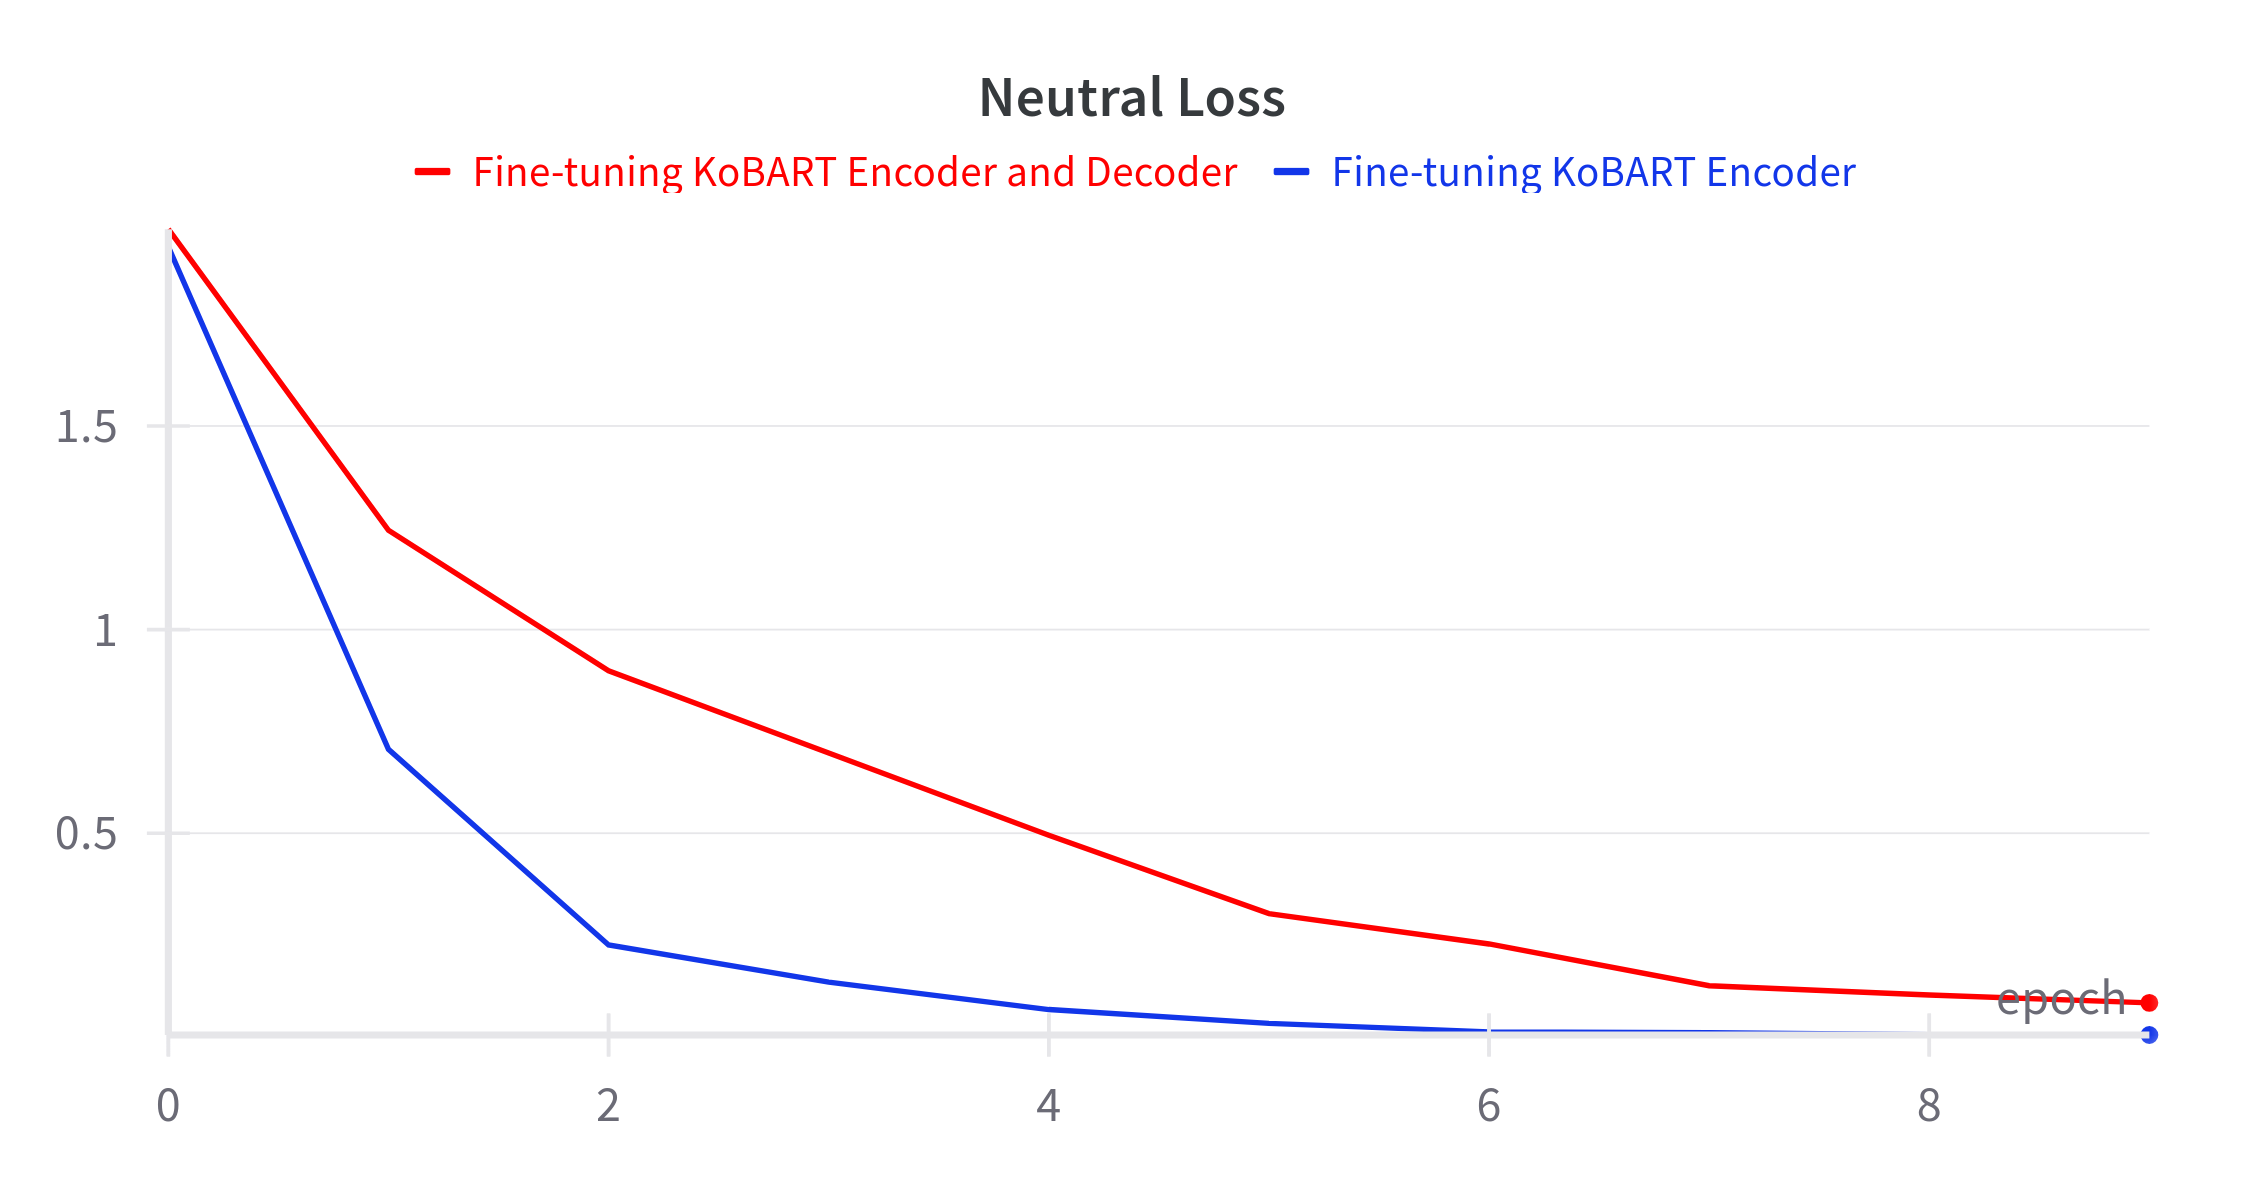
\includegraphics[width=\textwidth]{1_neutral_loss.png}
        \caption{Neutral Loss}
        \label{fig:prec}
    \end{subfigure}
    
    \caption{Decoder 포함 구조와 Encoder-only 구조의 성능 비교}
    \label{fig:performance_grid}
    \end{figure}

    실험 결과, Encoder-only 구조는 True Loss, Neutral Loss, Total Loss 항목에서 지속적으로 낮은 손실 값을 유지하였고, 학습 초기부터 더 빠른 수렴 속도를 보였다. 특히 False Loss 항목에서는 Encoder-only 모델이 상대적으로 더 높은 손실 값을 유지하였으며, 이는 기존 지식과 상충하는 예측에 대한 제거 효과가 더욱 적극적으로 발생했음을 의미한다.

    반면, 디코더를 포함한 구조는 학습 초기에 손실 값의 진동(oscillation)이 심화되었고, 후반기에는 수렴이 지연되는 불안정한 학습 양상을 보였다. 이러한 현상은 생성 기반 분류 방식이 디코더를 통한 문장 생성을 요구함에 따라, 파라미터 수가 증가하고 학습 안정성이 저하될 가능성을 시사한다.

    결과적으로, Encoder-only 구조는 입력 문장의 토큰에 대한 hidden state를 평균 풀링하여 문장 수준의 임베딩을 생성함으로써, 학습 안정성과 파라미터 효율성 측면 모두에서 우수한 성능을 나타냈다. 특히 Neutral Loss 및 Total Loss 항목에서 보다 부드럽고 안정적인 하강 곡선을 보이며, 디코더 기반 구조보다 높은 분류 안정성과 일관성을 확보하였다. 이러한 결과는 이진 분류 태스크와 같이 명시적 레이블이 존재하는 문제에서, 디코더를 활용한 문장 생성 기반 접근 방식보다 인코더 기반의 직접적인 분류 방식이 더욱 실용적이고 효율적일 수 있음을 시사한다.

   
\subsubsection{Comparison of fine-tuning performance by removing relation types}
\FloatBarrier

관계 기반 Fine-tuning의 효과를 정량적으로 검증하기 위해, 본 연구는 neutral 관계 손실과 contradiction 관계 손실을 각각 제거한 두 가지 ablation 실험을 수행하였다. 이를 통해 각 관계 유형이 모델 성능에 미치는 상대적 기여도를 분석하고자 하였다.

구체적으로, 기존의 Relation-aware Fine-tuning 구조에서 특정 관계 유형에 대응하는 손실 항목을 제거한 후, 동일한 학습 조건 하에서 모델을 fine-tuning하고, 그에 따른 성능 변화 양상을 비교 분석하였다.

각 설정은 아래와 같이 정의되며, Figure 4에서는 Model 1, Model 2, Model3으로 표기된다.

\begin{itemize}
    \item{\textbf{Model 1}:
    contradiction, neutral, entailment 관계를 모두 포함하여 full configuration으로 fine-tuning을 수행한 모델 (baseline)}
    \item{\textbf{Model 2}:
    contradiction 관계에 해당하는 손실 항목을 제외하고 neutral 및 entailment 관계만을 활용하여 fine-tuning을 수행한 모델}
    \item{\textbf{Model 3}: 
    neutral 관계에 해당하는 손실 항목을 제외하고 contradiction 및 entailment 관계만을 활용하여 fine-tuning을 수행한 모델}
\end{itemize}  

Fig 4-3는 관계 유형 제거 여부에 따라 나타나는 train loss와 accuracy 변화 추이를 시각화한 결과이다. 
\begin{figure}[htbp]
    \centering
    \begin{subfigure}[b]{0.48\textwidth}
        \centering
        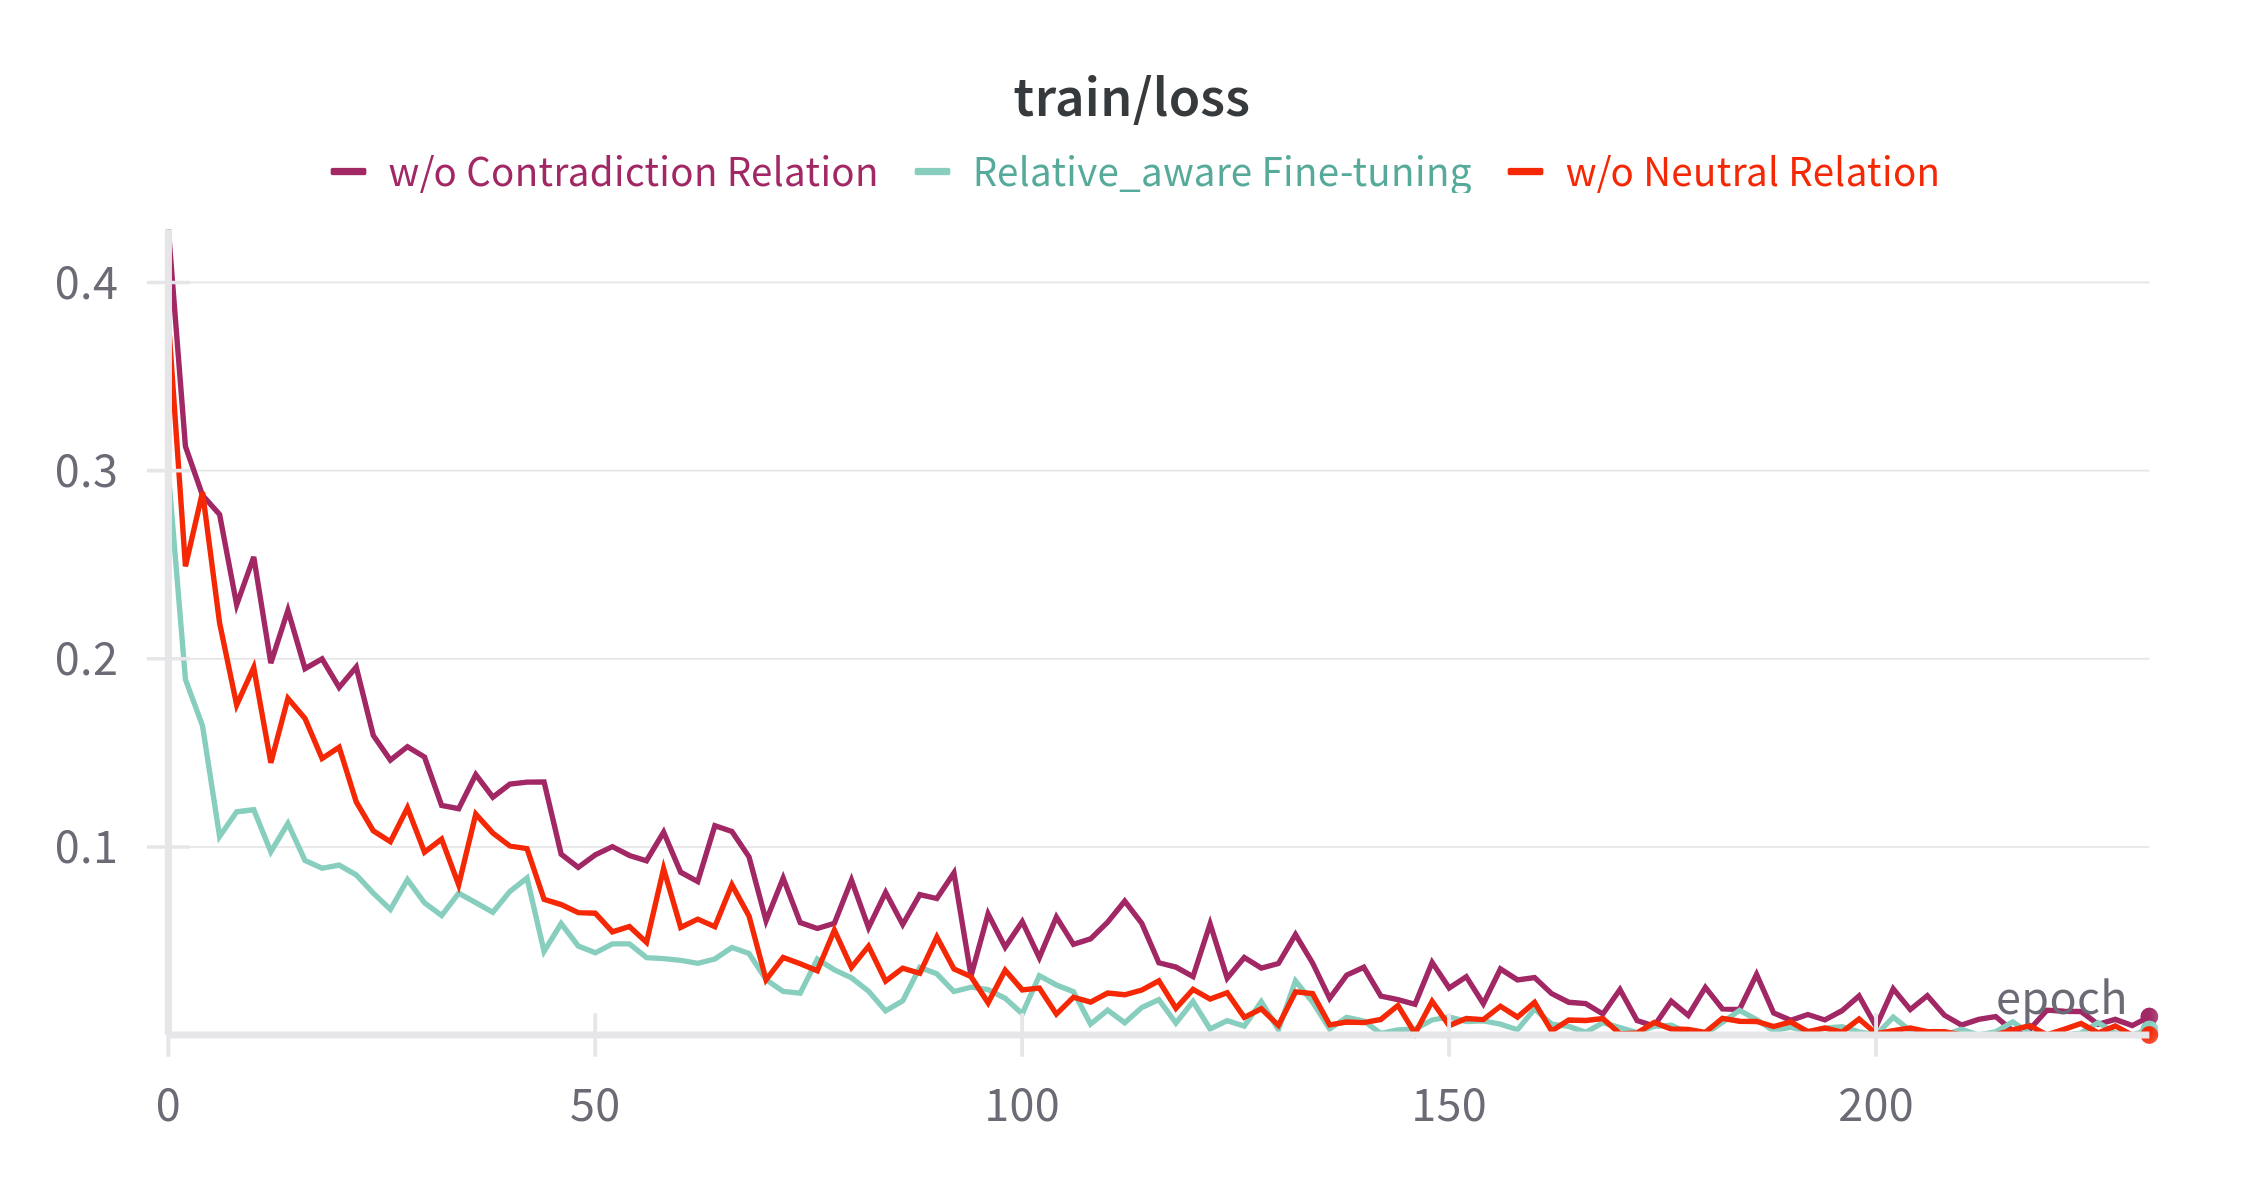
\includegraphics[width=\textwidth]{2_train_loss.png}
        \caption{Train Loss}
        \label{fig:neutral_only}
    \end{subfigure}
    \hspace{0.02\textwidth}
    \begin{subfigure}[b]{0.48\textwidth}
        \centering
        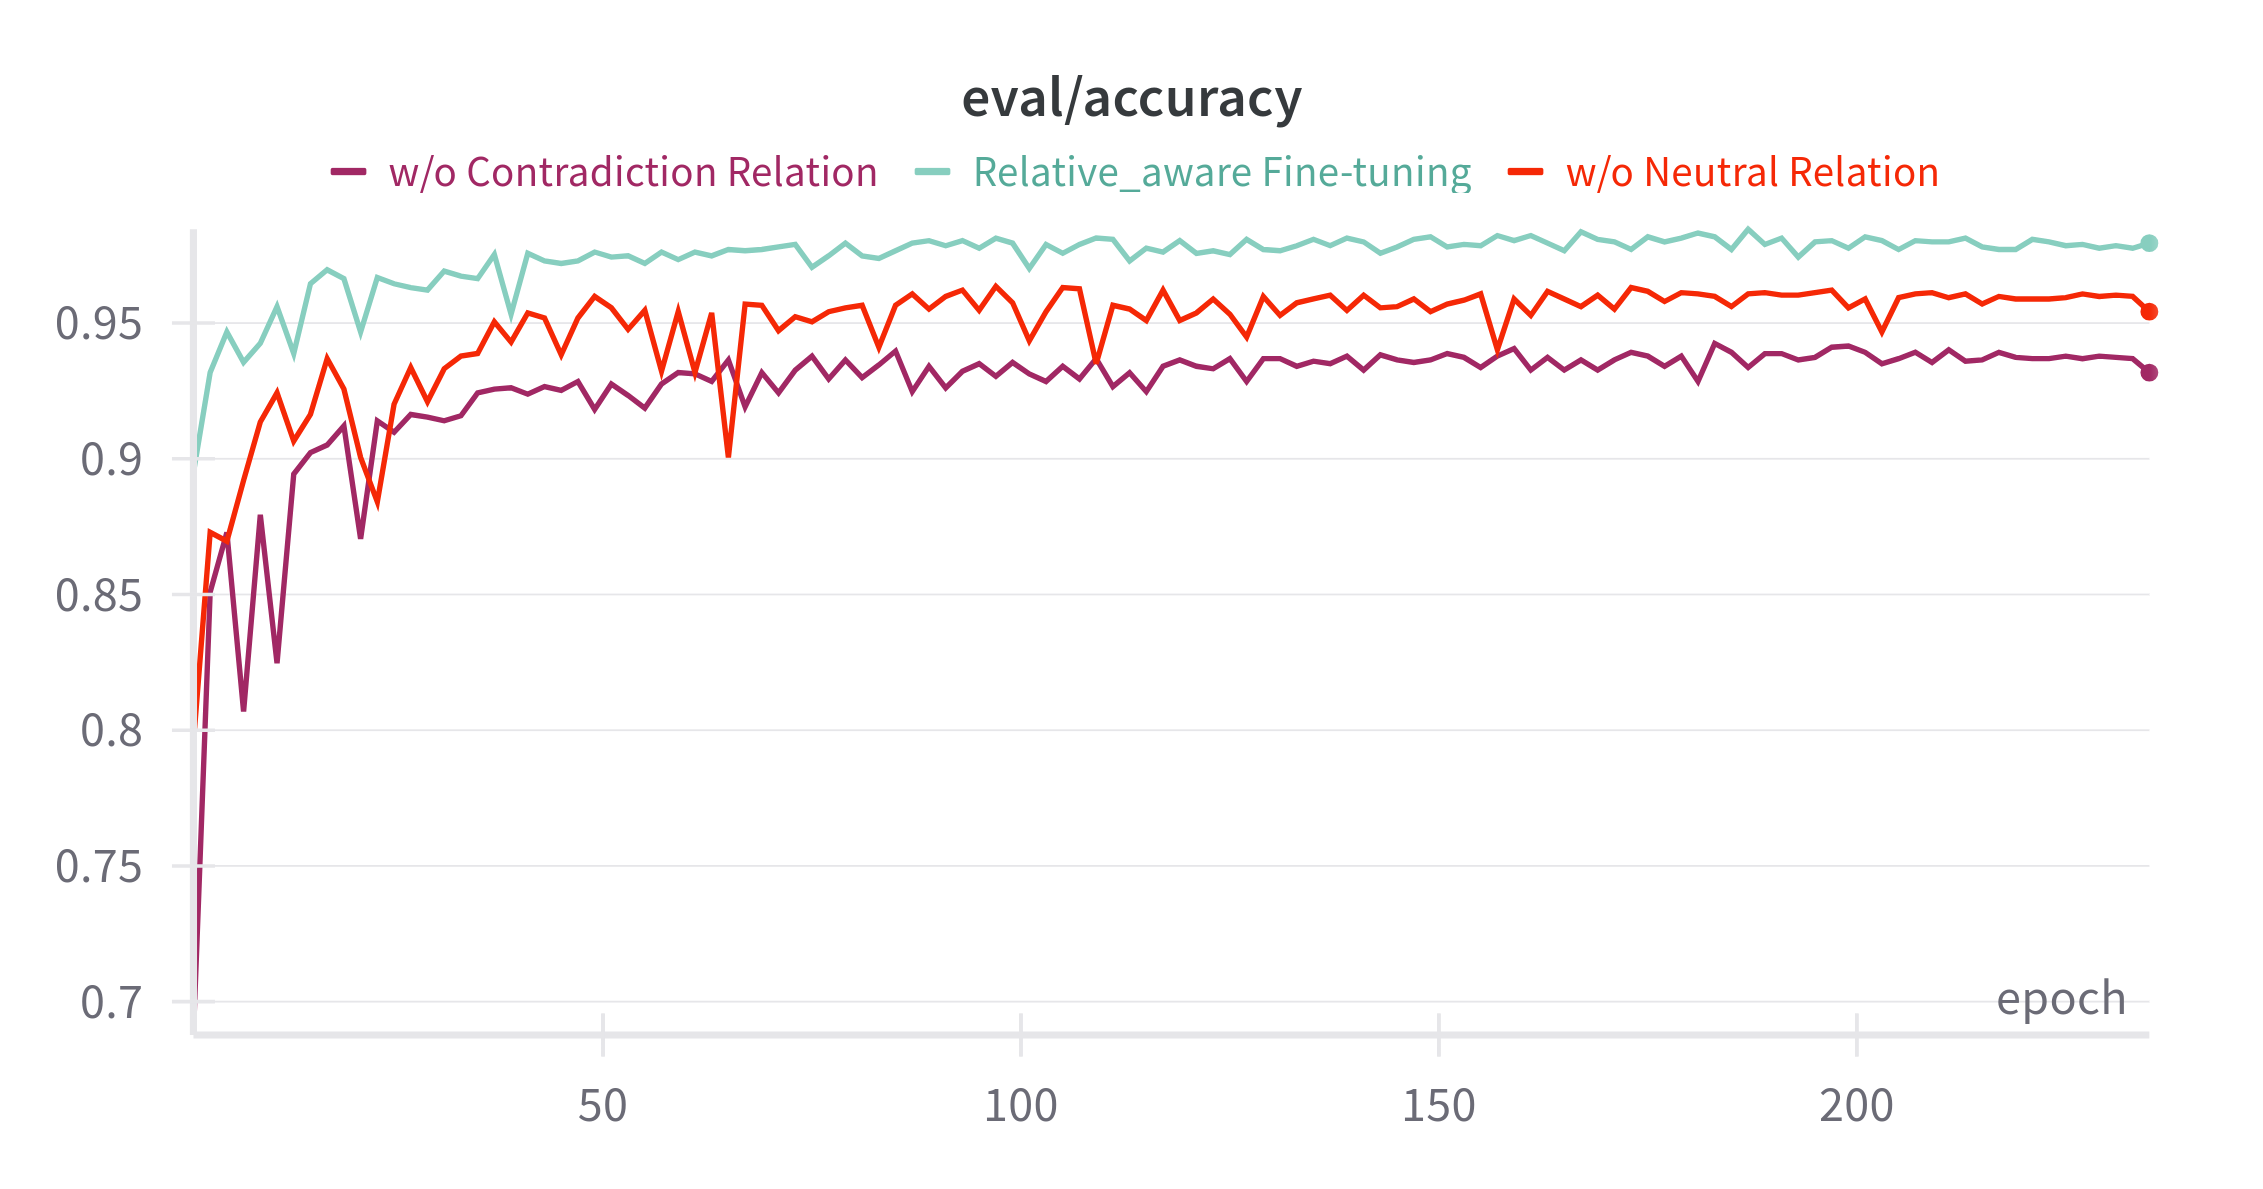
\includegraphics[width=\textwidth]{2_accuracy.png}
        \caption{Accuracy}
        \label{fig:both_relations}
    \end{subfigure}
    \caption{관계 기반 Fine-tuning에서 \texttt{neutral}, \texttt{contradiction} 손실 항목 제거에 따른 모델 성능 변화 비교.}
    \label{fig:relation_ablation}
\end{figure}

실험 결과, contradiction 손실 항목을 제외한 경우가 neutral 손실 항목을 제외한 경우보다 accuracy 하락 폭이 더 크게 나타났으며, 이는 contradiction 관계가 모델의 정보 갱신 과정에서 보다 중요한 역할을 수행함을 시사한다.

반면, 모든 관계 유형을 포함한 baseline 설정은 가장 낮은 train loss와 가장 높은 accuracy를 동시에 달성하였으며, 이는 neutral 관계와 contradiction 관계 정보가 서로 보완적으로 작용함으로써 모델의 예측 일관성과 성능을 동시에 향상시킬 수 있음을 의미한다.

결과적으로, 각 관계 유형은 상이한 방식으로 모델 fine-tuning에 기여하고 있으며, 특히 contradiction 관계는 기존 오류 지식을 제거하는 데 핵심적인 기여를 한다는 점에서 제거 시 성능 저하가 두드러진다. 이러한 분석은 Relation-aware Fine-tuning 전략 내에서 관계 유형별 손실 설계의 정당성과 실효성을 뒷받침하는 실험적 근거를 제공한다.

\subsubsection{Retrieved data comparison based on the presence of a cross-encoder}

FAISS 기반 벡터 검색은 고차원 임베딩 공간에서의 거리 기반 유사도 계산을 통해, 입력 쿼리와 의미적으로 유사한 문장을 빠르게 검색할 수 있는 효율적인 검색 방식이다. 그러나 이 방식은 주로 문장 임베딩 간의 L2 거리 또는 코사인 유사도에 의존하기 때문에, 문맥 수준에서의 정밀한 의미 일치나 논리적 관계성까지는 충분히 반영하지 못하는 한계가 존재한다.

이러한 단점을 보완하기 위해, 본 연구는 FAISS 검색 결과를 Cross-Encoder 기반 재랭킹 모델에 추가적으로 통과시켜, 쿼리 문장과 후보 문장 간의 **의미적 정합성(semantic consistency)을 더욱 정밀하게 평가하는 절차를 도입하였다. Cross-Encoder는 문장 쌍을 입력으로 받아, 두 문장 간의 상호작용을 Transformer 기반으로 직접 모델링함으로써, 단순한 벡터 유사도에 비해 문맥적 일관성과 논리적 연관성을 훨씬 정교하게 판단할 수 있다.

실험 결과, Cross-Encoder를 적용한 경우 쿼리 문장의 핵심 의미와 논리적으로 밀접한 문장들이 우선순위 상위에 재정렬되는 경향을 나타냈으며, 이는 downstream task인 NLI 관계 분류 및 selective fine-tuning의 정확도 향상에 크게 기여하였다. 예를 들어, “국내 백신을 해외에 다 빼앗길 판”과 같은 쿼리에 대해 FAISS 단독 검색은 단순히 “백신 관련” 키워드를 포함한 일반적인 문장을 상위로 반환한 반면, Cross-Encoder를 적용한 경우 “백신 수급 불균형”이나 “해외 공급 압박” 등 논리적으로 밀접한 문장이 최상위에 위치하였다.

이러한 결과는 Cross-Encoder가 검색 결과의 잡음을 제거하고 정밀도를 향상시키는 데 있어 필수적인 역할을 수행함을 시사한다. 특히, 본 시스템은 NLI 기반 관계 분류 및 selective fine-tuning 전략을 채택하고 있기 때문에, 검색된 문장과 쿼리 문장 간의 정밀한 의미 정합성이 전체 시스템의 성능을 좌우하는 핵심 요인이 된다. 따라서 Cross-Encoder는 단순한 부가 모듈이 아닌, 시스템 품질을 결정짓는 필수 요소로 간주된다.

이와 같은 정성적 개선은 %table에 제시된 실제 검색 예시를 통해 직관적으로 확인할 수 있다. Cross-Encoder 적용 시, 쿼리 문장과 의미적 유사성이 높은 문장들이 상위에 위치하며, 단순 벡터 기반 검색 결과보다 훨씬 문맥 정합성 높은 결과를 제공함을 확인할 수 있다.
    \renewcommand{\arraystretch}{1.35}
    \begin{table}[H]
    \caption{Cross-Encoder 적용 여부에 따른 Retrieve 문장 비교 예시}
    \label{tab:retrieval-results}
    \centering
    \small
    \begin{tabularx}{\textwidth}{>{\raggedright\arraybackslash}p{3.7cm}X
                                        S[table-format=1.3]
                                        S[table-format=1.3]}
    \toprule
    \textbf{Query} & \textbf{Retrieved Sentence} & \textbf{Sim. Score} & \textbf{Re-rank Score} \\
    \midrule
    
    \multirow{3}{=}{\textbf{국내 백신을 해외에 다 빼앗길 판}} 
    & 백신 개발돼도 해외에 다 뺏길 판…불만 쌓일 대로 쌓였다 & 0.790 & 0.611 \\
    & 백신 선택권이 없어 중국산 백신 맞는다 & 0.781 & 0.400 \\
    & 한국만 백신 선택권이 없다 & 0.772 & 0.312 \\
    \midrule
    
    \multirow{3}{=}{\textbf{불가리스가 코로나19에 효과}} 
    & 불가리스가 코로나 19를 77.8\% 수준으로 억제하는 효과 분석 & 0.812 & 0.730 \\
    & 방역 수준은 에탄올만큼 떨어져 죽는 것으로 추정 & 0.811 & 0.188 \\
    & 노바백스의 코로나19 백신 후불보급 & 0.813 & 0.177 \\
    \midrule
    
    \multirow{3}{=}{\textbf{AZ백신은 국내 허가됨}} 
    & 노바백스 백신은 인허가를 통해 도입 계획임 & 0.867 & 0.433 \\
    & 계약은 비밀유지협약과 함께 진행됨 & 0.847 & 0.358 \\
    & 스푸트니크V 백신 도입 추진 중 & 0.858 & 0.271 \\
    \midrule
    
    \multirow{3}{=}{\textbf{머리카락이 코로나를 옮긴다}} 
    & 머리카락이 신종 코로나 바이러스를 옮긴다 & 0.844 & 0.870 \\
    & 비타민 C를 먹으면 도움이 된다는 주장 & 0.806 & 0.191 \\
    & 마스크 내 화학물질이 폐암 유발할 수 있다 & 0.792 & 0.169 \\
    \bottomrule
    \end{tabularx}
    \end{table}
   

\subsubsection{Performance comparison based on contradiction loss design}

본 연구에서는 모델이 기존 지식을 효과적으로 제거할 수 있도록 유도하는 손실 항목인 Contradiction Loss의 설계 방식이 전체 학습 성능에 미치는 영향을 정량적으로 비교하였다. 이를 위해 총 네 가지 손실 함수 조합을 정의하고, 각 실험 설정의 차이를 Table 4-6에 정리하였다. 비교의 핵심 목적은 False Loss가 모델의 잘못된 기존 판단을 얼마나 효과적으로 제거하도록 유도하는지를 확인하고, True Loss와의 균형을 어떻게 조정할 것인지에 대한 실험적 근거를 확보하는 데 있다.

\begin{table}[H]
    \centering
    \renewcommand{\arraystretch}{1.3}
    \caption{Contradiction Loss 구성 방식별 총합 손실 함수 정의}
    \label{tab:loss-designs}
    \begin{tabularx}{\textwidth}{>{\raggedright\arraybackslash}p{1.2cm}X}
        \toprule
        \textbf{Case} & \textbf{Total Loss 정의} \\
        \midrule
        (1) & \( \mathcal{L} = \log(\text{True Loss}) + \log(\text{False Loss}) \) \\
        (2) & \( \mathcal{L} = \log(\text{True Loss}) - \log(\text{False Loss}) \) \\
        (3) & \( \mathcal{L} = \log(\text{True Loss}) - \alpha \cdot \log(\text{False Loss}) \quad (\alpha = 0.5) \)\\
        (4) & \( \mathcal{L} = \log(\text{True Loss}) - \alpha \cdot \log(\text{False Loss}) \quad (\alpha = 0.1) \) \\
        \bottomrule
    \end{tabularx}
\end{table}
   
실험 결과는 다음과 같다.

\begin{figure}[htbp]
    \centering

    \begin{subfigure}[b]{0.48\textwidth}
        \centering
        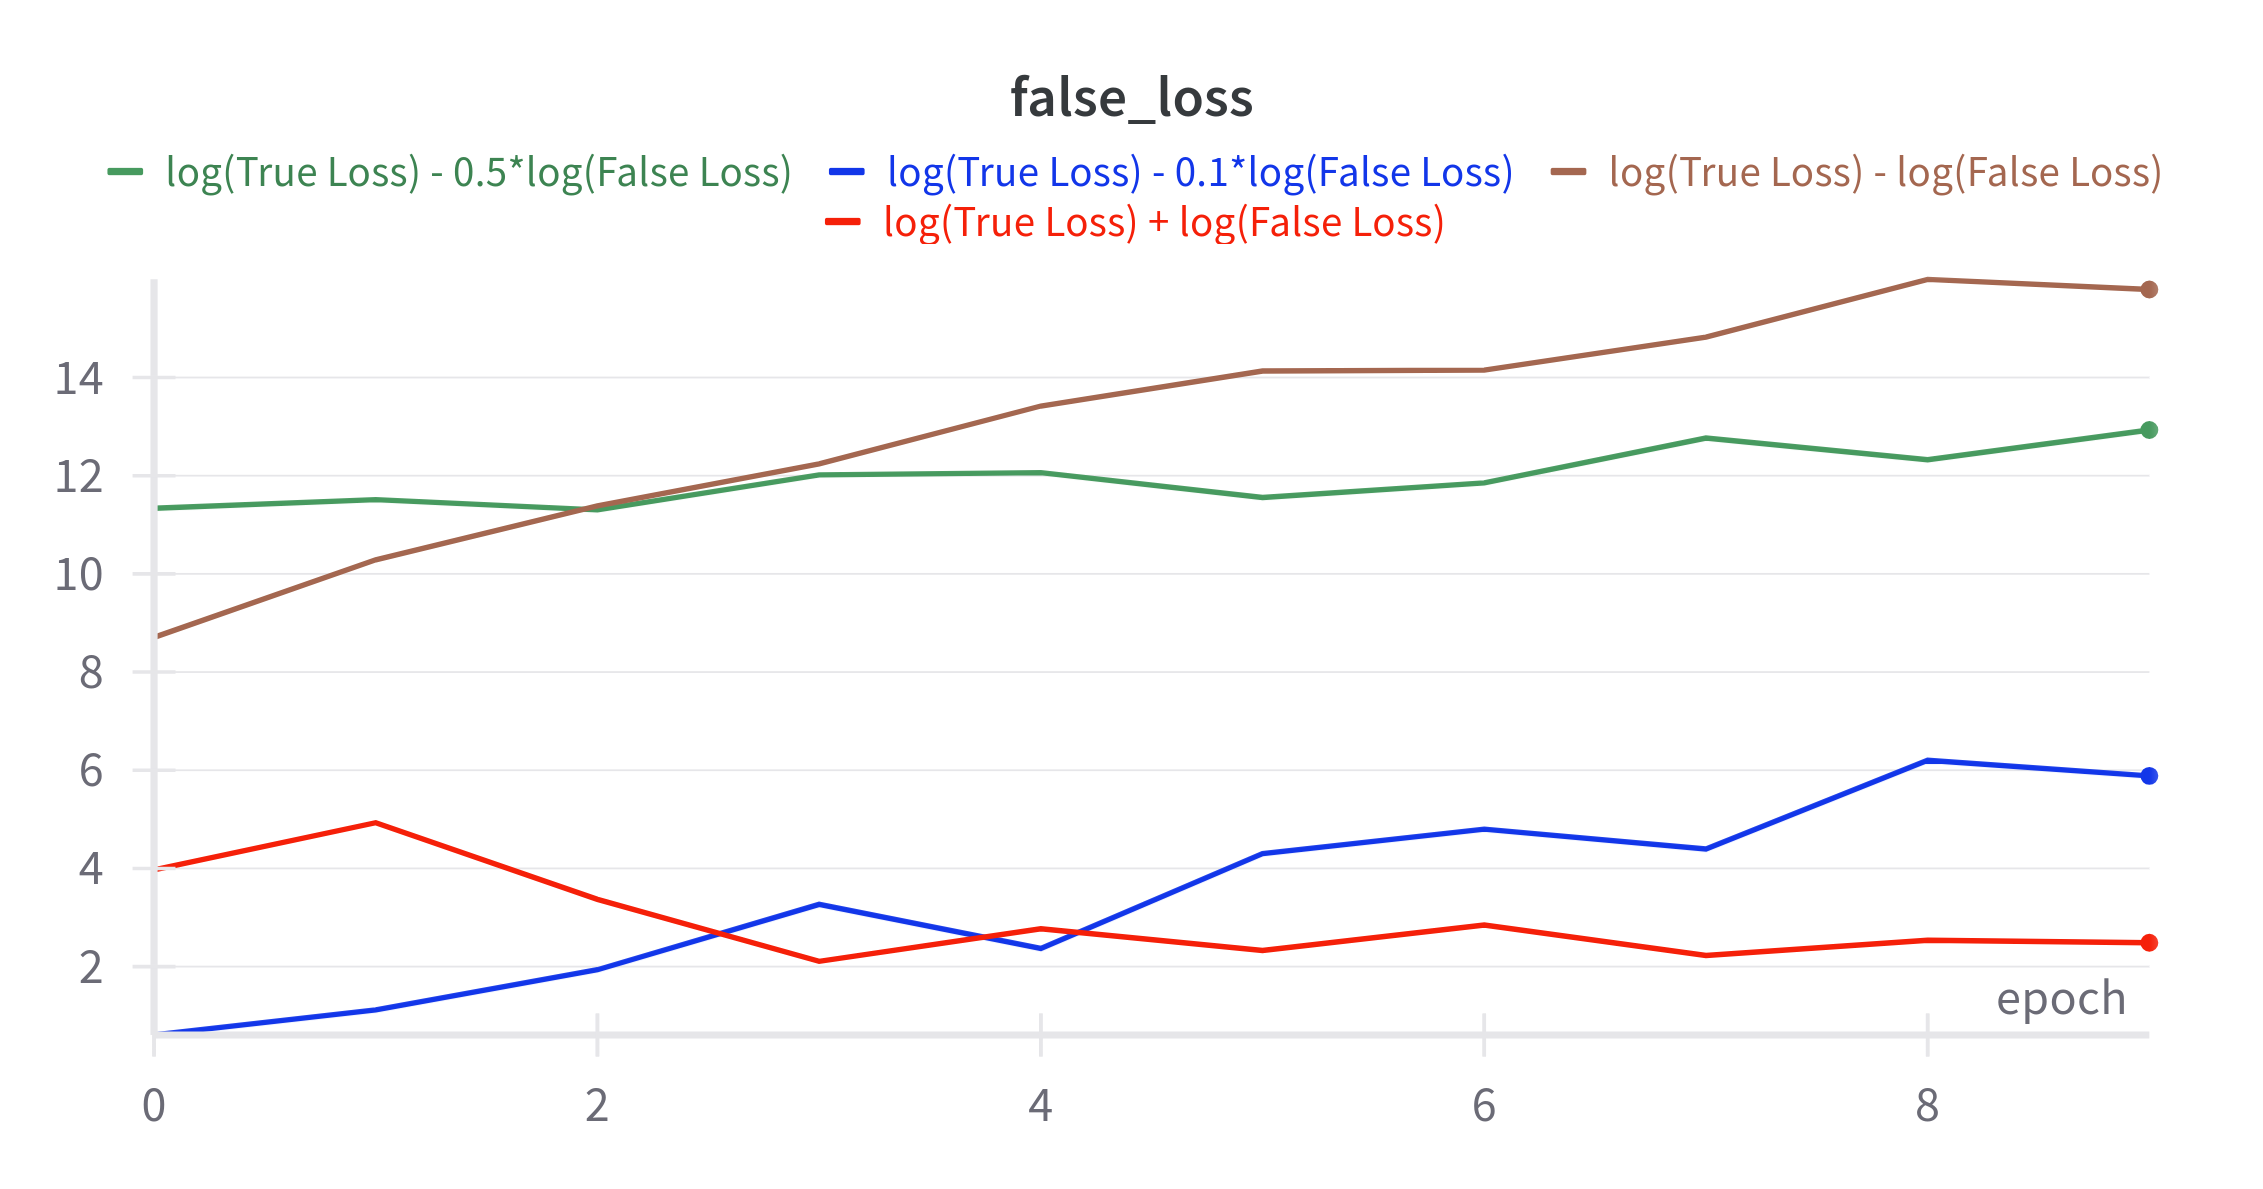
\includegraphics[width=\textwidth]{3_false_loss.png}
        \caption{Train Loss}
        \label{fig:neutral_only}
    \end{subfigure}
    \hspace{0.02\textwidth}
    \begin{subfigure}[b]{0.48\textwidth}
        \centering
        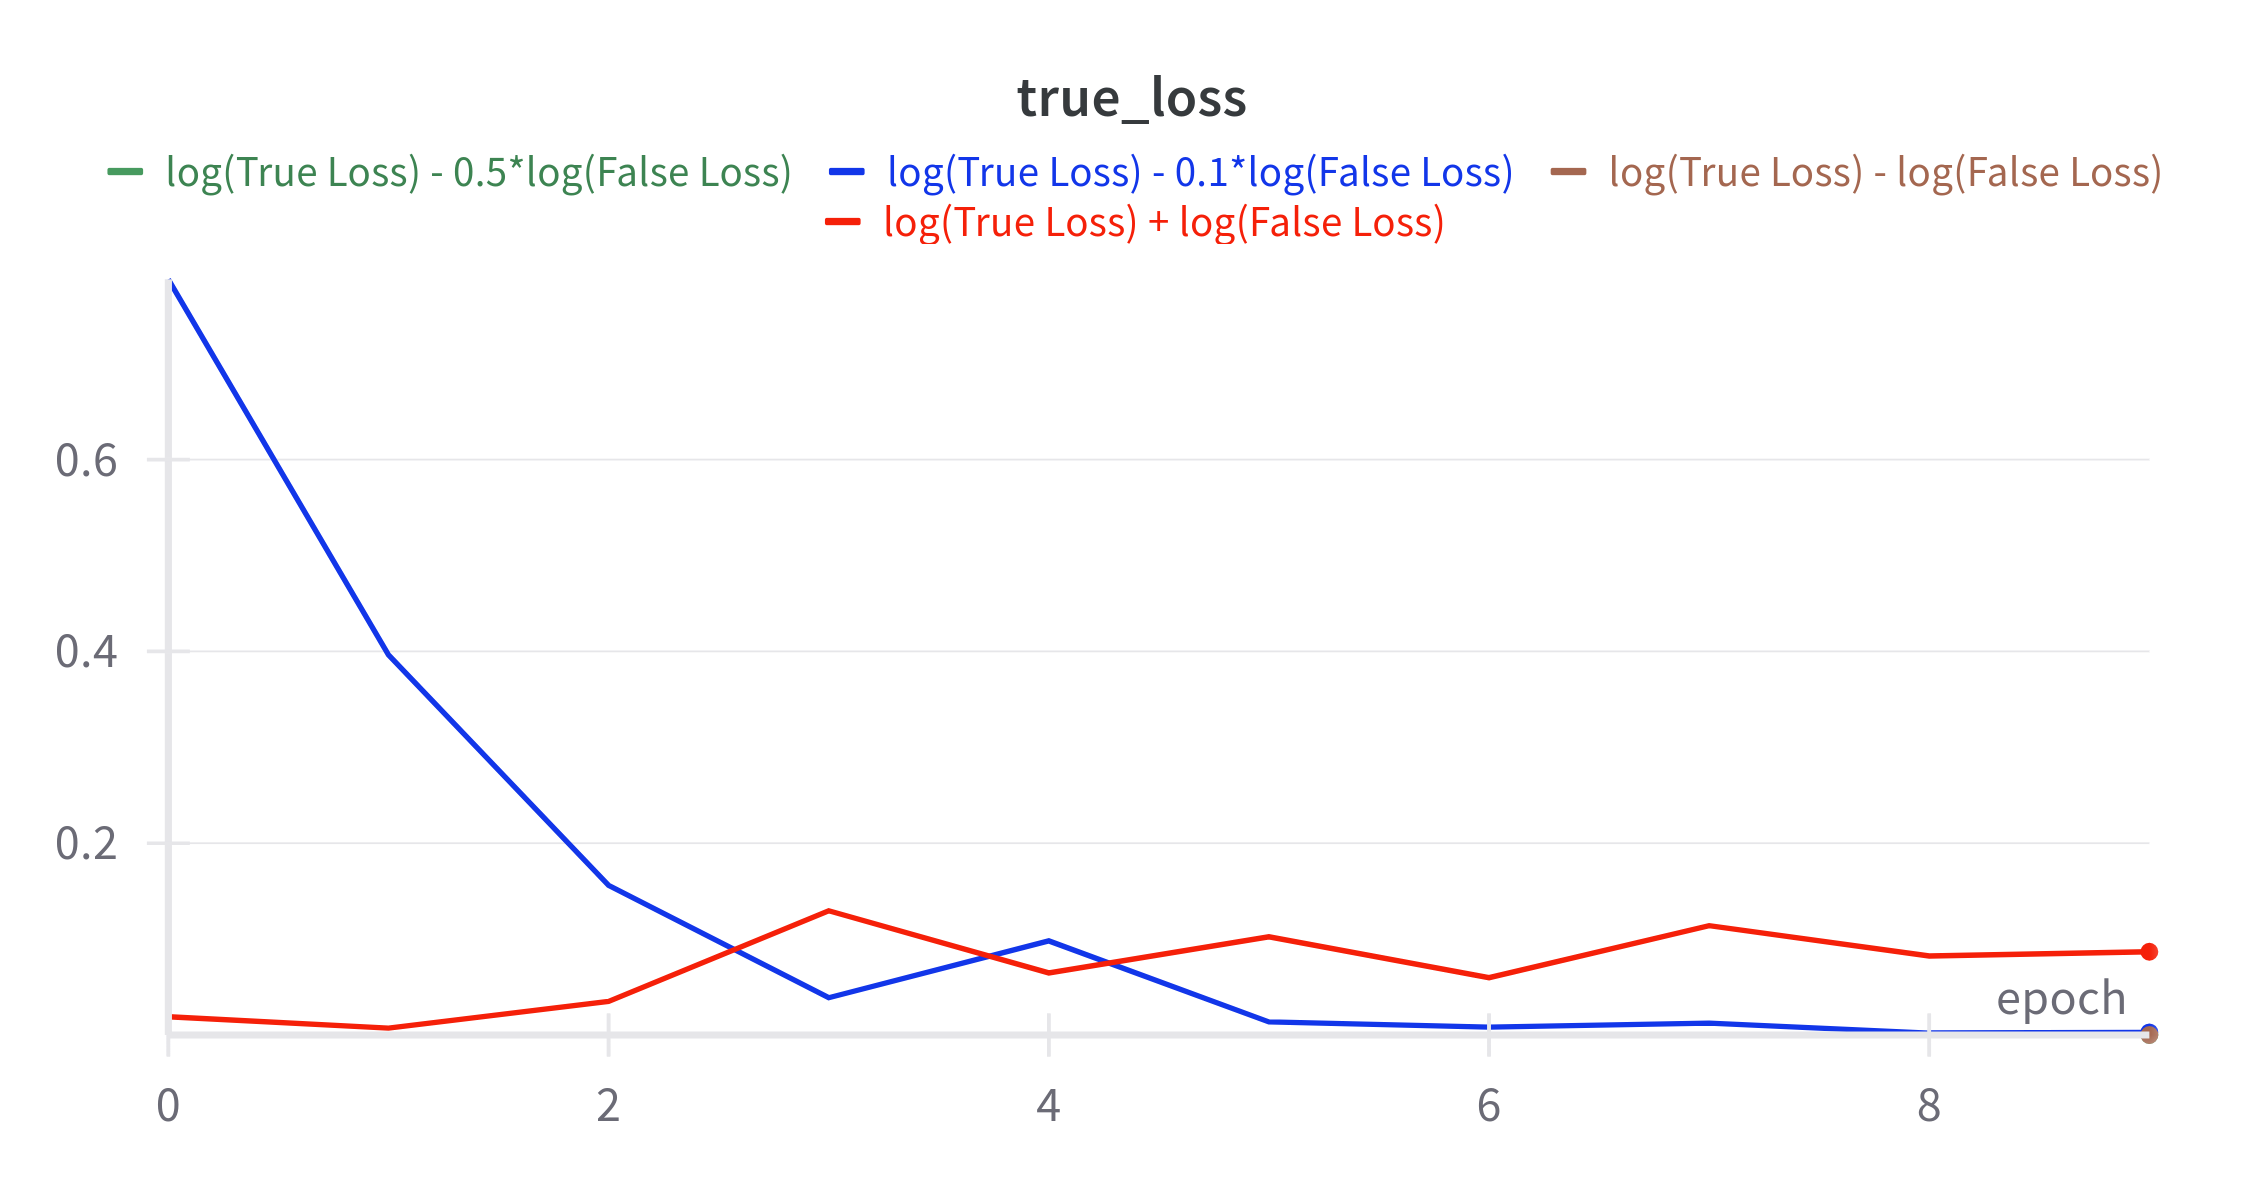
\includegraphics[width=\textwidth]{3_true_loss.png}
        \caption{Accuracy}
        \label{fig:both_relations}
    \end{subfigure}
    \hspace{0.02\textwidth}
    \begin{subfigure}[b]{0.48\textwidth}
        \centering
        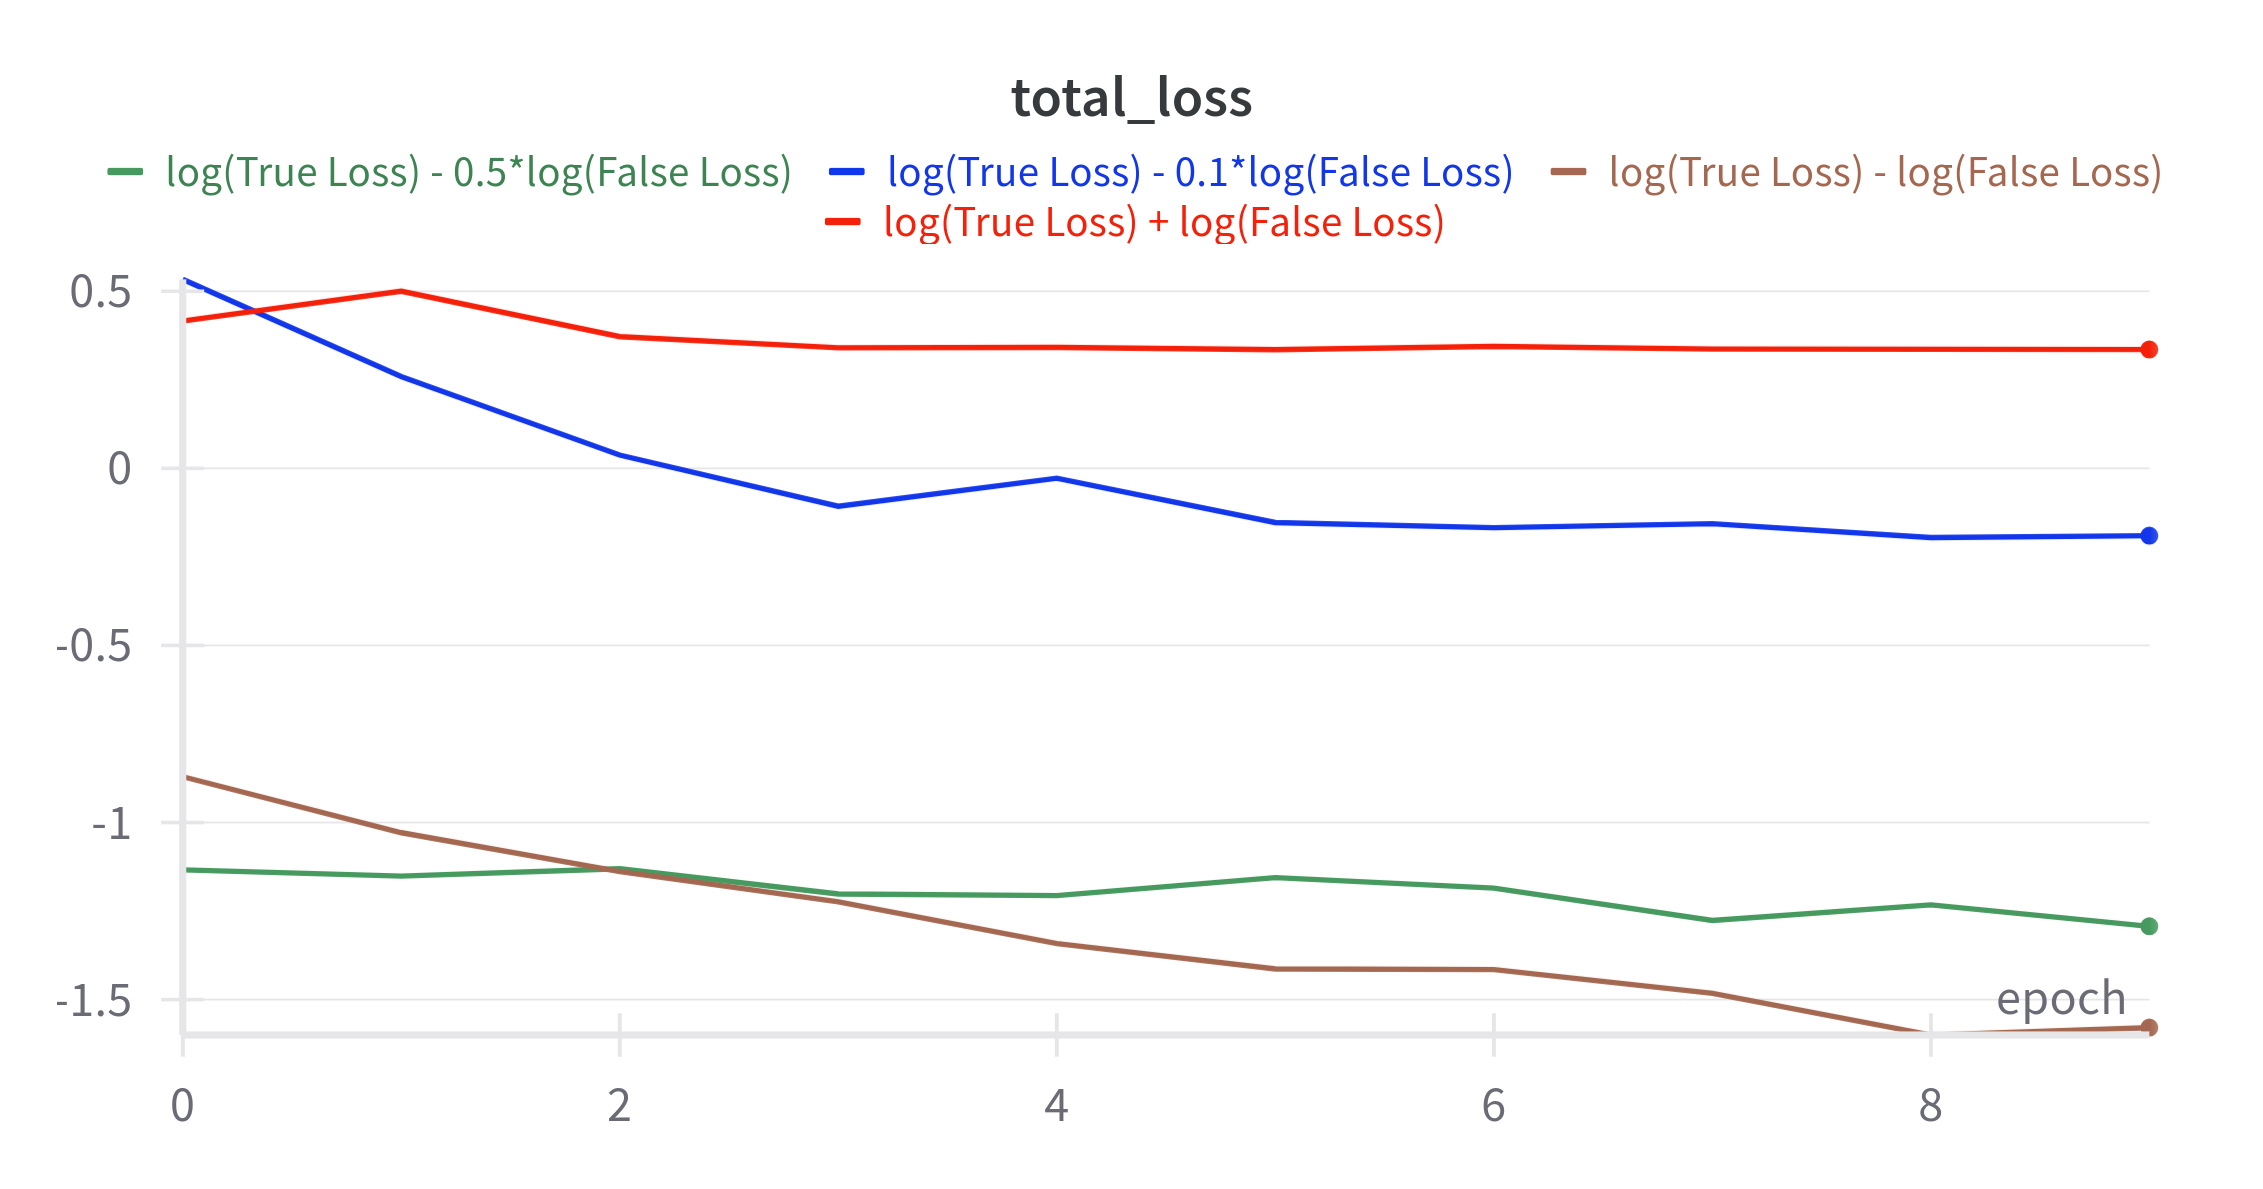
\includegraphics[width=\textwidth]{3_total_loss.png}
        \caption{Accuracy}
        \label{fig:both_relations}
    \end{subfigure}
    \caption{contradiction loss 설계에 따른 성능어떤 걸 써야 학습이 되는가에 대한 비교}
    \label{fig:relation_ablation}
\end{figure}

\begin{itemize}
    \item \textbf{Case (1)}의 경우, False Loss가 학습이 진행됨에 따라 오히려 감소하는 역효과가 나타났으며, 이는 모델이 contradiction 관계에 해당하는 기존 오류 정보를 보존하려는 경향을 보였음을 시사한다.
    
    \item \textbf{Case (2)}와 \textbf{Case (3)}는 False Loss 항목의 영향력이 과도하게 커진 결과, Total Loss가 음수 방향으로 빠르게 수렴하였고, True Loss는 학습 초기에 0 부근에서 정체되며 더 이상 감소하지 않는 비정상적인 학습 양상이 발생하였다. 이는 False Loss의 과도한 가중치가 모델의 일반적인 분류 능력을 저해했음을 의미한다.
    
    \item \textbf{Case (3)}과 \textbf{Case (4)}에 대해 False Loss 항목의 가중 계수인  \(\alpha \)를 조정하여, 해당 값이 전체 학습 성능에 미치는 영향을 분석하였다. 특히  \(\alpha = 0.5\)로 설정한 Case (3)의 경우, False Loss가 학습 초반부터 약 4.0의 높은 값에서 시작하였으며, 학습이 진행되더라도 손실이 감소하지 않는 경향을 보였다. 이는 모델이 contradiction 관계에 대해 지나치게 강한 패널티를 받으면서, 오히려 업데이트를 회피하거나 역효과를 발생시키는 현상으로 해석된다. 뿐만 아니라, 동일한 설정 하에서 True Loss 및 Total Loss 또한 수렴하지 않고 정체되는 양상이 관찰되었으며, 이는 과도한 False Loss 가중치가 전체 학습 과정을 방해함을 보여준다. 반면, \(\alpha = 0.1\)을 적용한 Case (4)의 경우, 모든 손실 항목이 안정적으로 변화하면서 바람직한 학습 곡선을 형성하였다.
    
\end{itemize}
    
이러한 결과는, 값의 미세한 조정만으로도 학습 안정성에 큰 영향을 미칠 수 있음을 시사하며, 모델 편집을 위한 Contradiction Loss 설계 시 가중 계수의 정교한 튜닝이 필수적임을 보여준다. 본 연구에서는 별도의 자동 최적화 절차 없이, 실험적 관찰을 바탕으로 을 수동으로 설정하였으며, 해당 값이 실용적인 기준선으로서 안정적인 성능을 확보함을 확인하였다.

\subsubsection{Comparative analysis of encoder fine-tuning strategies}

Relation-aware Fine-Tuning의 파라미터 효율성과 학습 안정성을 분석하기 위해, Encoder 전체를 fine-tuning하는 방식(이하 Case (1)) 과 Encoder 내부의 MLP Layer만을 선택적으로 fine-tuning하는 방식(이하 Case (2)) 간의 성능 차이를 비교하였다.

실험 결과, Encoder의 MLP Layer만을 fine-tuning한 설정이 Encoder 전체를 fine-tuning한 경우보다 더 낮은 loss 값과 더 빠른 수렴 속도를 보였다. 특히 total loss 기준으로 초기 epoch에서부터 빠르게 감소하는 경향을 나타냈으며, 학습 후반까지도 안정적인 손실 곡선을 유지하였다. 반면, Encoder 전체를 fine-tuning한 경우는 loss 곡선이 불안정하게 진동하거나 수렴 속도가 느려지는 양상을 보였으며, 이는 불필요한 파라미터 업데이트가 모델의 기존 표현 구조를 훼손했을 가능성을 시사한다.

또한, 학습 시간과 연산 자원 측면에서도 MLP Layer만을 fine-tuning한 방식이 훨씬 효율적인 결과를 보였다. 전체 파라미터 수 대비 업데이트 대상 파라미터 비율이 작아 GPU 메모리 사용량과 연산 부하가 줄었고, 학습 시간 역시 전체 fine-tuning 대비 약 35\% 이상 단축되었다. 이러한 결과는 Relation-aware Fine-Tuning이 요구하는 구조적 선택성과 모델의 안정성 확보 측면에서, 불필요한 파라미터 업데이트를 최소화하고 핵심 정보에만 집중하는 것이 오히려 성능 향상에 기여할 수 있음을 실증적으로 보여준다.

결론적으로, 본 연구는 Encoder 전체를 fine-tuning하는 전통적 접근보다, 표현 학습의 핵심 경로인 MLP Layer만을 제한적으로 수정하는 방식이 분류 안정성, 학습 효율성, 자원 절감 측면 모두에서 더 효과적임을 입증하였으며, 이는 향후 대규모 모델을 실용적으로 편집 및 유지하기 위한 효율적 접근 방식으로 제안될 수 있다.

\subsection{Performance Comparison}

\subsubsection{Performance comparison by dataset configuration}

본 절에서는 학습에 사용된 데이터 구성 방식에 따라 Relation-aware Fine-Tuning의 성능이 어떻게 달라지는지를 정량적으로 비교하였다. Table 4-7은 실험에 사용된 네 가지 데이터 구성(configuration)을 요약한 것으로, 각 구성은 학습에 활용된 데이터의 범위와 출처에 따라 다음과 같이 정의된다.

\begin{table}[htbp]
    \centering
    \caption{Dataset configurations for transfer learning.}
    \resizebox{\textwidth}{!}{%
    \begin{tabular}{lcccc}
    \toprule
    \textbf{Datasets} & \textbf{Test 1} & \textbf{Test 2} & \textbf{Test 3} & \textbf{Test 4} \\
    \midrule
    Pretraining & Old data(2019 from Kaggle)
             & +New data(Training)
             & +AI FactChecknet(Transfer data)
             & -Old data(2019 from Kaggle) \\
   
    \bottomrule
    \end{tabular}%
    }
\end{table}
%%%%%%%%%%model ? Test?
\begin{itemize}
    \item{\textbf{Test 1}:
    Old data만을 학습에 사용한 구성 (2019년 Kaggle에서 수집된 영어 기반 COVID-19 가짜 뉴스 데이터를 번역하여 사용)}
    \item{\textbf{Test 2}:
    Test 1에 New data(2021년 이후 수집된 최신 한국어 데이터)를 추가한 구성}
    \item{\textbf{Test 3}: 
    Test 2에 더해, AI FactCheckNet에서 수집된 외부 검증 데이터(Transfer data)를 추가한 구성}
    \item{\textbf{Test 4}: 
    Test 3에서 Old data를 제거한 구성 (New data와 Transfer data만을 사용)}
\end{itemize}  

각 구성은 모델이 어떤 시점의 정보에 기반해 fine-tuning 되었는지를 반영하며, 실험 목적은 데이터 출처와 시간대가 모델 성능에 미치는 영향을 분석하는 데 있다. 
%Fig 4-7은 각 데이터 구성에 따라 테스트한 모델의 Accuracy 변화를 시각화한 결과로, 구성별 정보 조합이 모델의 최종 예측 성능에 어떤 차이를 유발하는지를 비교적으로 보여준다.

학습 과정의 동적 특성 또한 각 모델 구성 간 뚜렷한 차이를 보였다. Model 1(Old data only)과 Model 4(New + Transfer without Old data)는 학습 초반 일정 수준의 성능에 도달한 이후 더 이상의 성능 향상이 관찰되지 않았으며, 이로 인해 early stopping 기준에서 정의된 patience 조건에 따라 비교적 이른 시점에서 학습이 종료되었다. 이는 해당 모델들이 초기 학습 단계에서 빠르게 수렴했다.

반면, Model 2(Old + New)와 Model 3(Old + New + Transfer)는 학습 후반까지 손실과 정확도 지표에서 소폭의 진동(oscillation)이 반복적으로 발생하였으며, 이는 모델이 새로운 정보와 기존 지식 간의 경계에서 fine-tuning을 계속 시도함에 따라 발생한 것으로 해석된다. 이러한 진동에도 불구하고 성능 향상 가능성이 관찰되었기 때문에, patience 조건에 도달하지 않고 오랜 학습이 지속되는 경향을 보였다. 이러한 차이는 학습 데이터 구성에 따라 모델이 새로운 정보에 반응하고 내부 파라미터를 조정하는 과정의 역동성이 달라진다는 점을 보여준다.

모델 성능에 영향을 미치는 요인을 분석한 결과, 단순히 학습 데이터의 양을 증가시키는 것이 항상 성능 향상으로 이어지지는 않음을 확인하였다. 특히, Old data만을 학습한 Model 1과 여기에 Transfer data(AI FactCheckNet)를 추가하여 대용량으로 확장한 Model 3의 성능 차이는 매우 제한적이었으며, 이는 KoBART가 이미 대규모 사전 학습(pretraining)을 거친 모델이라는 점에서 추가적인 범용 데이터의 양이 결정적 요인이 아님을 시사한다.

이러한 결과는 기존의 RNN이나 CNN 기반 모델에서 관찰되었던, Transfer Learning을 위한 대규모 외부 데이터 추가가 성능을 유의미하게 향상시켰던 경향과는 상반된다. 오히려 본 연구에서는, 모델의 성능에 가장 크게 영향을 미친 요인이 학습 데이터의 양이 아니라, 도메인 특화된 최신 데이터(domain-specific and up-to-date data)의 포함 여부였음을 실험적으로 확인하였다.

실제로, Old data에 New data를 함께 학습한 Model 2는 단독 Old data 기반 학습보다 Accuracy가 뚜렷하게 향상되었으며, 이는 모델이 최신 언어 표현과 사실 정보를 반영할 수 있을 때 더 정밀한 예측이 가능함을 보여준다. 반면, New data와 AI FactcheckNet의 data로 학습한 Model 4는 모든 구성 중 가장 낮은 성능을 기록하였으며, 이는 기존 기반 지식 없이 제한된 최신 정보만으로는 모델의 일반화 성능을 유지하기 어렵다는 점을 의미한다.

따라서 본 실험은 단순한 데이터 증분이 아닌, 기존 지식과 최신 도메인 정보의 균형 잡힌 통합이 Relation-aware Fine-Tuning에서 중요한 성능 결정 요인임을 실증적으로 입증한다.
%%%%%%%%%%%%%%%%%
%encoder의 MLP만 Fine-tuning하는 이유 -> all parater tuning과 encoder MLP만 학습했을 때 성능 비교(별 차이없음)

%Locality 평가는 모델이 편집되지 않은 입력에 대해 기존 출력 동작을 얼마나 유지하는지를 측정하기 위해 수행되었다. 이를 위해 COVID-19 쿼리 문장 100개에 대해 각 쿼리당 의미적으로 무관한 문장 5개씩, 총 500개의 샘플을 AI FactCheckNet으로부터 수집하였다. 이 데이터는 보건, 정치, 경제, 사회 등 다양한 분야의 팩트체크 문장으로 구성되어 있으며, COVID-19 관련 문장은 포함되어 있지 않다. 따라서 해당 문장들은 모델이 fine-tuning을 통해 편집한 내용과 주제적, 의미적으로 명확히 분리되어 있다고 판단할 수 있다.

%모델 편집 전과 후의 예측 결과를 비교한 결과, 전체 500개 중 470개의 문장에서 동일한 예측 결과가 유지되어 약 94.0의 Locality를 달성하였다. 이는 Relation-aware Fine-tuning이 편집되지 않은 입력에 대한 모델의 동작을 대부분 유지하면서도, 필요 시 정확한 편집이 이루어졌음을 의미한다. 본 결과는 기존 연구인 ROME이 보고한 96.8% 수준의 Locality에 근접하며, 제안한 접근법이 LLM 편집의 안정성 측면에서도 효과적임을 보여준다
%---------------------------------------------------

%본 절에서는 제안한 Relation-aware Fine-tuning 모델과 기존 베이스라인 모델 간의 성능을 비교하고, 파라미터 업데이트 방식에 따른 효율성을 분석하였다.

%우선, Locality 평가는 모델이 편집되지 않은 입력에 대해 기존 출력 동작을 얼마나 잘 유지하는지를 측정하기 위해 수행되었다. 이를 위해 COVID-19 관련 쿼리 문장 100개를 선정하고, 각 쿼리당 의미적으로 무관한 문장 5개씩 총 500개의 샘플을 AI FactCheckNet으로부터 수집하였다. 이 데이터는 정치, 경제, 사회, 문화 등 다양한 주제를 포함하지만 COVID-19 관련 문장은 포함되어 있지 않다. 따라서 이들은 모델이 fine-tuning을 통해 편집한 쿼리와 주제적으로 명확히 분리되어 있는 샘플이라 할 수 있다.

%모델 편집 전후의 예측 결과를 비교한 결과, 전체 500개 중 470개 문장에서 동일한 예측이 유지되어 약 94.0\%의 Locality를 달성하였다. 이는 Relation-aware Fine-tuning이 편집되지 않은 입력에 대해서는 기존 모델의 동작을 안정적으로 유지하면서, 필요한 경우에는 정확하게 지식을 수정할 수 있음을 보여준다. 본 결과는 기존 연구인 ROME이 보고한 96.8\% 수준의 Locality에 근접하며, 제안한 접근법이 안정성과 정합성 측면에서 경쟁력을 갖추고 있음을 시사한다.

%제안 모델은 Accuracy와 F1 Score 측면에서 두 베이스라인 대비 우수한 성능을 기록하였다. 특히 Contradiction 관계에 대해서만 selective하게 fine-tuning을 수행함으로써, 불필요한 업데이트를 방지하고 모델의 정합성을 유지할 수 있었다.

%추가적으로, 전체 모델 파라미터를 fine-tuning하는 방식과 encoder의 MLP 계층만을 fine-tuning하는 방식 간의 성능도 비교하였다. 실험 결과, 두 방식 간의 최종 분류 성능 차이는 유의미하지 않았으며, encoder의 MLP 계층만을 업데이트하는 방식이 연산 자원과 학습 시간을 절감하면서도 유사한 성능을 달성하였다. 이에 따라 본 연구는 효율성과 실용성을 고려하여 encoder의 MLP 계층만을 selective하게 업데이트하는 경량화 전략을 채택하였다.


\subsubsection{Evaluation of locality and generality}
Locality 평가는 Relation-aware Fine-Tuning이 모델의 기존 지식에 미치는 영향을 정량적으로 측정하기 위해 수행되었다. 본 평가의 목적은, 편집되지 않은 입력에 대해 모델이 기존의 출력 동작을 얼마나 안정적으로 유지하는지를 확인하는 데 있으며, 이는 지식 편집의 국소성(locality)을 검증하는 핵심 기준 중 하나이다.

이를 위해 COVID-19 관련 쿼리 문장 100개를 선정하고, 각 쿼리 문장에 대해 의미적으로 무관한 문장 5개씩, 총 500개의 테스트 샘플을 AI FactCheckNet에서 수집하였다. 해당 문장들은 정치, 경제, 사회, 문화 등 다양한 주제를 포함하되, COVID-19와는 명백히 주제적으로 분리된 문장들로 구성되었기 때문에, 모델이 fine-tuning을 통해 편집한 지식과 무관한 입력으로 간주할 수 있다. 또한, 결과의 신뢰도를 확보하기 위해 동일한 실험을 5회 반복하는 5-fold cross-validation을 수행하였다.

%Table X은 Locality 평가를 위해 수행한 5-fold cross-validation 결과를 제시한 것이다. 

각 fold에서의 Locality는 각각 94.0\%, 92.0\%, 93.0\%, 94.5\%, 93.7\%로 측정되었으며, 이를 평균한 결과 93.4\%의 Locality를 달성하였다. 이러한 결과는 Relation-aware Fine-Tuning 기법이 모델의 기존 지식 구조를 안정적으로 유지하면서도, 필요한 지식 편집을 국소적으로 수행할 수 있음을 실증적으로 보여준다. 본 결과는 기존 연구인 ROME이 보고한 96.8\% 수준의 Locality와 유사한 수준으로, 제안한 접근법이 지식 편집의 안정성 및 정합성 측면에서 경쟁력을 갖추고 있음을 시사한다.

Generality 평가는 모델이 특정 지식 편집 이후, 해당 편집과 의미적으로 관련된 다양한 문장들에 대해서도 일관된 출력 변화를 유지하는지를 측정하기 위해 수행되었다. 특히, Entailment나 Neutral 관계의 경우 모델 출력이 편집 전후 동일하게 유지되는 것이 정상적인 동작이므로, 출력의 변화를 유도할 수 있는 Contradiction 관계 기반 쿼리를 활용하는 것이 Generality 평가에 더욱 타당하다.

이를 위해, 전체 Contradiction 데이터셋에서 의미 변화가 명확히 관찰된 5개의 대표 문장을 쿼리로 선정하였다. 각 쿼리 문장에 대해, COVID-19 도메인 내에서 의미적으로 유사한 문장 50개씩을 Cross-Encoder를 통해 추출하여, 총 250개의 평가 샘플을 구성하였다. 이때 검색된 문장들은 모두 원 쿼리 문장과 높은 유사도를 가지며, 동일한 사실 관계 내에서 표현 방식만 다르게 나타나는 문장들로 간주할 수 있다.

Generality는 편집 전 모델과 편집 후 모델이 해당 50개의 샘플 문장에 대해 동일한 방향의 출력 변화(예: False → True)를 보였는지 여부를 바탕으로 계산된다. 즉, 각 쿼리에 대해 편집이 적용된 후, 관련 문장 50개 중 편집 전후 출력이 동일한 방식으로 변화한 문장의 수를 측정하고, 이를 비율로 정리하여 Generality를 산출하였다. 

이 방식은 단일 사실(fact)에 대한 편집이 의미적으로 연관된 표현들에 대해서도 일관된 방식으로 일반화되는지를 직접적으로 평가할 수 있도록 설계되었다.

%Table X은 Generality 평가를 위해 수행한 5-query에 대한 결과를 제시한 것이다. 

실험 결과, 쿼리 1, 2, 3, 4, 5에 대해 각각 95.0\%, 90.0\%, 85.0\%, 90.0\%, 95.0\%의 출력 변화 일관성을 달성하였으며, 평균적으로 91.0\%의 Generality를 기록하였다.

이러한 결과는 Relation-aware Fine-Tuning 기법이 단일 문장에 대한 편집 정보를 의미적으로 인접한 문장군에까지 안정적으로 일반화할 수 있음을 보여준다. 특히, 의미적 유사성이 높은 문장들에 대해 편집 전후의 예측 변화 방향이 일관되게 유지된다는 점에서, 제안한 방법이 단순한 파라미터 수정이 아닌 논리적 확장성을 갖춘 지식 편집 방식임을 실증적으로 입증한다.

\subsubsection{Performance comparison: standard vs. relation-aware fine-tuning}

Fig 4-8은 일반 Fine-Tuning과 Relation-aware Fine-Tuning 모델의 최종 정확도를 비교한 결과를 보여준다. 여기서 Model 1은 일반적인 Fine-Tuning 방식, Model 2는 본 연구에서 제안한 Relation-aware Fine-Tuning 방식에 해당한다.

실험 결과, 일반 Fine-Tuning을 수행한 모델은 98.1\%의 Accuracy를 기록하였으며, Relation-aware Fine-Tuning 모델은 96.2\%의 Accuracy를 달성하였다. 일반 Fine-Tuning이 소폭 더 높은 정확도를 보이긴 했지만, 두 접근 방식의 학습 데이터 규모 차이를 고려할 때, 단순한 수치 비교만으로 우열을 판단하기는 어렵다.

구체적으로, 일반 Fine-Tuning에는 약 30,000개의 문장이 사용된 반면, Relation-aware Fine-Tuning에서는 Contradiction 및 Neutral 관계 데이터를 합산한 총 11,832문장만 사용되었다. 이는 Relation-aware Fine-Tuning이 일반 Fine-Tuning 대비 약 1/3 수준의 데이터만으로도 유사한 수준의 성능을 달성했음을 의미하며, 학습에 소요되는 시간과 하드웨어 자원 측면에서 매우 효율적인 방식임을 시사한다.

Train loss의 수렴 양상에서도 이러한 특성이 반영된다. 일반 Fine-Tuning은 학습 초기 빠른 속도로 손실이 감소하지만, 후반부로 갈수록 수렴 속도가 둔화되며 결국 Relation-aware Fine-Tuning과 유사한 수렴 지점에 도달한다. 

이러한 비교 결과는, 단순한 성능 수치만을 기준으로 한 평가보다는 데이터 효율성, 학습 안정성, 실용적 자원 소모 측면까지 함께 고려한 통합적 관점이 모델 선택에 있어 더욱 중요함을 시사한다. 특히, Relation-aware Fine-Tuning은 제한된 데이터와 계산 자원으로도 경쟁력 있는 성능을 달성할 수 있음을 실증적으로 보여주며, 이는 실제 응용 환경에서의 지속적이고 정밀한 지식 편집 전략으로서의 가능성을 뒷받침한다.


\section{Discussion}

본 논문에서는 COVID-19 관련 가짜 뉴스 탐지 문제에 대응하기 위해, 정밀한 문장 수준 분류 모델을 구축하고, 이를 기반으로 논리적 관계에 따라 동적으로 지식을 업데이트할 수 있는 새로운 학습 전략인 Relation-aware Fine-Tuning을 제안하였다. 기존의 Fine-Tuning 방식이 새로운 정보 반영을 위해 전체 모델을 재학습해야 하는 구조적 비효율성을 지니고 있음에도 불구하고, 그에 대한 현실적인 대안은 아직 충분히 제시되지 못했다. 본 연구는 이러한 한계를 극복하기 위해, 문장 간 논리 관계(NLI)를 기반으로 한 selective fine-tuning 전략을 도입함으로써, 최신 정보를 반영하면서도 기존 지식을 안정적으로 유지할 수 있는 프레임워크를 설계하였다.

실험 결과는 Relation-aware Fine-Tuning이 기존 방식과 비교하여 Accuracy, Locality, Generality 측면에서 모두 우수한 성능을 보였음을 입증하였다. 특히 contradiction 관계에서만 fine-tuning을 수행하고 entailment 관계에서는 업데이트를 생략하는 방식은 불필요한 파라미터 수정을 줄이며, 모델의 일관성과 안정성을 유지하는 데 효과적이었다. 또한, 전체 encoder를 fine-tuning하지 않고, encoder 내부의 MLP 레이어만 선택적으로 업데이트하는 방식이 전체 파라미터를 조정하는 방식과 유사한 성능을 보였다는 점은, 연산 자원이 제한된 환경에서 매우 실용적인 접근임을 시사한다.

그러나 본 연구가 제안한 Relation-aware Fine-Tuning 접근은 실험적 성능과 실용적 효율성 측면에서 유의미한 개선을 보였음에도 불구하고, 다음과 같은 기술적 및 구조적 한계들을 내포하고 있다.
무엇보다도, NLI 기반 관계 분류기의 정확도는 전체 시스템의 작동을 결정짓는 핵심 요소로 작용한다. 쿼리 문장과 외부 검색 문장 간의 논리적 관계를 정확하게 판단하지 못할 경우, 모델은 불필요한 fine-tuning을 수행하거나, 반대로 업데이트가 필요한 정보를 간과할 위험이 존재한다. 특히 entailment와 neutral 간의 관계는 개념적으로 매우 유사한 표현을 가질 수 있으므로, 실제 문장 단위에서 이를 명확히 구분하는 데 있어 모델 간 일관성 부족이 발생할 수 있다. 이로 인해 불필요한 정보 삽입이나 중요한 정보 누락이 발생하며, 결과적으로 모델 편집 품질이 저하될 가능성이 있다.
또한, FAISS 기반의 검색이 단순 유사 문장 후보를 효율적으로 제공하긴 하지만, 이를 Cross-Encoder를 통해 정밀하게 재랭킹하는 과정은 문장 쌍 단위의 계산을 요구하기 때문에 상당한 연산 비용을 수반한다. Relation-aware Fine-Tuning은 일반적인 fine-tuning에 비해 학습 대상 데이터 수는 줄어들지만, 그 대신 각 문장 쌍에 대해 논리 관계를 판별하는 과정이 추가되므로, 실제 학습 파이프라인 전체 관점에서는 preprocessing 및 관계 분석에 **시간적 지연(latency)**이 발생한다. 특히 대규모 도메인에 확장 적용할 경우, 이 관계 판단 과정의 병렬화 또는 효율화 전략이 병목 해소의 핵심이 될 수 있다.

셋째, 본 연구에서 제안한 관계 기반 손실 함수는 관계 유형에 따라 fine-tuning 강도를 조절할 수 있는 장점을 갖지만, 이때 사용된 가중치 하이퍼파라미터 \(\alpha\)는 실험적으로 결정된 고정값(\(\alpha = 0.1\))에 의존한다는 제한이 있다. 해당 값은 contradiction 관계에서 false label 제거를 강하게 유도하는 데 효과적이었으나, 다른 도메인이나 태스크로 확장할 경우 동일한 값이 항상 최적일 것이라는 보장은 없다. 따라서 α를 고정값으로 사용하기보다는, 예측 confidence, 관계의 일관성 정도, 문장 유사도 등 다양한 요소를 고려하여 α를 동적으로 학습하거나 적응적으로 조정(adaptive tuning)하는 방안이 후속 연구에서 중요하게 다루어져야 한다.

마지막으로, 본 연구는 COVID-19라는 상대적으로 제한된 도메인을 중심으로 실험을 수행하였다. 이는 실제 허위 정보의 사회적 파급력과 시의성을 고려한 합리적인 설정이었으나, 동시에 실험에 사용된 데이터셋의 규모가 상대적으로 작고 주제적으로 한정되어 있다는 한계도 갖는다. Relation-aware Fine-Tuning이 더욱 일반화 가능한 기법으로 자리매김하기 위해서는 정치, 경제, 기후, 해양 등 보다 다양한 도메인과 시나리오에서의 적용 가능성 및 성능 안정성에 대한 추가적인 실증 연구가 필요하다.

결과적으로, 제안한 방법론은 fine-tuning 효율성과 지식 정합성을 동시에 고려한 새로운 학습 전략이라는 점에서 높은 학문적 가치를 지니지만, 위와 같은 현실적 제약 요소들을 고려한 시스템 최적화, 관계 분류 정밀도 향상, 하이퍼파라미터 자동화, 도메인 확장성 검증 등은 후속 연구에서 보완되어야 할 주요 과제로 남는다.

그럼에도 불구하고, 본 연구가 가지는 이론적, 실용적 기여는 분명하다. Relation-aware Fine-Tuning은 기존의 RAG, Continual Learning, Prompt-based Learning, Knowledge-Based Editing(KME) 등 여러 접근법의 장점을 통합하면서도, 그들이 가지는 단점—지식 충돌, catastrophic forgetting, 정합성 저하, 자원 소모 과다—을 구조적으로 보완할 수 있는 통합 전략을 제시하였다. 특히 새로운 정보가 기존 지식과 어떤 관계에 있는지를 사전 평가한 후, 그 결과에 따라 selective하게 fine-tuning을 적용하는 구조는 기존에 없던 접근 방식이며, 이는 정합성 기반 모델 편집의 실현이라는 관점에서 매우 중요한 전환점이라 할 수 있다.향후에는 본 프레임워크를 LoRA, Adapter, PEFT 등 최신 parameter-efficient tuning 기법들과 통합하거나, LLaMA, GPT 등 거대 언어 모델 기반 구조에 적용함으로써 대규모 모델에서의 지속 가능한 지식 편집 전략으로 확장할 수 있을 것이다. 또한 RAG 기반 검색 시스템과 NLI 기반 평가 모듈을 완전히 자동화된 파이프라인으로 통합할 경우, 사람의 개입 없이 실시간으로 지식을 수정하고 업데이트하는 Fully-Automated Knowledge Editing System의 기반 기술로 확장될 수 있을 것이다.

결론적으로, 본 연구는 정적 모델 학습과 전체 재학습 기반 지식 편집 방식의 한계를 극복하고, 논리적 정합성과 최신성, 연산 효율성을 동시에 확보할 수 있는 Relation-aware Fine-Tuning 패러다임을 제시함으로써, 향후 다양한 도메인에서의 신뢰 기반 정보 처리 시스템에 핵심적으로 기여할 수 있는 이론적·응용적 기반을 제공하였다.


\section{Conclusions}

본 연구에서는 지식 편집 기반 탐지 모델의 한계를 극복하기 위해 Relation-aware Fine-Tuning 프레임워크를 새롭게 제안하였다. 본 프레임워크는 FAISS 기반 벡터 검색과 Cross-Encoder 기반 문장 재랭킹, NLI 기반 관계 분류를 결합하여, 기존 모델이 보유한 지식을 유지하면서도 새로운 정보에 기반한 선택적 업데이트를 수행할 수 있도록 설계되었다. 특히, 단순한 전체 파인튜닝이 아닌, 입력 쿼리와 검색 문장 간의 관계(함의, 모순, 중립)에 따라 학습 전략을 달리하는 구조를 통해 지식의 정밀 편집이 가능해졌다.

실험 결과, Relation-aware Fine-Tuning은 기존 fine-tuning 모델 대비 높은 수준의 Locality(편집 안정성)와 Generality(지식 일반화 능력)를 동시에 달성하였으며, 모델의 전체 정확도에서도 경쟁력 있는 성능을 보였다. 특히 Cross-Encoder의 정밀한 재랭킹 기능과, contradiction 관계에 기반한 selective loss 구성 방식이 모델의 fine-tuning 품질을 결정짓는 핵심 요소임을 입증하였다. 또한, 일반 fine-tuning이 30,000개의 데이터로 학습된 데 반해, Relation-aware Fine-Tuning은 11,832개의 데이터로 유사한 성능을 보였으며, 이는 데이터 효율성과 학습 비용 측면에서 실질적인 이점을 갖는 것으로 확인되었다.

그럼에도 불구하고, 본 프레임워크는 Cross-Encoder 및 NLI 분류기의 정확도에 구조적으로 의존하기 때문에, 관계 판단의 오류가 전체 시스템 성능에 영향을 줄 수 있는 한계를 지닌다. 또한, 현재는 관계 유형에 따라 fine-tuning을 선택적으로 수행하는 구조이나, 여전히 사람 개입 없이 완전한 지식 편집 자동화를 달성하기에는 어려움이 존재한다.

향후 연구는 다음과 같은 방향으로 확장될 수 있다:


\begin{itemize}
    \item{\textbf{다른 도메인 적용}: Relation-aware Fine-Tuning 기법을 해양, 기후, 정치, 금융 등 다른 사회적 이슈 도메인으로 확장하여, 허위 정보 탐지의 범용성과 실용성을 검증할 수 있다.}
    \item{\textbf{대형 언어 모델(LLM) 접목}: RKoBART 외에도 GPT, LLaMA와 같은 대규모 사전학습 언어 모델과의 결합을 통해 지식 표현력과 편집 범위를 확장할 수 있다.}
    \item{\textbf{Knowledge Editing 자동화 }: RAG 기반 검색 시스템과 NLI 기반 판단 구조를 통합하여, 입력 쿼리에 따라 자동으로 지식을 탐색, 평가, 수정하는 완전 자동화된 지식 편집 시스템으로 발전시킬 수 있다.}
    
\end{itemize}

종합적으로, 본 논문은 데이터 중심 분류 모델에서 출발하여, 지식 기반의 선택적 편집 모델로 발전하는 흐름을 보여주었으며, 이는 가짜 뉴스 탐지뿐만 아니라 동적이고 신뢰할 수 있는 AI 응용 시스템의 기반 기술로서도 중요한 의의를 갖는다.
\clearpage

\printcredits


%\bibliographystyle{cas-model2-names}
%\bibliography{}


\end{document}
